%! Author = Matthew Magin
%! Date = 17.06.2023

% Preamble
\documentclass[dvipsnames, 11pt]{article}
\usepackage{stmaryrd}

% Packages


%вставка изображений и картинок всяких

\usepackage{graphicx}
\newcommand{\incfig}[1]{%
    \def\svgscale{1.5}
    \import{./figures/}{#1.pdf_tex}
}
\graphicspath{{pictures/}}
\DeclareGraphicsExtensions{.pdf,.png,.jpg, .jpeg, .tex}

\usepackage{booktabs} % для таблиц
\usepackage{enumitem} % для списков


% Шрифты

\usepackage[english,russian]{babel}
\usepackage[T1]{fontenc}
\usepackage{libertine}


\usepackage{titling} % для \maketitle
\usepackage{textcomp}% специальные символы в тексте

\usepackage{mathtext}
\usepackage{amsmath,amsfonts,amssymb,amsthm,mathtools} % математика
\usepackage{icomma} % умная запятая
\usepackage{import} %  импортирование


\usepackage{pdfpages} % мультри-пдф страницы
\usepackage{transparent} % что-то про цвета


\usepackage{caption} % комментарии к figure
\usepackage{epigraph} % эпиграфы

\usepackage{comment} % удобные комментарии
\usepackage{xfrac} % дроби
\usepackage{moresize} % все размеры шрифтов
\usepackage{dsfont} % mathbb для всего


% Окружения для математики:

\newtheorem{statement}{Предложение}
\newtheorem{corollary}{Следствие}
\newtheorem{theorem}{Теорема}
\theoremstyle{definition}
\newtheorem{definition}{Определение}


\newtheorem{example}{Пример}
\newtheorem{homework}{Домашнее задание}
\newtheorem{antiexample}{Антиример}
\newtheorem{lemma}{Лемма}
\theoremstyle{remark}
\newtheorem*{remark}{Замечание}
\newtheorem*{exercise}{Упражнение}

% Настройки счетчиков:

%\numberwithin{equation}{section} % Number equations within sections (i.e. 1.1, 1.2, 2.1, 2.2 instead of 1, 2, 3, 4)
%\numberwithin{figure}{section} % Number figures within sections (i.e. 1.1, 1.2, 2.1, 2.2 instead of 1, 2, 3, 4)
%\numberwithin{table}{section} % Number tables within sections (i.e. 1.1, 1.2, 2.1, 2.2 instead of 1, 2, 3, 4)

% Геометрия файла:

\usepackage{geometry}

\setlist{noitemsep} % No spacing between list items

\geometry{left=1.5cm,right=1.5cm,top=2.5cm,bottom=2cm, a4paper}

% Счётчики разделов:


%\sectionfont{\vspace{6pt}\centering\normalfont\scshape} % \section{} styling
%\subsectionfont{\normalfont\bfseries} % \subsection{} styling
%\subsubsectionfont{\normalfont\itshape} % \subsubsection{} styling
%\paragraphfont{\normalfont\scshape} % \paragraph{} styling

\newcommand{\RNumb}[1]{\uppercase\expandafter{\romannumeral #1\relax}}

\renewcommand\thesection{\arabic{section}.}
\renewcommand\thesubsection{\thesection\arabic{subsection}}
\renewcommand\thesubsubsection{\RNumb{\arabic{subsubsection}}}
\renewcommand{\bf}{\textbf}

% Колонтитулы

\usepackage{fancyhdr}
\pagestyle{fancy}
\fancyhf{} % clear all fields
\fancyhead[L]{\rightmark}
\fancyhead[R]{\thepage}

\renewcommand{\sectionmark}[1]{%
  \markright{\thesection\ #1}}%
\setlength{\headheight}{17.0pt}
\addtolength{\topmargin}{-2.49998pt}



% Операторы:

\DeclareMathOperator{\ord}{ord}
\DeclareMathOperator{\ld}{ld}
\DeclareMathOperator{\id}{id}
\DeclareMathOperator{\exi}{exi}
\DeclareMathOperator{\osc}{osc}
\DeclareMathOperator{\num}{num}
\DeclareMathOperator{\Char}{char}
\DeclareMathOperator{\card}{Card}
\DeclareMathOperator{\sk}{sk}
\DeclareMathOperator{\den}{den}
\DeclareMathOperator{\essup}{essup}
\DeclareMathOperator{\ran}{ran}
\DeclareMathOperator{\rank}{rank}
\DeclareMathOperator{\dom}{dom}
\DeclareMathOperator{\diam}{diam}
\DeclareMathOperator{\dist}{dist}
\DeclareMathOperator{\disc}{disc}
\DeclareMathOperator{\rad}{rad}
\DeclareMathOperator{\supp}{supp}

\DeclareMathOperator{\sign}{sign}
\DeclareMathOperator{\Int}{Int}
\DeclareMathOperator{\RelInt}{RelInt}
\DeclareMathOperator{\Cl}{Cl}
\DeclareMathOperator{\Class}{\mathcal{C}\mathbf{\ell}}
\DeclareMathOperator{\CW}{CW}
\DeclareMathOperator{\Ideals}{Ideals}
\DeclareMathOperator{\pr}{pr}
\DeclareMathOperator{\ind}{ind}
\DeclareMathOperator{\Af}{Aff}
\DeclareMathOperator{\Aut}{Aut}
\renewcommand{\Im}{\mathop{\mathrm{Im}}\nolimits}
\DeclareMathOperator{\Conv}{conv}
\DeclareMathOperator{\Fr}{Fr}
\DeclareMathOperator{\Tr}{Tr}
\DeclareMathOperator{\Nm}{\mathrm{N}}
\DeclareMathOperator{\Span}{span}
\DeclareMathOperator{\Map}{Map}
\DeclareMathOperator{\Hom}{Hom}
\DeclareMathOperator{\Ker}{Ker}
\DeclareMathOperator{\Ext}{Ext}
\DeclareMathOperator{\Div}{Div}
\DeclareMathOperator{\NRad}{NRad}
\DeclareMathOperator{\Coker}{Coker}
\DeclareMathOperator{\Gal}{Gal}
\DeclareMathOperator{\Specm}{Specm}
\DeclareMathOperator{\Spec}{Spec}
\DeclareMathOperator{\Ht}{ht}
\DeclareMathOperator{\End}{End}
\DeclareMathOperator{\Rad}{Rad}
\DeclareMathOperator{\Ann}{Ann}
\DeclareMathOperator{\Vol}{Vol}
\DeclareMathOperator{\res}{res}
\DeclareMathOperator{\Gr}{Gr}
\DeclareMathOperator{\Bl}{Bl}
\DeclareMathOperator{\mult}{mult}
\DeclareMathOperator{\cont}{cont}
\DeclareMathOperator{\area}{area}

\renewcommand{\Re}{\mathop{\mathrm{Re}}\nolimits}
\DeclarePairedDelimiter\lr{(}{)}
\DeclareRobustCommand{\divby}{%
     \mathrel{\text{\vbox{\baselineskip.65ex\lineskiplimit0pt\hbox{.}\hbox{.}\hbox{.}}}}%
}
\newcommand{\eqdef}{\stackrel{\mathrm{def}}{=}}
\DeclareRobustCommand{\notdivby}{%
     \!\!\not\;\divby%
}
\newcommand{\lei}{\trianglelefteq}

%%%% гиперссылки
\usepackage{xcolor} % цвета
\usepackage[unicode, pdftex]{hyperref}
\hypersetup{%
  colorlinks=false,
  linkbordercolor=cyan
}

% Буковы

\newcommand{\N}{\mathbb{N}}			 		
\newcommand{\Z}{\mathbb{Z}}			
\newcommand{\Q}{\mathbb{Q}}		
\newcommand{\R}{\mathbb{R}}	
\let\oldC\C
\renewcommand{\C}{\mathbb{C}} 				
\newcommand{\F}{\mathbb{F}}	
 
\let\oldAA\AA
\renewcommand{\AA}{\mathbb{A}}				
\newcommand{\DD}{\mathbb{D}}  						
\newcommand{\EE}{\mathbb{E}} 			
\newcommand{\HH}{\mathbb{H}}					
\newcommand{\KK}{\mathbb{K}} 					
\newcommand{\OO}{\mathbb{O}} 		
\newcommand{\PP}{\mathbb{P}}			
\let\oldSS\SS		
\renewcommand{\SS}{\mathbb{S}}						
\newcommand{\TT}{\mathbb{T}} 			

\newcommand{\cA}{\mathcal{A}}
\newcommand{\cB}{\mathcal{B}}
\newcommand{\cC}{\mathcal{C}}
\newcommand{\cD}{\mathcal{D}}
\newcommand{\cE}{\mathcal{E}}
\newcommand{\cF}{\mathcal{F}}
\newcommand{\cG}{\mathcal{G}}
\newcommand{\cH}{\mathcal{H}}
\newcommand{\cI}{\mathcal{I}}
\newcommand{\cJ}{\mathcal{J}}
\newcommand{\cK}{\mathcal{K}}
\newcommand{\cL}{\mathcal{L}}
\newcommand{\cM}{\mathcal{M}}
\newcommand{\cN}{\mathcal{N}}
\newcommand{\cO}{\mathcal{O}}
\newcommand{\cQ}{\mathcal{Q}}
\newcommand{\cP}{\mathcal{P}}
\newcommand{\cR}{\mathcal{R}}
\newcommand{\cS}{\mathcal{S}}
\newcommand{\cT}{\mathcal{T}}
\newcommand{\cU}{\mathcal{U}}
\newcommand{\cV}{\mathcal{V}}
\newcommand{\cW}{\mathcal{W}}
\newcommand{\cX}{\mathcal{X}}
\newcommand{\cY}{\mathcal{Y}}
\newcommand{\cZ}{\mathcal{Z}}
			
\newcommand{\rD}{\mathrm{D}}
\newcommand{\rK}{\mathrm{K}}			
\newcommand{\rP}{\mathrm{P}}
\newcommand{\rT}{\mathrm{T}}			

\newcommand{\fA}{\mathfrak{A}}
\newcommand{\fQ}{\mathfrak{Q}}
\newcommand{\fB}{\mathfrak{B}}
\newcommand{\fT}{\mathfrak{T}}
\newcommand{\fK}{\mathfrak{K}}
\newcommand{\fM}{\mathfrak{M}}
\newcommand{\fL}{\mathfrak{L}}
\newcommand{\fR}{\mathfrak{R}}
\newcommand{\fP}{\mathfrak{P}}
\newcommand{\fC}{\mathfrak{C}}
\newcommand{\fX}{\mathfrak{X}}
\newcommand{\fS}{\mathfrak{S}}

\newcommand{\fm}{\mathfrak{m}}
\newcommand{\fb}{\mathfrak{b}}
\newcommand{\ff}{\mathfrak{f}}
\newcommand{\fp}{\mathfrak{p}}
\newcommand{\fq}{\mathfrak{q}}
\newcommand{\fh}{\mathfrak{h}}
\newcommand{\fo}{\mathfrak{o}}
\newcommand{\fe}{\mathfrak{e}}
\newcommand{\ft}{\mathfrak{t}}
\newcommand{\fr}{\mathfrak{r}}
\newcommand{\fg}{\mathfrak{g}}
\newcommand{\fl}{\mathfrak{l}}
\newcommand{\fa}{\mathfrak{a}}
\newcommand{\fd}{\mathfrak{d}}
\newcommand{\qAff}{\mathsf{qAff}}
\newcommand{\Aff}{\mathsf{Aff}}
\newcommand{\Alg}{\mathsf{Alg}}
\newcommand{\Set}{\mathsf{Set}}
\newcommand{\Mod}{\mathsf{Mod}}
\usepackage{esint}
\renewcommand{\v}{\upsilon}
\newcommand{\vp}{\v_{p}}

% Tikz и графика:


\usepackage{pgfplots}
\usepackage{tikz}
\usetikzlibrary{3d,perspective}
\usetikzlibrary{animations}
\usetikzlibrary{cd}
\usepackage{mathtools}
\pgfplotsset{width=6cm,compat=newest}

\newcommand{\RNum}[1]{\uppercase\expandafter{\romannumeral #1\relax}}





% Document
\begin{document}

    
    \tableofcontents

    \section{Коммутативная алгебра с прицелом на алгебраическую геометрию}

    % Предварительные сведения. Словарик Коммутативная алгебра <-> алгебраическая геометрия. 
    
$\fA^{op} \cong R-Alg$.
    % Локализация. Поведение спектра при локализации. Локальный принцип в алгебраической геометрии. 
    	\subsection{Локализация. Поведение спектра при локализации. Локальный принцип.}

	Напомним основные примеры локализаций:

	\begin{enumerate}
		\item Для $s \in R$ можно рассмотреть мультипликативное подмножество $\langle s \rangle = \{ s^n \ \vert \ n \in \N \}$.  Локализация $\langle s \rangle^{-1}R$ называется \emph{главной локализацией} и обозначается $R_{s}$.

		\item Если $\fp$~--- простой идеал кольца $R$, то $R \setminus \fp$~--- мультипликативное подмножество. В этом случае локализация $R_{\fp} \eqdef (R\setminus \fp)^{-1}R$ называется локализацией кольца $R$ в простом идеале $\fp$.

	\end{enumerate}

	\begin{definition} 
		Кольцо называется \emph{локальным}, если оно имеет ровно один максимальный идеал и \emph{полулокальным}, если максимальных идеалов конечное число. 
	\end{definition}

	Если $\fp$~--- прсотой идеал, то $R_{\fp}$~--- локальное кольцо с единственным максимальным идеалом $\fp R_{\fp}$. 

	Пусть теперь $\varphi\colon R \to A$~--- гомоморфизм коолец, тогда он индуцирует следующие отображения на идеалах: 
	\begin{itemize}
		\item $\varphi^{*}\colon \Ideals{A} \to \Ideals{R}, \ \varphi^{*}(J) \eqdef \varphi^{-1}(J)$.
		\item $\varphi_{*}\colon \Ideals{R} \to \Ideals{A}, \ \varphi_{*}(I) \eqdef  \varphi(I)A$.
	\end{itemize}

	Заметим, что так как прообраз простоого идеала прост, $\varphi^{*}$ можно сузить до отображения $\Spec{A} \to \Spec{R}$.

	\begin{lemma} 
		Если $I \in \Im{\varphi^{*}}$, то $I = \varphi^{*}(\varphi_{*}(I))$.
	\end{lemma}
	\begin{proof}
		Пусть $I = \varphi^{*}(J) = \varphi^{-1}(J)$, тогда $\varphi(I) \subseteq J \implies  \varphi_{*}(I) = \varphi(I)A \subseteq JA \subseteq J$. Но тогда $\varphi^{*}(\varphi_{*}(I)) \subseteq \varphi^{-1}(J) = I$. С другой стороны, $I \subseteq \varphi^{-1}(\varphi(I)) \subseteq \varphi^{*}(\varphi_{*}(I))$.
	\end{proof}

	Предыдущее утверждение можно \emph{сузить} на простые идеалы:
	\begin{lemma} 
		Пусть $\varphi\colon R \to A$~--- произвольный гомоморфизм колец. Тогда $\fp \in \varphi^{*}\lr*{\Spec{A}}$ тогда и только тогда, когда $\fp = \varphi^{*}(\varphi_{*}(\fp))$.
	\end{lemma}

	Теперь посмотрим на поведение спектра кольца при локализации. Пусть $\lambda\colon R \to S^{-1}R $~--- локализационный гомоморфизм. 

	\begin{lemma} 
		$\lambda_{*} \circ \lambda^{*} = \id$. Следовательно, $\lambda^*$ инъективно, а $\lambda_*$~--- сюръективно. 
	\end{lemma}

	\begin{proof}
		Пусть $I \lei  S^{-1}R$, тогда ясно, что $\lambda_{*}\lr*{\lambda^{*}\lr*{I}} \subset I$. Действительно, 
		\[
			\lambda_{*}\lr*{\lambda^{*}(I)} = \lambda(\lambda^{-1}(I))S^{-1}R \subset I S^{-1}R  \subset I.
		\]
		Теперь докажем включение в другую сторону. Пусть $\frac{r}{s} \in I$, тогда $s \cdot \frac{r}{s}  = \frac{r}{1} \in I \supset \lambda(\lambda^{-1}(I)) \implies \frac{r}{1} \in \lambda(\lambda^{-1}(I)) \implies \frac{r}{1} \cdot \frac{1}{s} \in \lambda(\lambda^{-1}(I))S^{-1}R = \lambda_{*}(\lambda^{*}(I))$.
	\end{proof}

	\begin{corollary}
		Локализация нётерова кольца нётерова.
	\end{corollary}

	\begin{proof}
		Действительно, по предыдущей лемме $J = \lambda_{*}\lr*{\lambda^{*}(J)} = \lambda_{*}(I) = \lambda^(I)S^{-1}R$, а так как $I$~--- конечнопорождён, $\lambda^(I)S^{-1}R$~--- конечнопорождён. 
	\end{proof}

	\begin{lemma} 
		Идеал $I \lei R$ лежит в образе $\lambda^*$ (т.е. является прообразом какого-то идеала из локализации) тогда и только тогда, когда образ $S$ в $R/I$ не содержит делителей нуля. 
	\end{lemma}

	\begin{proof}
		Итак, как мы помни, $I \in \Im{\lambda^*} \Leftrightarrow I = \lambda^*(\lambda_*(I))$. Пусть $\rho$~--- гомоморфизм факторизации $R \to R/I$. Пусть для некоторых $r \in R, \ s \in S \ \rho(r)\rho(s) = 0$. Тогда $\rho(rs) = 0 \implies rs = j \in I$. Тогда $\frac{r}{1} = \frac{\lambda(j)}{s} \in \lambda_*(I) \implies r \in \lambda^*(\lambda_*(I)) = I \implies \rho(r) = 0$, то есть $\rho(s)$~--- не делитель нуля. 

		Пусть $r \in \lambda^*(\lambda_*(I)) \setminus I$. Тогда мы можем его представить в виде $\lambda(r) = \lambda(j) \frac{t}{s}, t \in R, s \in S, j \in I$. Но тогда $\exists s' \in S\colon r s s' = j t s' \implies \rho(r)\rho(s s') = \rho(j) \rho(t s') = 0$, а так как $\rho(r) \neq 0$ по предположению, $\rho(s s')$~--- делитель нуля. 
	\end{proof}

	Отсюда мы получаем такое следствие. 

	\begin{corollary}
		Отображение $\lambda^*\colon \Spec{S^{-1}R} \to \Spec{R}$ инъективно, а его образ равен множеству простых идеалов, не пересекающихся с $S$. 

		Сужение $\lambda_*$ на множество простых идеалов $R$, не пересекающихся с $S$, инъективно.

		Таким образом, $\lambda^{*}$ и $\lambda^{*}$~--- взаимнообратные биекции между $\Spec{S^{-1}R}$ и множеством простых иедалов кольца $R$, не пересекающихся с $S$.
	\end{corollary}

	Применяя это к главной локализации $\langle s \rangle$, мы получаем, что $\Im{\lambda^{*}} = \Spec{R}\setminus V(s)$~--- отркытое подмножество, а  $\{ \Spec{R_{s}} \ \vert \ s \in R\}$~--- база топологиии Зарисского. 

	\begin{definition} 
		Пусть $I \lei R$~--- идеал в кольце $R$. Его \emph{радикалом} называется 
		\[
			\sqrt{I} \eqdef \{x \in I \ \vert \exists n \colon x^n \in I  \}.
		\]
		\emph{Нильпотентным радикалом} кольца $R$ называется $\NRad(R) = \sqrt{0}$~---  множество всех нильпотентных элементов кольца $R$. 
	\end{definition}

	\begin{theorem} 
		Пусть $I \lei R$. Тогда $\sqrt{I}$ равен пересечению всех простых идеалов, содержащих $I$, то есть 
		\[
			\sqrt{I} = \bigcap_{\fp \in \Spec{R}, \ \fp \supset I} \fp. 
		\]
	\end{theorem}
	\begin{proof}
		Начнём с того, что если $\fp \supset I$, то $\fp \supset \sqrt{I}$, так как если $x \in \sqrt{I}$, то для некоторого $n$ мы имеем $x^n \in I \implies x^n = x \cdot \ldots \cdot x \in \fp \implies x \in \fp$.
	\end{proof}

	








    \newpage

    \section{Алгебраическая теория чисел}
    % Тут я немножко факапнул с конспектом, так что лекции тут пока что что-то типа  с четвертой. 

    % лекция 3: разложение идеалов в произведение простых в колцье \cO_{K}
    	\subsection{Разложение идеалов в произведение простых в кольцах целых числовых полей}

	\begin{lemma}\label{prime_ideals_product_lemma}
		Пусть $A$~--- нётерово, $I \subset A$~--- ненулевой идеал. Тогда существуют такие простые идеалы $\fp_{1}, \ldots, \fp_{k}$, что $\fp_{1} \fp_{2} \ldots \fp_{k} \subset I$.
	
	\end{lemma}

	\begin{proof}
		Предположим противное, то есть, что существуют идеаы, для которых не выполнено условие леммы. Выберем среди таких максимальный (мы можем так сделать в силу нётеровости кольца), назовём его $I$. Заметим, что $I$~--- не простой идеал, что означает, что $\exists x, y\colon \notin I\colon xy \in I$. Кроме того, $I$~--- собственный идеал. Значит, 
		\[
			I + (x) \supset (x), \quad I + (y) \supset I,
		\]
		причем включение строгое. Тогда для идеалов $I + (x)$ и $I + (y)$ условие леммы уже выполняется, то есть $\exists \fp_{1}, \ldots, \fp_{k}$ и $\fq_{1}, \ldots, \fq_{m}$ такие, что $\fp_{1}\ldots \fp_{k} \subset I + (x)$, $\fq_{1} \ldots \fq_{m} \subset I + (y)$.
		Но тогда мы имеем 
		\[
			\fp_{1}\ldots\fp_{k}\fq_{1}\ldots\fq_{m} \subset (I + (x))(I + (y)) \subset I, \text{ так как } xy \in I,
		\]
		что даёт нам противоречие. 
	\end{proof}


	\begin{definition} 
		Пусть $K/\Q$~--- конечное расширение, $0 \neq I \subset \cO_{K}$~--- идеал. Тогда введём 
		\[
			I^{-1} \eqdef \{ x \in K \ \vert \ xI \subset \cO_{K} \}.
		\]
	\end{definition}

	\noindent\bf{Свойства:}

	\begin{enumerate}
		\item $x, y \in I^{-1} \implies x + y \in I^{-1}$.
		
		\item Если $x \in I^{-1}$, а $a \in \cO_{K}$, то $ax \in I^{-1}$.
	\end{enumerate}
	\begin{proof}
			Действительно, $(x + y)I \subset xI + yI \subset \cO_{K}$. Если $xI \subset \cO_{K}$, то для $a \in \cO_{K}$
			мы получим $axI = xaI = xI$, так как $I$~--- идеал в $\cO_{K}$.
		\end{proof}

	\begin{remark}
		Заметим, что $I^{-1}$~--- $\cO_{K}$-модуль. Кроме того, если $a \in I$, то $aI^{-1}$~--- идеал в $\cO_{K}$.
		В частности, $aI^{-1}$ конечнопорожден,  а значит, $aI^{-1}$~--- конечнопорожденный $\cO_{K}$-модуль. 
	\end{remark}

	\begin{example}
		Пусть $K = \Q,$ тогда $\cO_{K} = \Z$ и любой идеал $I \subset \Z$ имеет вид $I = (a)$. Тогда $(a)^{-1} = a^{-1}\Z$.
	\end{example}

	\begin{lemma}\label{frac_ideal_is_not_ring}
		Пусть $I \subset \cO_{K}$~--- ненулевой собственный идеал. тогда $I^{-1} \neq \O_{K}$.
	\end{lemma}

	\begin{proof}
		Докажем, что существуует $x \in K$ такой, что $x \notin \cO_{K}$ и при этом $xI \in \cO_{K}$.
		Выберем в $I$ ненулевой элемент $a$. Рассмотрим $(a) \subset I$, по лемме~\ref{prime_ideals_product_lemma} найдутся такие ненулевые 
		$\fp_{1}, \ldots, \fp_{k} \in \Spec{\cO_{K}}$, что $\fp_{1}\ldots\fp_{k} \subset (a)$. 

		Так как $I$~--- собственный, а кольцо $\cO_{K}$ одномерно, $I$ лежит в некотором простом идеале $\fp$. Так мы получаем цепочку включений 
		\[
			\fp_{1}\ldots \fp_{k} \subset (a) \subset \fp \implies \ \exists i\colon \fp_{i} \subset \fp.
 		\]
 		Так как оба идеала максимальны, это не включение, а равенство. Не умаляя общности, пусть $\fp_{1} = \fp$. Теперь, пусть $k = 1$. 
 		Тогда мы имеем $\fp \subset (a) \subset  I \subset \fp \implies I = \fp = (a) \implies I^{-1} = a^{-1}\cO_{K}$. 
 		Значит, $x = a^{-1} \notin \cO_{K}$, так как иначе $I = \cO_{K}$. 

 		Теперь пусть $k \ge 2$, выберем $k$ минимально возможным.  Тогда 
 		\[
 			\fp_{2}  \ldots \fp_{k} \not\subset (a) \implies \exists b \in \fp_{2}\ldots \fp_{k} \setminus (a).
 		\]
 		Тогда мы можем взять $x = \frac{b}{a}$ и тогда $xI = \frac{b}{a}I \subset \frac{b}{a}\fp_{1} \subset \frac{\fp_{1}\ldots \fp_{k}}{a} \subset \frac{(a)}{a} = \cO_{K}$. Остаётся проверить, что $\frac{b}{a} \notin \cO_{K}$.В самом деле, если $\frac{b}{a} \in \cO_{K}$, то $b \in (a)$, что противоречит выбору $b$.
	\end{proof}

	\begin{remark}
		Ясно, что включение $\cO_{K} \subset I^{-1}$ верно всегда, так как просто по определению идеала $\forall x \in \cO_{K} \ xI \subset \cO_{K}$
	\end{remark}

	Возьмём $\fp \in \Spec{\cO_{K}}$ и рассмотрим $\fp \fp^{-1}$. С одной стороны, это идеал в $\cO_{K}$, причём он содержит $\fp$.

	\begin{lemma}\label{p p^{-1} = (1)} 
		Пусть $\fp \in \Spec{\O_{K}}$, тогда $\fp \fp^{-1} = (1) = \cO_{K}$.
	\end{lemma}
	\begin{proof}
		Предположим противное, тогда в силу максимальности идеала $\fp$ мы имеем $\fp \fp^{-1} = \fp$. 
		Пусть $\fp = (u_{1}, \ldots, u_{n})$, тогда если $\alpha \in \fp^{-1} \setminus \cO_{K}$ (тут мы пользуемся леммой~\ref{frac_ideal_is_not_ring}), то $\alpha u_{1} \in \fp$ и мы можем написать систему уравнений 
		\[
			\begin{cases} \alpha u_{1} = \sum\limits_{u = 1}^{n} a_{1 i} u_{i}   \\
			\alpha u_{2} = \sum\limits_{u = 1}^{n} a_{2 i} u_{i} \\ 
			\vdots \\ 
			\alpha u_{n} = \sum\limits_{i = 1}^{n} a_{n i} u_{i} \end{cases}
		\]
		В матричной форме эта система будет иметь вид 
		\[
			\underbrace{\begin{pmatrix} \alpha - a_{11} & \ldots & \ldots & \ldots \\ \ldots & \alpha - a_{22} & \ldots & \ldots \\ \vdots & \vdots & \ddots & \vdots \\ \ldots & \ldots & \ldots & \alpha - a_{nn} \end{pmatrix}}_{= B} \cdot \begin{pmatrix} u_{1} \\ u_{2} \\ \vdots \\ u_{n} \end{pmatrix} = 0.
		\]
		Значит, $\det{B} = 0$, что даёт нам унитарный многочлен с коэффициентами из $\cO_{K}$, обнуляющий $\alpha$. Тогда, так как $\cO_{K}$~--- целозамкнуто, $\alpha \in \cO_{K}$, противоречие. 
	\end{proof}

	Теперь мы достаточно подготовились, чтоб доказать, что в кольце $\cO_{K}$ любой идеал раскладывается в произведение простых единственным образом. 

	\begin{theorem}[О разложении идеалов в произведение простых]\label{ideal_factorization}
		Пусть $0 \neq I \subset \cO_{K}$~--- идеал. Тогда $I$ однозначно (с точностью до перестановки сомножителей) раскладывается в произведение простых идеалов. 
	\end{theorem}

	\begin{proof} Как обычно, проходит в два этапа. \\
		\emph{Существование:} Предположим, что существуют идеалы, не раскладывающиеся в произведение простых. Среди таких идеалов возьмём максимальный, обозанчим его $I$ (мы можем так сделать, потому что $\cO_{K}$~--- нётерово кольцо). Он содержистся в некотором максимальном идеале $\fp \in \Specm{\cO_{K}}$. Тогда $I \fp^{-1} \subset \fp \fp^{-1} = \cO_{K}$~--- идеал. Значит, нам остаётся показать, что $I \fp^{-1} \neq I$. Покажем, что $I I^{-1} = \cO_{K}$, тогда мы сможем просто домножить и всё получистя. 

		\begin{lemma} 
			Для любого идеала $I \subset \cO_{K}$ мы имеем $I I^{-1} = \cO_{K}$. 
		\end{lemma}

		\begin{proof}
			Пусть это не так, тогда $I I^{-1} \subset \fq$, где $\fq$~--- максимальный идеал. Тогда $I I^{-1} \fq^{-1} \subset \fq \fq^{-1} = \cO_{K} \implies  I^{-1}\fq^{-1} \subset I^{-1}$. Так как $\fq^{-1}$ не совпадает с $\cO_{K}$, мы можем выбрать $\alpha \in \fq^{-1}\setminus \cO_{K}$. Проделывая рассуждение, аналогичное лемме~\ref{p p^{-1} = (1)} мы получаем, что $\alpha \in \cO_{K}$, что даёт нам противоречие. 
		\end{proof}

		Итак, если $I \fp^{-1} = I$, то $\fp^{-1} = \cO_{K}$, что противоречит лемме~\ref{frac_ideal_is_not_ring}. Значит, $I \subset I\fp^{-1} $, следовательно мы можем разложить $I \fp^{-1}$ в произведение простых:
		\[
			I \fp^{-1} = \fp_{1} \fp_{2} \ldots \fp_{k} \implies I = \fp_{1} \fp_{2} \ldots \fp_{k} \cdot \fp, 
		\]
		что и требовалось. \\
		\emph{Единственность:} Пусть $\fp \fp_{1} \ldots \fp_{m} = \fp \fq_{1} \ldots \fq_{n}$, тогда $\fp_{1} \fp_{2} \ldots \fp_{m} \subset \fq_{1} \implies \ \exists i\colon \fp_{i} \subset \fq_{i}$, а так как они максимальны, $\fp_{i} = \fq_{1}$, что даёт нам противоречие. 
	\end{proof}

	\begin{definition} 
		Пусть $I \subset K$. $I$ называется \emph{дробным идеалом}, если $\exists x \neq 0\colon x I \subset \cO_{K}$~--- идеал.
	\end{definition}

	\begin{example}
		$I^{-1}$~--- дробный идеал. 
	\end{example}

	\begin{statement} 
		Ненулевые дробные идеалы образуют группу по умножению. 
	\end{statement}

	\begin{proof}
		Легко заметить, что произведение дробных идеалов~--- дробный идеал. Обратный определяется как и раньше:
		\[
			I^{-1} \eqdef \{ x \in K \ \vert \ xI \subset \cO_{K} \}.
		\]
		Нетрудно убедиться в том, что $I I^{-1} = \cO_{K}$. 
	\end{proof}

	Из теоремы~\ref{ideal_factorization} следует, что любой дробный идеал раскладывается в произведение простых идеалов (возможно, с отрицательными степенями). Действительно, пусть $J$~--- дробный идеал, тогда для некоторого $x \in K \ xJ = I$~--- идеал в $\cO_{K}$, тогда 
	\[
		J = (x)^{-1}I = \fp_{1}^{-1} \ldots \fp_{k}^{-1} \fq_{1}\ldots \fq_{m}.
	\]

	Значит, группа дробных идеалов~--- свободная абелева группа, образующие которой~--- элементы $\Spec{\cO_{K}}$.

	\begin{example}
		Для кольца $\Z$ дробные идеалы соотвествуют рациональным числам. 
	\end{example}

	\begin{homework}
		Задачи: 
		\begin{enumerate}
			\item Докажите, что кольцо $\cO_{K}$ факториально тогда и только тогда, когда $\cO_{K}$~--- кольцо главных идеалов. 

			\item  Разложите число $33 + 11\sqrt{-7}$ на неприводимые в кольце $\cO_{K}$, где $K = \Q(\sqrt{-7})$.

			\item Пусть $\fp \in \Specm{\cO_{K}}$. Введём на группе дробных идеалов \emph{нормирование} следующим образом: $\upsilon_{\fp}\lr*{I} =$ степень, с которой $\fp$ входит в разложение дробного идеала $I$. Иными словами, 
			\[
				I = \fp^{\upsilon_{\fp(I)}} \cdot \fq_{1} \cdot  \fq_{2} \cdot \ldots \cdot \fq_{m}.
			\]
			Для $a \in K^{*}$ определим $\upsilon_{\fp}(a) \eqdef \upsilon_{\fp}((a))$. Так вот, докажите, что:
			\begin{itemize}
				\item $\upsilon_{\fp}(I + J) = \min\lr*{\upsilon_{p}(I), \upsilon_{\fp}(J)}$.
				\item $\upsilon_{\fp}(I \cap J) = \max\lr*{\upsilon_{p}(I),\upsilon_{\fp}(J)}$.
				\item $\upsilon_{\fp}(a + b) \ge \min\lr*{\upsilon_{\fp}(a), \upsilon_{\fp}(b)}$ и равенство достигается в случае $\upsilon_{\fp}(a) \neq \upsilon_{\fp}(b)$.
				\item $\upsilon_{\fp}(IJ) = \upsilon_{\fp}(I) + \upsilon_{\fp}(J)$.
				\item $\upsilon_{\fp}(ab) = \upsilon_{\fp}(a) + \upsilon_{\fp}(b)$.

			\end{itemize}
			Таким образом, $\upsilon_{\fp}$~--- гомоморфизм $K^{*} \to \Z$. Этот гомоморфизм называют \emph{дисретным нормированием, соотвествующим идеалу $\fp$}.

		\end{enumerate}
	\end{homework}


	



	
    % лекция 4: дискриминант в числовых полях и его приложения. 
    
	\subsection{Дискриминант}

	\begin{definition}\label{discriminant} 
		Пусть $K/F$~--- конечное сепарабельное расширение, $[K : F] = n$ и $\alpha_1, \ldots, \alpha_n \in K$.
		Тогда \emph{дискриминант} набора $\alpha_1, \ldots, \alpha_n$~--- это 
		\[
			\disc(\alpha_1, \ldots, \alpha_n) \eqdef \det\lr*{\Tr_{K/F}(\alpha_i \alpha_j)}.
		\]
	\end{definition}
		Так как расширение $K/F$ сепарабельно, у нас есть ровно $n = [K : F]$ вложений $\sigma_1, \ldots, \sigma_n\colon K \to \C$ (на самом деле, мы знаем, что в  $\Q^{alg}$).

		\begin{statement}\label{disc_prop_1} 
			$\disc(\alpha_1, \ldots, \alpha_n) = \lr*{\det(\sigma_{i}(\alpha_j)}^{2}$.	
		\end{statement}
		\begin{proof}
			Положим $(\sigma_{i}(\alpha_j))_{i,j = 1}^{n} = A$ и рассмотрим $A^{t} A$, тогда 
			\[
				(A^{t} A)_{i j} = \sum_{k = 1}^{n} \sigma_{k}(\alpha_i) \sigma_k(\alpha_j) = \sum_{k = 1}^{n} \sigma_{k}(\alpha_i \alpha_j) = \Tr_{K/F}(\alpha_i \alpha_j).
			\]
		\end{proof}

		Посмотрим теперь, как дискриминант меняется при линейном преобразовании. Пусть $(\beta_1, \ldots, \beta_n) = (\alpha_1, \ldots, \alpha_n)M, \ M \in M_{n}(F)$.

		\begin{statement}\label{disc_prop_2} 
			$\disc(\beta_1, \ldots, \beta_n) = \disc(\alpha_1, \ldots, \alpha_n) \cdot \lr*{\det{M}}^{2}$.
		\end{statement}
		\begin{proof}
			Действительно, это напрямую следует из предложения~\ref{disc_prop_1}:
			\[
			 	\disc(\beta_1, \ldots, \beta_n) = \det\lr*{\sigma_{i}(\beta_{j})}^{2} = \det{\lr*{\sigma_{i}(\alpha_{j})M}}^2 = \disc(\alpha_1, \ldots, \alpha_n) \cdot \lr*{\det{M}}^{2}. 
			 \] 
		\end{proof}

		\begin{statement} 
			$\disc(\alpha_1, \ldots, \alpha_n) = 0 \Leftrightarrow \alpha_1, \ldots, \alpha_n$~--- линейно зависимы. 
		\end{statement}
		\begin{proof}
			Пусть $\alpha_1, \ldots, \alpha_n$~--- линейно зависимы, $e_1, \ldots, e_n$~--- базис $K/F$. Тогда
			\[
				(\alpha_1, \ldots, \alpha_n) = (e_1, \ldots, e_n)M, \quad \det{M} = 0.
			\]
			Значит, по предложению~\ref{disc_prop_2} мы имеем $\disc(\alpha_1, \ldots, \alpha_n) = 0$. 

			Теперь докажем в обратную сторону. 
			Предположим, что $\alpha_1, \ldots, \alpha_n$~--- линейно независимы, но $\disc(\alpha_1, \ldots, \alpha_n) = \det\lr*{\Tr_{K/F}(\alpha_i \alpha_j)} = 0$. Рассмотрим систему линейных уравнений 
			\[
				\Tr_{K/F}\lr*{(x_1 \alpha_1 + \ldots + x_n \alpha_n)\alpha_j} = 0, \ldots 1 \le j \le n.
			\]
			Так как матрица коэффициентов этой системы~--- $\Tr_{K/F}(\alpha_i \alpha_j)$, а она вырождена, система имеет нетривиальное решение $(x_1, \ldots, x_n)$. Так как $\alpha_1, \ldots, \alpha_n$~--- линейно независимы, 
			\[
				y = x_1 \alpha_1 + \ldots +  x_n \alpha_n \neq 0.
			\]

			С другой стороны, $\Tr_{K/F}(y \alpha_{j}) = 0 \ \forall j$. Так как $\alpha_i$ образуют базис $K/F$, по линейности мы получаем, что $\Tr_{K/F}(y u) = 0 \ \forall u \in K$. Но, так как расширение $K/F$ сепарабельно, $\Tr_{K/F}$ должен быть невырожденной формой\footnote{Этим утверждением из теорией полей мы пользуемся без доказательств. Доказательство этого утверждения можно прочитать в S. Lang ``Algebra''. }.
			

		\end{proof}

		\begin{lemma}\label{free_abelian_groups_prop} 
			Пусть $B \subset A$~--- свободные абелевы группы ранга $n$. Пусть $\omega_1, \ldots, \omega_n$~--- базис $A$, а $\left\{\sum_{j = 1}^{n} a_{i j} w_{j}\right\}$~--- базис $B$, $a_{i j} \in \Z$. Тогда $|A / B| = |\det(a_{i j})|$.
		\end{lemma}
		\begin{proof}
			Приведём матрицу $(a_{i j})$ нормальной форме Смита. Перечислим теперь элементы $A/B$: это в точности элементы $x_1 \omega_1 + \ldots + x_n \omega_n, \ 0 \le x_i \le a_{ii} - 1$. Если мы докажем, что это в точности все попарно-различные элементы группы $A/B$, то утверждение будет ясно. 

			Пусть $\sum_{i = 1}^{n} x_i \omega_i = \sum_{i = 1}^{n} y_i \omega_i$, тогда $\sum_{i = 1}^{n}(x_i - y_i) \omega_i \in B$. Посмотрим на коэффициент при $\omega_{11}$, он может получаться только из первой строки матрицы (так как матрица верхнетреугольная), тогда   $\ell a_{11} = x_{1} - y_{1}$, но это равенство возможно только в случае, когда $x_1 = y_1$ (так как есть ограничения на $x_i$ и $y_i$). Далее мы проделаем аналогичное рассуждение $\sum_{i = 2}^{n} (x_i - y_i) \omega_i \in B$ и в итоге получим, что все такие элементы разлчины. 

			Теперь рассмотрим $a = x_1 \omega_1 + \ldots + x_n \omega_n, \ x_i \in \Z$. Поделим с остатком: $x_1 = a_{11}q + r, \ 0 \le r  < a_{11}$, и рассмотрим $x_{1} \omega_{1} + \ldots + x_n \omega_n - q(a_{11}\omega_1 + \ldots + a_{1n}\omega_n) = r\omega_1 + x_{2}'\omega_{2} + \ldots$.  Так как мы вычли из $a$ элемент из $B$, класс $\overline{a} \in A/B$ не изменился, а старшим коэффициентом стал $r$, лежащий в нужном диапазоне. Продолжая в том же духе, мы полчми, что все коэффициенты лежат в нужном диапазоне. 
		\end{proof}

		Как мы помним из теоремы~\ref{integral_basis_O_K}, $\cO_{K}$~--- конечнопорожденная свободная абелева группа ранга $n = [K : \Q]$ и $\cO_{K} = \bigoplus_{i = 1}^{n} \Z \omega_{i}$, где $\{ \omega_i \}$~--- целый базис. 

		\begin{definition} 
			Пусть $K/\Q$~--- расширение степени $n$,  $\cO_{K} = \bigoplus_{i = 1}^{n} \Z \omega_{i}$. Тогда 
			\[
				\disc(K) \eqdef \disc\lr*{\omega_{1}, \ldots, \omega_{k}}.
			\]
		\end{definition}
	
		\begin{remark}
			Дискриминант поля не зависит от выбора целого базиса. Действительно, если у нас есть какой-то другой целый базис $(u_1, \ldots, u_n)$, то 
			\[
				(\omega_{1}, \ldots, \omega_{n})M = (u_1, \ldots, u_n), \quad M \in \mathrm{SL}_{n}(\Z).
			\]
			\[
				 (u_1, \ldots, u_n)M^{-1} = (\omega_{1}, \ldots, \omega_{n}) 
			\]
			\[
				\disc(u_1, \ldots, u_n) = \disc(\omega_1, \ldots, \omega_n) \cdot \underbrace{\lr*{\det{M}}^{2}}_{= 1}
			\]
		\end{remark}

		\begin{definition}[Индекс целого алгебраического числа] 
			Пусть $K = \Q(\theta)$, $\theta \in \cO_{K}$, положим $\ind(\theta) = [\cO_{K} : \Z[\theta]] = \left\lvert \cO_{K}/\Z[\theta] \right\rvert$. 	
		\end{definition}

		

		\begin{statement}\label{dic_and_ind} 
			В описанной выше сиутации $\disc(1, \theta, \ldots, \theta^{n - 1}) = \ind(\theta)^{2} \cdot \disc(K)$.
		\end{statement}
		\begin{proof}
			Пусть $\omega_{1}, \ldots, \omega_{n}$~--- целый базис. Тогда 
			\[
				(1, \theta, \ldots, \theta^{n - 1}) = (\omega_{1}, \ldots, \omega_{n})M \implies \disc(1, \ldots, \theta^{n - 1}) = \disc(K) \lr*{\det{M}}^{2}.
			\]
			Нетрудно заметить, что по лемме~\ref{free_abelian_groups_prop} для $\Z[\theta] = B \subset A = \cO_{K}$ мы имеем $\left\lvert \det{M} \right\rvert = \ind(\theta)$.
			
		\end{proof}

		\begin{example}
			Пусть $K = \Q(\theta)$, где $\theta^3 - \theta - 1 = 0$. Как мы помним из домашнего задания, $\disc(1, \theta, \theta^2) = -23$.  Пользуясь предложением~\ref{dic_and_ind} мы получаем, что $-23 = (\ind(\theta))^2 \cdot \disc{K} \implies \ind{\theta} = 1$, из чего следует, что $\cO_{K} = \Z[\theta]$.
		\end{example}

		\begin{example}
			Пусть $K = \Q(\theta)$, где $\theta^3 - \theta - 4 = 0$. Как мы помним, $\disc(1, \theta, \theta^2) = -4 \cdot 107 = (\ind{\theta})^2 \cdot \disc{K}$, Тогда $\ind{\theta} = 1$ или $\ind{\theta} = 2$. С другой стороны, так как $\frac{\theta + \theta^2}{2} \in \cO_{K}, \notin \Z[\theta]$, $\ind(\theta) \neq 1$. Значит, $\ind{\theta} = 2$,  из чего мы имеем разложение 
			\[
				\cO_{K} = \Z \oplus \Z\theta \oplus \Z \frac{\theta + \theta^2}{2}.
			\]
		\end{example}

		\begin{homework}\label{hw_4}
			Задачи:
			\begin{enumerate}
				\item Предположим, что $K/F$~--- расширение Галуа, $[K : F]$~--- нечётна. Докажите, что тогда 
				для любого базиса $e_1, \ldots, e_n$ расширения $K/F$ будет выполнено $\disc(e_1, \ldots, e_n) \in F^{*^{2}}$.

				\item Рассмотрим $K = \Q(\sqrt[p]{1})$. Тогда $\zeta, \zeta^2, \ldots \zeta^{p - 1}$ образуют базис $K/\Q$. Докажите, что $|\disc(\zeta, \zeta^2, \ldots, \zeta^{p - 1})| = p^{p - 2}$.
				\emph{Hint:} тут можно действовать строго согласно определению~\ref{discriminant}.

				\item Пусть $K/\Q$~--- расширение степени $n$, $K = \Q(\theta)$, где $\theta^n + a_{n - 1}\theta^{n - 1} + \ldots + a_0 = 0$ и пусть $p$~--- такое простое число, что $\vp(a_0) = 1$ и $\vp(a_i) \ge 1$. Докажите, что тогда $p \not \ \mid \ind(\theta)$.

				\item Докажите, что если $K = \Q(\sqrt[p]{1})$, где $p$~--- простое, то $\cO_{K} = \Z[\zeta]$, где $\zeta^p = 1$.

				\item Пусть $\fp_{1}, \ldots, \fp_{k}$~--- максимальные идеалы кольца $\cO_{K}$, $n_{1}, \ldots, n_{k} \in \Z$. Докажите, что существует $\alpha \in K^{*}\colon \upsilon_{\fp_{i}}(\alpha) = n_{i} \ \forall 1 \le i \le n_{k}$.

				\item Пусть $I \subset \cO_{K}$~--- идеал, $J$~--- дробный идеал. Докажите, что $\exists x \in K^{*}\colon x J + I = \cO_{K}$.

				\item Докажите, что любой дробный идеал порождается двумя элементами. 
			\end{enumerate}

			Приведём сейчас другое, конструктивное доказательство того, что $\cO_{K}$~--- конечнопорожденная абелева группа. 

			Возьмем $\omega_{1}, \omega_{2}, \ldots, \omega_{n} \in \cO_{K}$, где $\omega_{1}, \ldots, \omega_{n}$~--- базис $K$ на $\Q$.
			Тогда $\disc(\omega_{1}, \ldots, \omega_{n}) \in \Z$, возьмем набор $(\omega_1, \ldots, \omega_n)$ с минимальным модулем дискриминанта. Докажем, что тогда он и будет целым базисом. 

			Возьмем $x \in \cO_{K}, \ x = \sum a_i \omega_i, \ a_i \in \Q$ и покажем, что $a_i \in \Z$. Предположим противное, не умаляя общности $a_{1} \notin \Z$. 


			\[
				x \in \cO_{K} \implies \sum \{ a_i \}\omega_{i} = x - \sum [a_i] \omega_i \in \cO_{K}.
			\]

			Перейдём к набору $(\sum \{ a_i \}\omega_{i}, \omega_{2}, \ldots, \omega_{n})$. Покажем, что модуль его дискриминанта уменьшился. Действительно, 
			\[
				(\sum \{ a_i \}\omega_{i}, \omega_{2}, \ldots, \omega_{n}) = (\omega_{1}, \ldots, \omega_{n}) \cdot \begin{pmatrix} \{ a_{1}\} & 0 & \ldots & 0 \\ \{ a_{2}\} & 1 & \ldots & 0 \\ \vdots & \vdots & \ddots & \vdots \\ \{ a_n\} & 0 & \ldots & 1 \end{pmatrix}.
			\]
			а определитель матрицы, написаной справа равен $\{ a_1 \} \le 1$ (так как матрица нижнетреугольная).
		\end{homework}

		\begin{theorem} 
			Пусть $p$~--- простое, а $K = \Q\lr*{\sqrt[p]{1}}$. Тогда $\cO_{K} = \Z[\zeta]$, где $\zeta^p = 1$.
		\end{theorem}
		\begin{proof}
			Вычислим сначала $\disc(1, \zeta, \ldots, \zeta^{p - 2}) = \det\lr*{\Tr(\zeta^{i + j})}_{i, j = 1}^{n}$. Ясно, что для каждого $i = 2, \ldots, p - 2$ найдётся единственный $j = 2, \ldots, p - 2$ такой, что $i + j \equiv 0 \pmod{p}$\footnote{Действительно, это $p - i$.}. Значит, в каждом столбце, кроме второго, будет стоять элемент $\Tr(\zeta^0) = \Tr(1) = [K : \Q] = p - 1$, причем ровно один раз (и аналогичное верно для строк).

			Минимальным многочленом для $\zeta$ является 
			\[
			  	\frac{t^p - 1}{t - 1} = 1 + \ldots + t^{p - 1},
			  \]  
			  откуда $\Tr(\zeta^{k}) = 0, k = 1, \ldots, p - 2$. Значит, нам нужно вычислить вот такой определитель: 
			  \[
			  	\det\begin{pmatrix} p - 1 & -1 & -1 & \ldots & - 1 \\ 
			  						-1    & -1 & -1 & \ldots &  -1 \\ 
			  						\vdots & \vdots & \vdots & \ldots & \vdots \\
			  						-1 & -1 & p - 1 & \ldots & -1  \end{pmatrix}.
			  \]
			\[
			  	\begin{pmatrix} p - 1 & -1 & -1 & \ldots & - 1 \\ 
			  						-1    & -1 & -1 & \ldots &  -1 \\ 
			  						\vdots & \vdots & \vdots & \ldots & \vdots \\
			  						-1 & -1 & p - 1 & \ldots & -1  \end{pmatrix} \sim \begin{pmatrix} p  & 0 & 0 & \ldots & 0 \\ 
			  						-1    & -1 & -1 & \ldots &  -1 \\ 
			  						\vdots & \vdots & \vdots & \ldots & \vdots \\
			  						0 & 0 & p  & \ldots & 0  \end{pmatrix}	\sim \begin{pmatrix} p  & 0 & 0 & \ldots & 0 \\ 
			  						0    & -1 & 0 & \ldots &  0 \\ 
			  						\vdots & \vdots & \vdots & \ldots & \vdots \\
			  						0 & 0 & p  & \ldots & 0  \end{pmatrix}
			 \]  
			 Отсюда уже ясно, что $\disc(1, \zeta, \ldots, \zeta^{p - 2}) = (-1)^{\frac{p - 1}{2}} p^{p - 2}$. 

			 Теперь воспользуемся одной из домашних задач. Заметим, что в нашем случае совершенно ясно, что минимальный многочлен $\zeta$ Эйзенштейнов, а тогда $\ind(\zeta) \notdivby p$. С другой стороны, по предложению~\ref{dic_and_ind} $\ind(\zeta) \mid \disc(1, \zeta, \ldots, \zeta^{p - 2}) (-1)^{\frac{p - 1}{2}} p^{p - 2}$. Значит, $\ind(\theta) = 1$ то есть 
			 \[
			 	|\cO_{K}/\Z[\theta]| = 1 \implies \cO_{K} = \Z[\theta].
			 \]
		\end{proof}	 

		\begin{theorem}[Д/З №7, задача 2] 
			Пусть $K = \Q\lr*{\sqrt[n]{1}}$, то $\cO_{K} = \Z[\zeta]$, где  $\zeta^{p^n} = 1$
		\end{theorem}
		\begin{proof}
			В доказательстве первообразный корень степени $m$ мы будем обозначать, как $\zeta_{m}$.
			Воспользуемся задачей 4 Д/З №5, то есть вот таким фактом 
			\begin{lemma} 
				Пусть $K/\Q$~--- конечное сепарабельное расширение, $K = \Q(\theta), \ \theta \in \cO_{K}$, $[K : \Q] = n$. Тогда
			\[
				\disc(1, \theta, \theta^2, \ldots, \theta^{n - 1}) = \prod_{i \neq j} (\sigma_{i}(\theta) - \sigma_{j}(\theta)) = (-1)^{\frac{n(n - 1)}{2}} \Nm_{K/F}(f'(\theta)), \text{ где }
			\]
			$f$~--- минимальный многочлен $\theta$.
			\end{lemma}
			\begin{proof}[Доказательство леммы]
				Ясно, что если $\sigma_i, \ i = 1, \ldots, n$~--- все вложения 
				\[
					f(t) = \prod_{i = 1}^{n}(t - \sigma_i \theta).
				\]
				С другой стороны, мы знаем, что 
				\[
					\disc(1, \theta, \ldots, \theta^{n - 1}) = \det(\sigma_i(\theta^{j - 1}))^2. 
				\]
				Так как $\sigma_{i}(\theta^{j - 1}) = \sigma_{i}(\theta)^{j - 1}$, матрица в правой части равенства представляет из себя матрицу Вандермонда, а тогда
				\[
					\det\begin{pmatrix} 1 & \sigma_1(\theta) & \ldots & \sigma_1(\theta)^{n - 1} \\ 1 & \sigma_2(\theta) & \ldots & \sigma_2(\theta)^{n - 1} \\ \vdots & \vdots & \ddots &  \vdots \\ 1 & \sigma_n(\theta) & \ldots & \sigma_n(\theta)^{n - 1} \end{pmatrix} = \prod_{i < j}(\sigma_j(\theta) - \sigma_i(\theta)). 
				\]
				Возводя в квадрат, получаем 
				\[
					\disc(1, \theta, \ldots, \theta^{n - 1}) = \prod_{i < j}(\sigma_j(\theta) - \sigma_i(\theta))^2. 
				\]
				Теперь продифференцируем $f$:
				\[
					f(t) = \prod_{i = 1}^{n}(t - \sigma_i \theta) \implies f'(\sigma_i(\theta)) = \prod_{j \neq i} (\sigma_j(\theta) - \sigma_i(\theta)). 
				\]
				Перемножим эти равенства по $i = 1, \ldots, n$:
				\[
					\prod_{i = 1}^{n} f'(\sigma_i(\theta)) = \prod_{i = 1}^{n}\prod_{j \neq i} (\sigma_j(\theta) - \sigma_i(\theta)). 
				\]
				Перепишем правую часть равенства, объединяя 
				\[
					(\sigma_j(\theta) - \sigma_i(\theta)) \text{ и } (\sigma_i(\theta) - \sigma_j(\theta)) \rightsquigarrow -(\sigma_j(\theta) - \sigma_i(\theta))^2.
				\]
				Так как пар, где $i < j$ всего $\binom{n}{2} = \frac{n(n - 1)}{2}$, мы получаем 
				\[
					\prod_{i = 1}^{n}\prod_{j \neq i} (\sigma_j(\theta) - \sigma_i(\theta)) = (-1)^{\frac{n(n - 1)}{2}} \prod_{i < j}\lr*{\sigma_j(\theta) - \sigma_i(\theta)}^2
				\]
				и отсюда мы имеем 
				\[
					\prod_{i < j}\lr*{\sigma_j(\theta) - \sigma_i(\theta)}^2 = (-1)^{\frac{n(n - 1)}{2}}  \prod_{i = 1}^{n} f'(\sigma_i(\theta)).
				\]
				Остаётся заметить, что так как $\sigma_i$~--- гомоморфизмы, а $f'$~--- многочлен, мы имеем 
				\[
					\prod_{i = 1}^{n} f'(\sigma_i(\theta)) = \prod_{i = 1}^{n} \sigma_i(f'(\theta)) = \Nm_{K/\Q}(f'(\theta)),
				\]
				что завершает доказательство. 

			\end{proof}

			Минимальный многочлен $\zeta_{p^n}$~--- это
			\[
				\Phi_{p^n}(x) = \frac{x^{p^n} - 1}{x^{p^{n - 1}} - 1}, \quad \disc(1, \zeta_{p^n}, \ldots, \zeta_{p^n}^{\varphi(p^n) - 1}).
			\]
			Значит, нам надо вычислить норму числа 
			\[
				\Phi'_{p^n}(\zeta_{p^n}) = \frac{p^n \zeta_{p^n}^{p^n - 1}}{\zeta_{p^n}^{p^{n - 1}} - 1} = \frac{p^n \zeta_{p^n}^{-1}}{\zeta_{p^n}^{p^{n - 1}} - 1} = \frac{p^n \zeta_{p^n}^{-1}}{\zeta_{p} - 1}.
			\]
			так как $\zeta_{p^n}^{p^{n - 1}} = \zeta_{p}$. Теперь, так как $p^n \in \Q$, а $[\Q(\zeta_{p^n}) : \Q] = p^n - p^{n - 1}$, мы имеем
			\[
				\Nm_{\Q(\zeta_{p^n})/\Q}(p^n\zeta^{-1}) = p^{n (p^n - p^{n - 1})}.
			\]
			Так как $\Nm_{\Q(\zeta_p)/\Q}(\zeta_p - 1) = p$. Тогда мы можем вычислить норму телескопически. Так как $\zeta_p - 1 \in \Q(\zeta_p)$, а $[\Q(\zeta_{p^n}) : \Q(\zeta_p)] = p^{n - 1}$, мы имеем
			\[
				\Nm_{\Q(\zeta_{p^n})/\Q}(\zeta_{p} - 1) = \Nm_{\Q(\zeta_p)/\Q}\lr*{\Nm_{\Q(\zeta_{p^n}/\Q(\zeta_p)}(\zeta_{p - 1})} = \Nm_{\Q(\zeta_p)/\Q}(\zeta_{p} - 1)^{p^{n - 1} } = \lr*{\Nm_{\Q(\zeta_p)/\Q}(\zeta_{p} - 1)}^{p^{n - 1}}   = p^{p^{n - 1}}. 
			\]
			Таким образом, мы наконец получаем, что 
			\[
				\Nm_{\Q(\zeta_{p^n})/\Q}\lr*{\frac{p^n \zeta_{p^n}^{-1}}{\zeta_{p} - 1}} = \frac{p^{n (p^n - p^{n - 1})}}{p^{p^{n} - 1}} = p^{p^{n - 1}(np - n - 1)}.
			\]
			
		\end{proof}	

    % лекция 5: 
    	
	\noindent\bf{Напоминание про нормальную форму Смитта:}\hypertarget{smith_normal_form}{}\\
	Пусть $B \subset A$~--- свободные абелевы группы ранга $n$, причем $A = \bigoplus \Z x_{i}$, $B = \langle \sum_{j = 1}^{n} a_{i j} x_{j}, \ 1 \le i \le n \rangle$.  Тогда мы можем явно вычислить задание факторгруппы $A/B$ образующими и соотношениями. 

	Рассмотрим матрицу 
	\[
		\begin{pmatrix} a_{11} & a_{12} & \ldots & a_{1n} \\ \vdots & \ldots & \ldots & \vdots \\ a_{n 1} & a_{n 2} & \ldots & a_{n n} \end{pmatrix}
	\]
	Рассмотрим автоморфизм группы $A$, который переводит $x_{1}$ в $x_{1} + c x_{2}, \ c \in \Z$, а остальные образующие переводит в себя. 
	Что произойдет с матрцией в результате этого изоморфизма?  Ко второму столбцу прибавится первый, умноженный на $c$.  Аналогично мы можем делать для любых столбцов. Кроме того, мы можем менять их местами посредством изоморфизмов вида $x_{1} \mapsto x_{2}, x_{2} \mapsto x_{1}$. При таких преобразованиях факторгруппа $B/A$ будет оставаться такой же, так как: $A/B \cong A / f(B)$. Соотвественно, с помощью таких операций матрицу мы можем диагонализовать. В итоге мы получим диагональную матрциу 
	\[
		\begin{pmatrix} \alpha_{1} & 0 & 0 & \ldots & 0 \\ 0 & \alpha_{2} & 0 & \ldots & 0 \\ 0 & 0 & \alpha_{3} & \ldots &  0  \\ \vdots & \vdots & \vdots & \ddots & \vdots  \\ 0 & 0 & 0 & \ldots & \alpha_{nn}\end{pmatrix}
	\]

	\subsection{Норма идеала}

	\begin{definition} 
		Пусть $K/\Q$~--- конечное расширение, $0 \neq I \subset \cO_{K}$~--- идеал. Тогда, как мы знаем, $|\cO_{K}/I| < \infty$. \emph{Нормой идеала $I$} мы будем называть целое число
		\[
			\mathrm{N}_{K/\Q}\lr*{I} \eqdef \left\lvert \cO_{K} / I \right\rvert
		\]
	\end{definition}

	\begin{remark}
		Вообще говоря, норма идеала определяется для любого дедекиндова кольца, соответствующего некоторому расширению и обычно является идеалом. В нашем случае мы рассматриваем кольцо целых, где для любого идеала можно выбрать наименьшую по модулю неотрицательную порождающую, поэтому у нас норма~--- число. 
	\end{remark}

	Хотелось бы, чтоб норма главного идеала была равна норме порождающего его элемента (в смысле нормы для расширения полей). 
	\begin{statement} 
		Пусть $\omega_{1}, \ldots, \omega_{n}$~--- целый базис $\cO_{K}$. Тогда $\mathrm{N}((a)) = \left\lvert\mathrm{N}_{K/\Q}(a)\right\rvert$.
	\end{statement}
	\begin{proof}
		Пусть $a \omega_{i} = \sum\limits_{j = 1}^{n} b_{i j} \omega_{j}, \ b_{i j} \in \Z$. Тогда $\Nm(a) = \det{(b_{i j})}$. С другой стороны, мы доказали, что $|\det{(b_{i j})}| = \left\lvert \cO_{K}/a\cO_{K} \right\rvert$.
	\end{proof}

	Заметим, что тогда мы получаем и мультипликативность для главных идеалов: 
	\[
		\Nm((a))\Nm((b)) = |\Nm_{K/\Q}(a)||\Nm_{K/\Q}(b)| = |\Nm_{K/\Q}(ab)| = \Nm((ab)).
	\]

	Хотелось бы теперь обобщить это на произвольные идеалы. Для этого нам понадобятся задачи из ДЗ~\ref{hw_4}. 

	\begin{lemma}[Задача 5 из ДЗ~\ref{hw_4}] 
		 Пусть $\fp_{1}, \ldots, \fp_{k}$~--- максимальные идеалы кольца $\cO_{K}$, $n_{1}, \ldots, n_{k} \in \Z$. Докажите, что существует $\alpha \in K^{*}\colon \upsilon_{\fp_{i}}(\alpha) = n_{i} \ \forall 1 \le i \le n_{k}$.
	\end{lemma}
	\begin{proof}
		Заметим, что идеалы $\fp_{i}^{n_{i}}$ попарно взаимнопросты. Выберем $x_{i} \in \fp_{i}^{n_i} \setminus \fp_{i}^{n_i + 1}$. Тогда по КТО существует $x \equiv x_{i} \pmod{\fp_{i}^{n_{i} + 1}}$. Тогда 
		\[
			\upsilon_{\fp_{i}}(x) = \upsilon_{\fp_{i}}((x - x_{i}) + x_{i}) = n_{i}.
		\]
	\end{proof}

	\begin{lemma}[Задача 6 из ДЗ~\ref{hw_4}]\label{hw_4_task_6}
		Пусть $I \subset \cO_{K}$~--- идеал, $J$~--- дробный идеал. Докажите, что $\exists x \in K^{*}\colon x J + I = \cO_{K}$.
	\end{lemma}
	\begin{proof}
		Во-первых,  $J$ сразу можно полагать целым, так как мы можем сначала домножить его на элемент, превращающий его в целый, а потом уже что-то с ним делать. Разложим $I$ в произведение простых: 
		\[
			I = \fp_{1}^{k_1} \cdot \ldots \cdot \fp_{m}^{k_m}.
		\]
		Соотвественно, легко найти $y \in K^{*}\colon \upsilon_{\fp_{i}}(yJ) = 0$. Проблема в том, что $yJ$ может оказаться не целым идеалом. Предположим, что это так.
		\[
			yJ = \prod_{i = 1}^{\ell} \fq_{i}^{-r_{i}} \cdot \prod_{j = 1}^{r} \fr_{j}^{\ell_{i}}, \text{ где } \ell_i \ge 0, \ r_i \ge 0.
		\]

		Выберем $\widetilde{y} \in \cO_{K}\colon \upsilon_{\fq_{i}}(\widetilde{y}) = r_i, \ \upsilon_{\fp_{i}}(\widetilde{y}) = 0$, тогда ясно, что $y \widetilde{y} J$~--- целый идеал, который не делится на $\fp_{i}$, следовательно он взаимнопрост с $I$, что и требовалось.
	\end{proof}

	\begin{theorem} [Задача 7 из ДЗ~\ref{hw_4}]
		Любой дробный идеал $I$ порождается двумя элементами. 
	\end{theorem}
	\begin{proof}
		Возьмем $x \in \cO_{K}$ такой, что $x I^{-1} \subset \cO_{K}$~--- целый идеал. Тогда по лемме~\ref{hw_4_task_6} (тут у нас $x I^{-1}$~--- целый идеал, $I^{-1}$~--- дробный) найдётся $y \in K^{*}$ такой, что 
		\[
			xI^{-1} + yI^{-1} = \cO_{K} \implies x I^{-1}I + y I^{-1}I = I \implies I = (x) + (y) = (x, y).
		\]
	\end{proof}

	\begin{homework}[Осторожно, открытая задача]
		Существует ли кольцо, в котором каждый идеал порождается тремя элементами, причём, есть идеал, который не порождается двумя элементами. 
	\end{homework}

	\begin{theorem}[Мультипликативность нормы идеала]
		Если $I, J$~--- два ненулевых идеала в $\cO_{K}$, то для их норм верно равенство $\Nm(I J) = \Nm(I) \Nm(J)$.
	\end{theorem}
	\begin{proof}
		Сравним индексы: $\left\lvert \cO_{K}/IJ \right\rvert = \left\lvert \cO_{K}/I \right\rvert \cdot \left\lvert I/IJ \right\rvert$. Значит, остаётся показать, что $\left\lvert \cO_{K}/J \right\rvert = \left\lvert I/IJ \right\rvert$. По лемме~\ref{hw_4_task_6} найдём $x \in K^{*}\colon xI + J = \cO_{K}$. Тогда воспользуемся теоремой о гомоморфизме и взаимной простотой:
		\[
			\left\lvert  \cO_{K} / J \right\rvert = \left\lvert \lr*{xI + J} / J \right\rvert = \left\lvert xI / xI \cap J \right\rvert = \left\lvert xI / x I J \right\rvert = \left\lvert I / IJ \right\rvert.
		\]
	\end{proof}

	\subsection{Индекс ветвления и степень инерции}

	Возьмем простое число $p \in \Z$ и рассмотрим главный идеал $(p) = p\Z \subset \Z$. Этот же идеал мы можем рассматривать, как главный идеал в коьлце $\cO_{K}$. Там он уже не обязательно будет простым, но будет раскладываться в произведение простых: 
	\[
		p\cO_{K} = \fp_{1}^{e_1} \fp_{2}^{e_2} \cdot \ldots \cdot \fp_{k}^{e_k},
	\]
	причем набор идеалов $\fp_{i}$ будет своим для каждого простого числа $p$ (т.е. для различных простых чисел эти наборы не будут пересекаться). Кроме того, если $\fp \subset \cO_{K}$~--- простой идеал, то $\fp \cap \Z$ будет идеалом в $\Z$, причем простым, значит для некоторого простого $p$ мы получим $(p) \subset \fp$. Тогда $(p) \fp^{-1} \subset \cO_{K}$, следовательно мы можем разложить его на простые: 
	\[
		(p) = \fp \cdot \ldots.
	\]
	Таким образом, простые идеалы в $\cO_{K}$ находятся в соотвествии с простыми числами. 

	Иными словами, над каждым простым числом $p, q, \ldots \in \Z$ находится сколько то идеалов $\{ \fp_{1}, \ldots, \fp_{2}, \ldots, \}$,  $\{ \fq_{1}, \fq_{2}, \ldots\}$. Эти наборы не будут пересекаться и, кроме того, будут покрывать все простые идеалы в $\cO_{K}$.
	\begin{definition} 
		Степень $e_i$ называется \emph{индексом ветвления} идеала $\fp_{i}$.
	\end{definition}

	\begin{definition} 
		Как известно, для $\fp \in \Spec{\cO_{K}}$ факторкольцо $\cO_{K}/\fp$ будет полем. Это поле~--- конечное расширение $\F_{p}$ так как у нас есть естественное вложение $\F_{p}  = \Z/p\Z \to \cO_{K}/\fp$. Значит, $\left\lvert \cO_{K}/\fp \right\rvert = p^{f}$. Число $f$ называется \emph{степенью инерции} идеала $\fp$. Иными словами, \emph{степень инерции}~--- это $[\cO_{K}/\fp : \F_{p}]$.
	\end{definition}

	Заметим, что $|\cO_{K}/\fp| = \Nm(\fp)$. Возьмем простое число $p$ и рассмотрим главный идеал $p\cO_{K}$. Тогда  если $n = [K : \Q]$, то
	\[
		p^n = \Nm_{K/\Q}(p) = \Nm\lr*{p\cO_{K}} = \prod_{i = 1}^{k} \Nm\lr*{\fp_{i}}^{e_{i}} = \prod_{i = 1}^{k} \lr*{p^{f_{i}}}^{e_i}.
	\]

	Тогда, приравнивая степени, мы получаем формулу, устанавливающую соотношение между \emph{индексом ветвления}, \emph{степенью инерции} и степенью расширения: 
	\begin{equation}
		\sum\limits_{i = 1}^{k} e_i f_i = n. \label{deg_ind_eq}
	\end{equation}

	Нетрудно заметить, что случае квадратичного расширения индекс ветвления, как и степень инерции, будут равны единице.  Таакэе ясно, что $1 \le e_{i} f_{i} \le n$, то есть, эти числа не могут быть произвольными. \\

	\noindent\bf{Ветвление при расширении Галуа:}

	Пусть $K/\Q$~--- конечное расширение. Тогда группа Галуа $\Gal(K/\Q)$ действует и на идеалах кольца $\cO_{K}$. Кроме того, она оставляет на месте $\Spec{\cO_{K}}$, так как $ \forall \sigma \in \Gal(K/\Q) \ \cO_{K}/\fp \cong \sigma\cO_{K}/\sigma \fp \cong \cO_{K}/\sigma \fp$. 

	\begin{theorem} 
		Действие $\Gal(K/\Q)$ на множестве простых идеалов, висящих над простым числом $p$.
	\end{theorem}
	\begin{proof}
		Предположим, что есть два простых идеала $\fp, \widetilde{\fp}\colon \fp \cap \Z = (p) = \widetilde{\fp} \cap \Z$, для которых утверждение теоремы не верно.  Тогда 
		\[
			\{ \sigma \fp \ \vert \ \sigma \in \Gal(K/\Q) \} \cap \{ \sigma \widetilde{\fp} \ \vert \ \sigma \in \Gal(K / \Q) \} = \varnothing.
		\]

		По КТО мы можем выбрать такой элемент $x \in \cO_{K}$, что 
		\[
			x \equiv 0 \pmod{\sigma \fp} \quad x \equiv 1 \pmod{\sigma \widetilde{\fp}} \quad \forall \sigma \in \Gal(K/\Q).			
		\]
		Применим теперь норму: 
		\[
			\Nm_{K/\Q}(x) = \prod_{\tau \in \Gal(K/Q)}\tau x \in \fp \cap \Z = p\Z = \widetilde{p} \cap \Z \implies \Nm_{K/\Q}(x) \in \widetilde{\fp}. 
		\]
		Значит, так как $\widetilde{\fp} \in \Spec{\cO_{K}}$, $\exists \tau \in \Gal(K/\Q)\colon \tau x \in \widetilde{\fp} \Leftrightarrow x \in \tau^{-1}\widetilde{\fp}$. Но, с дугой стороны, ранее мы отметили, что $\forall \tau \in \Gal(K/\Q)$ $\tau x \equiv 1 \pmod{\widetilde{\fp}}$.
	\end{proof}


	Так как действие транзитивно, $\exists \sigma \in \Gal(K/\Q) \colon \sigma\fp_{1} = \fp_{2}$
	\[
		\fp \cO_{K} = \fp_{1}^{e_1} \fp_{2}^{e_2} \cdot \ldots \fp_{k}^{e_k} = \sigma(\fp \cO_{K}) = \sigma(\fp_{1})^{e_1} \cdot \ldots \cdot \sigma(\fp_{k})^{e_k} = \fp_{2}^{e_{1}} \cdot \ldots. 
	\]
	Значит, в силу единственности разложения, мы получаем $e_{1} = e_{2}$. В силу транзитивности, мы можем сделать так для любой пары индексов, из чего следует нужное нам. Тогда в случае расширения галуа все индексы ветвления равны. Аналогично мы можем сделать и для степеней инерции. Тогда равенство~\eqref{deg_ind_eq} примет весьма простой вид: $e f k = n$.\\


	\noindent\bf{Ветвление при квадратичном расширении:}

	Пусть $p \neq 2$~--- простое число, рассмотрим расширение $\Q\lr*{\sqrt{d}}/\Q$, где $d$~--- целое и свободно от квадратов. Тогда в силу формулы $\sum e_i f_i = 2$ мы получаем, что возможны такие варианты разложения:
	\[
		(p) = \fp_1 \fp_2, \ \fp_1 \neq \fp_2, \quad (p) = \fp, \quad (p) = \fp^2.
	\]

	Пусть $p \mid d$, тогда $(p) = (p, \sqrt{d})^2$. Действительно, нам надо проверить
	\[
		(p) = (p^2, p\sqrt{d}, d) \Leftrightarrow (1) = \lr*{p, \sqrt{d}, \frac{d}{p}},
	\]
	а это так, потому что $(p, \frac{d}{p}) = 1$. Кроме того, заметим, что отсюда в частности следует, что идеал $(p, \sqrt{d})^2$~--- простой. 

	Теперь рассмотрим случай, когда $p \not\mid d$. Начнём со случая, когда $\lr*{\frac{d}{p}} = 1$. Тогда $x^2 - d = pm$. Тогда 
	\[
		(p) = \fp_{1} \fp_{2}, \text{  где } \fp_{1} = (p, x + \sqrt{d}), \ \fp_{2} = (p, x - \sqrt{d}).
	\]
	Действительно, перемножим эти идеалы: 
	\[
		\fp_{1}\fp_{2} = (p^2, p(x - \sqrt{d}), p(x + \sqrt{d}), pm) = (p) \Leftrightarrow (p, x - \sqrt{d}, x + \sqrt{d}, m) = (1). 
	\]
	Идеал слева не будет единичным тогда и только тогда все образующие делятся на $p$. На $m$ здесь вообще можно не смотреть.  Но, $p \not \ \mid x \implies (p, 2x) = (1)$.

	Остаётся случай, когда $\lr*{\frac{d}{p}} = -1$. Предположим, что $d \not\equiv 1 \pmod{4}$. Тогда 
	\[
		\cO_{K} = \Z[\sqrt{d}] = \Z[x]/(x^2 - d) \implies \cO_{K}/(p) \cong \Z[x] /(x^2 - d, p) = \F_{p}[x]/(x^{2} - d) \text{~--- поле}
	\]
	откуда следует, что идеал $(p)$ максимален.  Тепеь, если $d \equiv 1 \pmod{4}$, 
	\[
		\cO_{K} = \Z\left[ \frac{1 + \sqrt{d}}{2} \right] \implies \cO_{K}\bigg/(p) \cong \Z[x]\bigg/\lr*{x^2 - x + \frac{1 - d}{4}, p} \cong \F_{p}\bigg/\lr*{x^2 - x + \frac{1 - d}{4}} \text{~--- поле,}
	\]

	так как дискриминант многочлена $x^2 - x + \frac{1 - d}{4}$ равен $d$, а $d$~--- невычет по модулю $p$.

	\begin{homework}\label{hw_5}
	Задачи:
		\begin{enumerate}
			\item Разобрать случай $p = 2$ в выкладках выше. 
			\item Пусть $K/\Q$~--- расширение степени $n$, $K = \Q(\theta)$, где $\theta^n + a_{n - 1}\theta^{n - 1} + \ldots + a_0 = 0$ и пусть $p$~--- такое простое число, что $\vp(a_0) = 1$ и $\vp(a_i) \ge 1$. Докажите, что тогда $p \not \ \mid \ind(\theta)$.
			\emph{Hint 1:} рассмотрите $x \in \cO_{K}\colon px \in \Z[\theta]$. Покажите, что достаточно доказать, что в этом случае $x \in \Z[\theta]$. \emph{Hint 2:} докажите, что если $\fp \mid (p)$~, то $\upsilon_{\fp}(\theta) = 1$ и индекс ветвления числа $p$ равен $n$. \emph{Hint 3:} $px = b_0 + b_1 \theta + \ldots + b_{n - 1}\theta^{n - 1}$. Предположите, что не все $b_i$ делятся на $p$ и прийдите к противоречию. 
			\item Исследуйте разложение идеала $2\cO_{K}$, где $K = \Q\lr*{\sqrt{d}}$.
			\item Пусть $K/F$~--- конечное сепарабельное расширение, $K = F(\theta)$, $[K : F] = n$. Докажите, что 
			\[
				\disc(1, \theta, \theta^2, \ldots, \theta^{n - 1}) = \prod_{i \neq j} (\sigma_{i}(\theta) - \sigma_{j}(\theta)) = \Nm_{K/F}(f'(\theta)), \text{ где }
			\]
			$f$~--- минимальный многочлен $\theta$.
			\item Докажите, что для $\zeta = \sqrt[p^n]{1}$ и $K = \Q(\zeta)$ будет справедлив результат, аналогичный~\ref{hw_4}, то есть $\cO_{K} = \Z[\zeta]$.
			\item Пусть $f, g \in \cO_{K}[x]$, то $\cont(fg) = \cont(f) \cdot \cont(g)$. \emph{Hint:} применить локальный принцип. 
		\end{enumerate}
		
	\end{homework}


	








	

	


    \newpage

    \section{Основы теории гомологий}

    % Лекция 1 (Введение, симплициальные гомологии: примеры вычислений, определение сингулярных гомологий)
     \subsection{Симплициальные гомологии}

    \begin{definition}
        \emph{Цепным комплексом} абелевых групп $(C_{\bullet}, \partial)$ называется последоватекльность абелевых групп и морфизмов вида
        \[ \ldots \xrightarrow{ \partial_{q + 2}} C_{q + 1} \xrightarrow{\partial_{q + 1}} C_{q} \xrightarrow{\partial_{q}} \ldots, \quad \text{ где } C_{i} \text{~--- абелевы группы} \]
        при условии $\partial_{q} \circ \partial_{q + 1} = 0$. Если комплекс обрывается с одной из сторон, то мы считаем, что он дополнен нулями.

        Элементы группы $C_{q}$ называют $q$-мерными цепями, а отображение $\partial$ называют (граничным) дифференциалом.
    \end{definition}

    \begin{remark}
       Ясно, что условие $\partial_{q} \circ \partial_{q + 1} = 0$ равносильно тому, что $\Ker{\partial_{q}} \supset \Im{\partial_{q + 1}}$.
    \end{remark}

    \begin{remark}
       Когда комплекс снабжают отображением $C_0 \xrightarrow{\varepsilon}  \Z$, это отображение называют \emph{аугументацией}.
    \end{remark}


    \begin{definition}
        \emph{Гомологиями} комплекса $(C_{\bullet}, \partial)$ называют абелевы группы
        \[ H_{q}(C_{\bullet}, \partial) \eqdef \Ker{\partial_{q}} / \Im{\partial_{q + 1}}. \]

        Если коплекс снабжен аугументацией и обрывается на нулевом члене, то у него также есть \emph{приведённые гомологии}
        \[ H_{0}(C_{\bullet}, \partial) = C_0/\Im{\partial_{1}}, \quad \widetilde{H_0}(C_{\bullet}, \partial) = \Ker{\partial_{0}}/\Im{\partial_{1}}, \quad \widetilde{H}_{q} = H_{q} \ \forall q > 0, \]
        которые отличаются от обычных только в нулевом члене.
    \end{definition}

    Перед тем как что-то строго определять, посмотрим нестрого на какие-то мотивирующие примеры вычислений. Для этого лучше всего подойдут \emph{симплициальные гомологии}.
    Неформально, идея состоит в том, что мы разбиваем топологическое пространство $X$ на симплексы всех размерностей и говорим, что $C_{q}(X, \Z)$~--- свободная абелева группа, порожденная всеми
    $q$-мерными симплексами (то есть, мы рассматриваем целочисленные формальные линейные комбинации симплексов). Дифференциалом $\partial$ будет оператор взятия границы (топологической).

    \begin{example}[Симплицаильные гомологии отрезка (нестрого)]

        Пусть $X$~--- отрезок $[a, b]$ с ориентацией из $b$ в $a$. В нём две нульмерные клетки, значит $C_0(X, \Z) = \Z^2$, одномерная клетка одна~--- ребро $e$, то есть $C_{1}(X, \Z) = \Z$
        и комплекс устроен следующим образом:
        \[ \ldots 0 \to  C_{1} \xrightarrow{\partial_{1}} C_{0} \xrightarrow{\varepsilon} \Z, \]
        так как мы можем определить аугументацию следующим образом: $x \in C_0 \Rightarrow$ $x = k_1 a + k_2 b$, положим $\varepsilon(x) = k_1 + k_2$.
        То есть, на самом деле комплекс выглядит вот так:
        \[ \ldots \to 0 \to \Z \xrightarrow[e \to \partial e = a - b]{} \Z^{2} \xrightarrow[a \to 1, \ b \to 1]{} \Z.\]
        Заметим, что $\varepsilon \circ \partial = 0$.

        Гомологиями топологического пространства называют гомологии построенного по нему комплекса. В нашем случае
        \[ H_{1}(X, \Z) = \Ker{\partial_{1}}/\Im{\partial_{2}} = 0/0 = 0. \]
        \[ \widetilde{H_{0}}(X, \Z) = \Ker{\varepsilon} / \Im_{\partial_{1}} = \langle a - b \rangle / \langle a - b \rangle = 0. \]
        \[ H_{0}(X, \Z) = C_0(X, \Z) = C_{0}(X, \Z)/\Im_{\partial_{1}} = \Z^2 / \Z = \langle a, b \rangle / \langle a - b \rangle = \langle a \rangle = \Z\]
    \end{example}

    \begin{example}[Симплицальные гомологии треугольника]\label{ex2}
        Рассмотрим треугольник $(a b c)$ с внутренностью $\sigma$, ориентированной против часовой стрелки, и рёбрами $b \xrightarrow{e_1} a$, $c \xrightarrow{e_3} a, c \xrightarrow{e_2} b$.
        \begin{center}
            \begin{tikzpicture}
            \node at (0,0){\includegraphics[scale = 0.7]{lectures/0/pictures/pic_1}};
            \node at (0.1, -0.2){\small \( \sigma \)};
            \node at (-0.9, 0){\small \( e_1 \)};
            \node at (1, 0){\small \( e_2 \)};
            \node at (0, -1.3){\small \( e_3 \)};
            \node at (0.2, 1.3){\small \( b \)};
            \node at (-1.4, -1.25){\small \( a \)};
            \node at (1.4, -1.25){\small \( c \)};
            %	\draw[opacity=0.7] \foreach \x in {-4,...,5} {
	   (\x cm, 0.1) -- (\x cm, -0.1) node[below]{\tiny \x}
	   (\x cm - 0.5cm, 0.08) -- (\x cm - 0.5cm, -0.08)
	   \foreach \t in {1,2,3,4,6,7,8,9} {
	      (\x cm - 0.1 * \t cm, 0.055) -- (\x cm - 0.1 * \t cm, -0.055)
	   }
	};
	\draw[opacity=0.7,rotate=90] \foreach \x in {-3,-2,-1,1,2,3,4} {
	   (\x cm, 0.1) -- (\x cm, -0.1) node[right]{\tiny \x}
	   (\x cm - 0.5cm, 0.08) -- (\x cm - 0.5cm, -0.08)
	   \foreach \t in {1,2,3,4,6,7,8,9} {
	      (\x cm - 0.1 * \t cm, 0.055) -- (\x cm - 0.1 * \t cm, -0.055)
	   }
	};

            \end{tikzpicture}
        \end{center}
        Тогда цепной комплекс, построенный по треугольнику будет устроен следующим образом:
        \[ \ldots \to 0 \to \Z \xrightarrow[\sigma \to e_1 + e_2 - e_3]{\partial_{2}} \Z^3 \xrightarrow{\partial_1} \Z^3 \xrightarrow{\varepsilon} \Z \]
        Из ориентации $\sigma$ ясно, что $\partial \sigma = e_1 + e_2 - e_3, \ \partial e_1 = b - c, \ \partial e_2 = a - b, \partial e_3 = a - c$.
        Ясно, что вторые гомологии нулевые:
        \[ H_{2}(X, \Z) = \Ker{\partial_{2}}/0 = 0\]
        Посчитаем теперь первые.
        \begin{multline*} \partial(k_1 e_1 + k_2 e_2 + k_3 e_3) =  k_1(b - c) + k_2(a - b) + k_3(a - c) = a(k_2 + k_3) + b(k_1 - k_2) + c(-k_1 - k_3) \Rightarrow \\ \Rightarrow \Ker\partial_{1} = \langle (k_1, k_2, k_3) \in \Z^3 \ \vert \ k_1 = k_2 = -k_3 \rangle \end{multline*}
        С другой стороны, $\Im{\partial_{2}} = k(e_1 + e_2 - e_3)$. Тем самым, $H_{1}(X, \Z) = 0$. Аналогичным вычислением мы получаем, что $H_{0}(X, \Z) = \Z$.
    \end{example}

    \begin{example}[Спмилициальные гомологии треугольника без внутренности]
        Пусть теперь всё также, как в примере~\ref{ex2}, но у треугольнка нет внутренности.
        Тогда цепной комплекс будет иметь вид
        \[ \ldots \to 0 \to \Z^3 \xrightarrow{} \Z^3 \xrightarrow{} \Z \]
        Из того, как поменялись отображения, ясно, что поменялись только первые гомологии. Теперь $H_{1}(X, \Z) = \Z/\{ 0 \} = \Z$, а
        образующая~--- это цикл $e_1 + e_2 - e_3$. С другой стороны, $\pi_{1}(\Delta) = \Z$.
    \end{example}

    \begin{remark}
       Когда-нибудь позже мы докажем, что для любого симплициального пространства $X$ есть отображение
        \[ \pi_{1}(X) \to H_{1}(X) = \pi_{1}(X)^{ab} = \pi_{1}(X)/[\pi_{1}(X), \pi_{1}(X)].\]
    \end{remark}

    \begin{example}[Симплициальные гомологии тора $\mathbb{T}^2$]
        Рассмотрим двумерный тор $\mathbb{T}^2$, разбитый на симплексы следующим образом:
        \begin{center}
            \begin{tikzpicture}
            \node at (0,0){\includegraphics{lectures/0/pictures/pic_2}};
            \node at (-0.5, 0.5){\small \( \sigma_1 \)};
            \node at (0.5, -0.5){\small \( \sigma_2 \)};
            \node at (0.2, -0.2){\small \( e_1 \)};
            \node at (-1.5, 0){\small \( e_2 \)};
            \node at (0, -1.4){\small \( e_3 \)};
            %	\draw[opacity=0.7] \foreach \x in {-4,...,5} {
	   (\x cm, 0.1) -- (\x cm, -0.1) node[below]{\tiny \x}
	   (\x cm - 0.5cm, 0.08) -- (\x cm - 0.5cm, -0.08)
	   \foreach \t in {1,2,3,4,6,7,8,9} {
	      (\x cm - 0.1 * \t cm, 0.055) -- (\x cm - 0.1 * \t cm, -0.055)
	   }
	};
	\draw[opacity=0.7,rotate=90] \foreach \x in {-3,-2,-1,1,2,3,4} {
	   (\x cm, 0.1) -- (\x cm, -0.1) node[right]{\tiny \x}
	   (\x cm - 0.5cm, 0.08) -- (\x cm - 0.5cm, -0.08)
	   \foreach \t in {1,2,3,4,6,7,8,9} {
	      (\x cm - 0.1 * \t cm, 0.055) -- (\x cm - 0.1 * \t cm, -0.055)
	   }
	};

            \end{tikzpicture}
        \end{center}
        Из такой триангуляции ясно, что комплекс будет иметь вид:
        \[ \ldots \to 0 \to \Z^2 \xrightarrow{\partial_{2}} \Z^3 \xrightarrow{\partial_{1}} \Z \xrightarrow{\varepsilon} \Z \]
        Посчитаем дифференциал на двумерных клетках: $\partial{\sigma_1} = e_1 - e_3 - e_2, \ \partial{\sigma_{2}} = e_2 + e_3 - e_1$.
        С другой стороны, ясно, что дифференциал зануляется на любой одномерной клетке, $\partial{e_i} = a - a = 0$.
        \[ H_{2}(\mathbb{T}^2,  \Z) = \Ker{\partial_{2}}/0 = \Z. \]
        так как $\partial{\sigma_{1}} = -\partial{\sigma_{2}} \Rightarrow \Ker{\partial_{2}} = \Z$.

        Также прямыми вычислениями можно убедиться, что $H_{1}(\mathbb{T}^2, \Z) = \Z^2 = \pi_1(\mathbb{T}^2)^{ab}$.
        Образующими первых гомологий будут $e_2$ и $e_3$.

        \noindent\bf{Упражнения.}
        \begin{enumerate}
            \item Посчиать по определению одномерные гомологии связного дерева.
            \item Посчитать по определению все гомологии $n$-мерного симплекса $T^n$
                  \[ T^n \eqdef \left\{ (t_0, \ldots, t_n) \ \vert \ t_i \ge 0, \ \sum_{i = 1}^{n} t_i = 1 \right\}.\]
            \item Покажите, что барицентрическое подразбиение не меняет симплициальных гомологий.
        \end{enumerate}

    \end{example}

    Вообще говоря, далее нужно формально доказывать, что гомологии не зависят от симплициального разбиения пространства (и выяснять, у каких пространств это симплициальное разбиение вообще есть),
    но мы этим всем заниматься не будем, так как в нашем курсе основной будет другая теория.

    \subsection{Сигнулярные гомологии}

    \begin{definition}\label{SingHomology}
        Пусть $X$~--- топологическое пространство.
        \begin{itemize}
            \item \emph{Сингулярным $q$-мерным симплексом} мы будем называть непрерывное отображение $f\colon T^{q} \to X$.
            \item Его граница определяется, как формальная линейная комбинация
                    \[ \partial f \eqdef \sum_{i = 0}^{q} (-1)^i \Gamma_i f,\]
                    где $\Gamma_i f$~--- сужение $f$ на грань $t_i = 0$ (сумма именно такая, так как у $q$-мерного симплекса $q + 1$ грань).
            \item \emph{Сингулярными $q$-мерными цепями} $C_{q}(X, \Z)$ мы будем называть формальные целочисленные линейные комбинации конечного числа $q$-мерных сингулярных симплексов (то есть порожденную ими свободную абелеву группу).
            \item Дифферецниал комплекса\footnote{формально, мы пока еще не знаем, что это комплекс.} $C_{\bullet}$ определяется, как продолжение по линейности оператора взятия границы $q$-мерного сингулярного симплекса.
            \item Комплекс сингулярных цепей может быть снабжен аугументацией $\varepsilon \colon C_{0}\to \Z, \ \sum k_i f_i \to \sum k_i$.
        \end{itemize}
    \end{definition}

    \begin{remark}
       Формально говоря, мы пока не знаем, что комплекс из сингулярных цепей~--- это комплекс. Для этого нам понадобится следующая техническая
    \end{remark}

    \begin{lemma}
        В контексте определения~\ref{SingHomology} $\partial^2 = 0$.
    \end{lemma}
    \begin{proof}
        Посчитаем $\partial \partial f$:
        \[ \partial \partial f = \partial \lr*{\sum_{i} (-1)^i \Gamma_i f} =  \sum_{i, j} (-1)^{i + j} \Gamma_{j}\Gamma_{i}f. \]
        Ясно, что любую грань коразмерности 2 можно получить взятием границы двумя способами.
        Действительно, если $j < i$, то $\Gamma_{i}\Gamma_{j} = \Gamma_{j}\Gamma_{i + 1} $ ($i$-я из оставщихся после выкидывания $j$-й координаты~--- $i+1$-я изначально),
        а в сумме слагаемые $\Gamma_{i}\Gamma_{j}$ и $\Gamma_{j}\Gamma_{i + 1}$ будут с разным знаком, значит $\partial \partial f = 0$.
    \end{proof}

    \begin{definition}
        \emph{Сингулярными гомологиями} топологического пространства $X$ называются гомологии комплекса сингулярных цепей. Мы будем обозначать их, как $H_{k}(X)$ или $H_{\textrm{k}}^{\mathrm{sing}}(X)$.

        В топологическом контексте группу $Z_{q}(X) \eqdef \Ker{\partial_{q}}$ часто называют \emph{$q$-циклами}\footnote{позже мы увидим, какая в этом геометрическая интуиция},
        а группу $B_{q}(X) \eqdef \Im{\partial_{q + 1}}$~--- \emph{q-границами}. В этом смысле $H_{q}(X)$~--- циклы с точностю до границ.
    \end{definition}
    
    \begin{remark}
       Из определения очевидно, что сингулярные гомологии зависят только от класса гомеоморфизма пространства $X$ (их основной плюс и состоит в том, что тут это очевидно). 
    \end{remark}


    

    % Лекция 2 (Сингулярные гомологии точки, категория цепных комплексов и цепные гомотопии, гомотопическая инвариантность гомологий)
        Теперь попробем посчитать по определению сингулярные гомологии для какого-нибудь пространства. 
    Оказывается, что по определению сделать это возможно разве что для точки.

    \begin{theorem}[Сингулярные гомологии точки]
        \[ H_{q}^{\mathrm{sing}}(*, \Z) = 0, \ H_{0}^{\mathrm{sing}}(*, \Z) = \Z, \ \widetilde{H}_{0}^{\mathrm{sing}}(*, \Z) = 0. \]
    \end{theorem}
      Итак, как мы помним, $C_{q}(*)$~--- все линейные комбинации отображений $f\colon T^{q} \to *$.
    Так как отображений из $T^n$ в точку всего одно, $\forall n \ C_{n}(X, \Z)  = \Z$, а значит, наш комплекс
    сингулярных цепей $(C_{\bullet}(*, \Z), \partial)$ будет иметь вид:
    \[ \ldots \Z \xrightarrow{\partial} \Z \xrightarrow{\partial} \ldots \xrightarrow{\partial_2} \Z \xrightarrow{\partial_{1}} \Z \xrightarrow{\varepsilon} \Z. \]
    Теперь посчитаем дифференциалы комплекса.

    Возьмем $f \in C_{1}$, это какая-то формальная линейная комбинация отображений из $[a, b] \to \{ * \}$ Тогда $\partial f$~--- это
    $f\vert_{a} - f\vert_{b} = 0$. Впрочем, и сразу ясно, что в случае любого $n$, так как наше отображение действует в точку (оно постоянно),
    сужения на все грани будут совпадать и результат в сумме будет зависеть лишь от четности $n$, то есть дифференциалы комплекса будут иметь вид:
    \[ \ldots \Z \xrightarrow{\cdot 0} \Z \xrightarrow{\cdot 1} \ldots \xrightarrow{\cdot 1 = \mathrm{id}} \Z \xrightarrow{0} \Z \xrightarrow{\varepsilon} \Z \]
    Иными словами, $\partial_n = 0$, если $n$~--- нечетное и тождественно иначе. Теперь, как нетрудно заметить,
    \[ \forall q > 0 \quad \Ker{\partial_{q}} = \Im{\partial_{q + 1}} \Rightarrow H_{q}^{\mathrm{sing}}(*, \Z) = 0, \ H_{0}^{\mathrm{sing}}(*, \Z) = \Z, \ \widetilde{H}_{0}^{\mathrm{sing}}(*, \Z) = 0. \]


    Трудности, возникшие при подсчетах, намекают на то, что для отрезка, например, это будет сделать еще гораздо труднее.
    С другой стороны, если вдруг окажется, что гомологии гомотопически инвариантны, то мы будем знать, какие гомологии у всех
    стягиваемых пространств (так как для точки мы посчитали).

    В дальнейшем, будем использовать для сингулярных гомологий обозначение $H_{k}$.

    \subsection{Немного гомологической алгеры}

    Рассмотрим категорию цепных комплексов $\fC\fh$ (в нашем случае абелевых групп, но в принципе, всё что тут будет сказано справделиво и в случае $R-\fM\fo\fd$).
    Морфизмом цепных комплексов $(C_{\bullet}, \partial)$ и $(D_{\bullet}, \delta)$ называется набор отображений $f = \{ f_i \}$, где $f_i \in \Hom(C_i, D_i)$ такой, что
    диаграмма
    \begin{center}
        \includegraphics{lectures/0/pictures/cd_1}
    \end{center}
    коммутативна, то есть $\forall i \ f_{i} \circ \partial_{i + 1} = \delta_{i + 1} \circ f_{i + 1}$.

    \begin{lemma}
        Сопоставление цепному комплексу его $k$-й группы гомологий функториально, то есть отображение
        \[ (C_{\bullet}, \partial) \mapsto H_{k}(C_{\bullet}, \delta) \]
        задаёт ковариантный функтор $\fC\fh \to \fA\fb$.
    \end{lemma}
    \begin{proof}
        Всё, кроме того, что композиция переходит в композицию~--- совсем очевидно.
        Нам надо проверить, что отображение $(C_{\bullet}, \partial) \xrightarrow{f} (D_{\bullet}, \delta)$ индуцирует отображение
        $H_{k}(C_{\bullet}) \to H_{k}(D_{\bullet})$, и кроме того,
        \[ (C_{\bullet}, \partial) \xrightarrow{f} (D_{\bullet}, \delta) \xrightarrow{g} (E_{\bullet}, d) \Rightarrow H_{k}(f \circ g) = H_{k}(f) \circ H_{k}(g).\]

        Заметим, что так как $f \in \Hom(C_{\bullet}, D_{\bullet})$, $f_{q}(\Ker{\partial_{q}}) \subset \Ker{\delta_{q}}$.
        Действительно, если $\partial_{q}(x) = 0$, то $0 = f_{q - 1}(\partial_{q}(x)) = \delta_{q}(f_{q}(x)) \Rightarrow f_{q}(x) \in \Ker{\delta_{q}}$.
        Аналогично $f_{q - 1}(\Im{\partial_{q}}) \subset \Im{\delta_{q}}$. Действительно, если $x = \partial_{q}(y)$, то
        \[ f_{q - 1}(x) = f_{q - 1} \circ \delta_{q}(x) = \delta_{q}(f_{q}(y)) \in \Im{\delta_{q}}. \]
        Тогда нужная нам стрелка получается просто из универсального свойства факторгруппы:
        \begin{center}
            \includegraphics{lectures/0/pictures/cd_2}
        \end{center}
        Действительно, чтоб она существовала, нам нужно, чтоб $\Im{\partial_{q + 1}} \subset \Ker(\pi \circ f_{q})$. Возьмем $x \in \Im{\partial_{q + 1}}$, тогда
        $f_{q}(x) \in \Im_{\delta_{q + 1}} \Rightarrow f_{q}(x) \in \Ker{\pi}$, то есть $x \in \Ker{(\pi \circ f_{q})}$.

        Проверка того, что композиция переходит в композицию тривиальна.
    \end{proof}
    
    \begin{remark}
       Пусть $X, Y \in \fT\fo\fp$, $f\colon X \to Y$~--- непрерывное отображение. Тогда оно индуцирует морфизм
       цепных комплексов $f\colon C_{\bullet}(X) \to C_{\bullet}(Y)$. Действительно, пусть $g \in C_{k}(X)$, тогда $g$~--- это
       непрерывное отображение $T_{k} \to X$ и тогда $f \circ g$~--- непрерывное отображение $T_{k} \to Y$, то есть элемент $C_{k}(Y)$.
       Остается проверить, что полученное отоюражение будет коммутировать с дифференциалом.
       \[ \partial g = \sum_{i = 0}^{k} (-1)^{i} \Gamma_{i}g. \]
       Тогда остается заметить, что взятие грани коммутирует с применением отображения:
       \[ f(\partial{g}) = \sum_{i = 0}^{k} (-1)^{i} \Gamma_{i}f(g) = \partial(f g).   \]

        Значит, если у нас есть непрерывное отображение $f\colon X \to Y$, то есть и индуцированный морфизм гомологий $f_{*}\colon H_{\bullet}(X) \to H_{\bullet}(Y)$.
    \end{remark}   
    
    \begin{statement}
        Если $f\colon X \to Y$~--- гомеоморфизм, то $f_{*}\colon H_{k}(X) \to H_{k}(Y)$~--- изоморфизм (для всех $k$). 
    \end{statement}
    \begin{proof}
        Действительно, если $f$~--- гомеоморфизм, то все индуцированные отображения между цепями~--- изоморфизмы, а значит и все индуцированные отображения в гомологиях
        будут изоморфизмами.
    \end{proof}
    \begin{remark}
       Это утверждение говорит нам о том, что сингулярные гомологии определены для топологических пространств без всякой дополнительной структуры.
    \end{remark}

    \begin{definition}
        Пусть $X$~--- топологическое пространство. Тогда, если группа  $H_{k}(X)$ конечнопорождена, то
        \[ H_{k}(X) \cong \Z^{n} \oplus \mathrm{Tor}(H^{k}(X)). \]
        Тогда число $n$ (то есть, ранг свободной части) называют $k$-м числом Бетти $b_n$. Иными словами, $b_{k}(X) = \rank(H_{k}(X))$.
    \end{definition}

    
    \subsection{Гомотопическая инвариантность гомологий}

    \begin{definition}
        Пусть $(C_{\bullet}, \partial), (D_{\bullet}, \delta) \in \fC\fh$~--- два цепных комплекса. Их морфизмы $f, g \in \Hom_{\fC\fh}((C_{\bullet}, \partial), (D_{\bullet}, \delta))$
        называются \emph{гомотопными} ($f \sim g$), если сущесвует диагональный морфизм $h\colon C_{\bullet} \to D_{\bullet + 1}$ такой, что
        \[ h_{q - 1}\partial_{q} + \delta_{q + 1} h_{q} = f_{q} - g_{q}.  \]
        \begin{center}
            \includegraphics{lectures/0/pictures/cd_3}
        \end{center}
        Кратко это обычно записывают, как $h \partial + \delta h = f - g$.

        Если в категории цепных комплексов $\fC\fh(\fA\fb)$ отождествить гомотопные морфизмы, получится \emph{гомотопическая категория комплексов}, которую обычно обозначают
        $\fK(\fA\fB)$ (или просто $\fK$).
    \end{definition}

    \begin{theorem}\label{HomotopyMorphism}
        Если морфизмы цепных комплексов гомотопны, то есть $f \sim g$, то индуцированные гомоморфизмы когомологий $f_{*} = g_{*}$. Тем самым, функторы гомологий $H_{k}$ пропускаются через гомотопическую категорию.
    \end{theorem}

    \begin{proof}
        Если $x \in \Ker{\partial_{q}}$, то
        \[ f_{q}(x) - g_{q}(x) = \delta_{q + 1} h_{q}(x) + \underbrace{h_{q - 1} \partial_{q}(x)}_{= 0} \in \Im{\delta_{q + 1}},  \]
        а значит в $H_{q}(X)$ эти элементы равны.
    \end{proof}
    \begin{remark}
       Гомотопность морфизмов $f$ и $g$ можно определять, как $\delta h \pm h \partial = f - g$, так как при переходе к гомологиям
       второе слагаемое всё равно обнуляется.
    \end{remark}
    
    \begin{theorem}\label{HomotopyImpliesHomotopy}
        Пусть $f, g\colon X \to Y$, $f \sim g$. Тогда $f_{*} = g_{*}$.
    \end{theorem}
    \begin{proof}
        У нас есть цепные комплексы сингулярных цепей $(C_{\bullet}(X), \partial)$ и $(C_{\bullet}(Y), \partial)$.
        Так как $f \sim g$, существует непрерывное отображение $H\colon X \times I \to Y$, а тогда
        $\forall p\colon T_{q} \to X$ определено непрерывное отобрежение $H(p(\_),\_)\colon T_{q} \times I \to Y$, причем $H(p, 0) = f(p)$
        и $H(p, 1) = g(p)$. Положим
        \[ h(p) = \text{сумма симплексов в разбиении призмы } T_{q} \times I \in C_{q + 1}(Y). \]
        Взглянув на картинку теперь нетрудно заметить, что
        \[ f(p) - h(p) = \text{граница всей призмы} - \text{боковые стенки} = \partial h(p) - h \partial(p) \]
        Таким образом, мы получили, что индуцированные морфизмы цепных комплексов гомотопны, а значит, по теореме~\ref{HomotopyMorphism}, индуцированные
        гомоморфизмы в гомологиях совпадают.
    \end{proof}

    \noindent\bf{Упражнение.}
        Разбить $T_{q} \times I$ на $q + 1$-мерные симплексы формально. А именно, пусть $T_{q} \times \{ 0 \} = a_0 \ldots a_{q}$.
        Пусть вершины $T_{q} \times \{ 1 \}$~--- это $a_0', \ldots, a_q'$. Тогда предлагается брать вершины $a_{0}\ldots a_k a_k' \ldots a_{q}'$.

    \begin{corollary}\label{HomologiesContractible}
        Пусть $X$~--- стягиваемое. Тогда $\widetilde{H}_{\bullet}(X, \Z) = 0$, или, иными словами,
        $\forall k > 0 \ H_{k}(X, \Z) = 0, \ H_{0}(X, \Z) = \Z$.
    \end{corollary}
    
    \noindent\bf{Упражнение.}
        Придумайте пример нестягиваемого $X$ с нулевыми приведёнными гомологиями. 
    
    \begin{lemma}
       Если $X$~--- линейно связно, то $H_{0}(X) = \Z$.
    \end{lemma}
    \begin{proof}
        Выберем в нашем пространстве некоторую фиксированную точку $a$, тогда
        \[ \lr*{\sum k_i f_i} = \lr*{\sum k_i}a \pmod{\Im{\partial_{1}}}, \text{ (то есть, в } H_{0}(X)) \]
        так как все $f_i$ можно соединить путями (а это отображения $T^{1} = [0, 1] \to X$) с $a$ и значит $\Im{\partial_{1}}$ будет содержать
        все разности $f_i - a$. Значит, $H_{0}(X) \cong \Z$.
    \end{proof}

    \begin{corollary}
        Пусть у топологического пространства $X$ $n$ компонент линейной связности. Тогда
        \[ H_{0}(X) \cong \Z^{n}. \]
    \end{corollary}

    \noindent\bf{Упражнение.}
    Дркажите, что непрерывное отображение между линейно связными пространствами индуцирует изоморфизм нулевых гомологий.


    






    

    

    


    % Лекция 3 (Относительные гомологии, гомологически точная последовательность пары)
    \subsection{Относительные гомологии и гомологически точная последовательность пары}

    Пусть $X$~--- топологическое пространство, $A \subset X$, тогда $\forall q \ C_{q}(A) \subset C_{q}(X)$ (вложение индуцирует мономорфизм цепей)
    и мы имеем морфизм цепных комплексов $(C_{\bullet}(X), \partial)$ и $(C_{\bullet}(A), \partial)$, то есть коммутативна следующая диаграмма:
    \begin{center}
        \includegraphics{lectures/0/pictures/cd_4}
    \end{center}
    Это так просто потому, что если у нас был симплекс $f\colon T^{q} \to A$, то его граница тоже целиком лежит в $A$,
    то есть $\partial f\colon T^{q - 1} \to A \in C_{q - 1}(A)$.

    Глядя на это, возникает естественная идея дополнить до короткой точной последовательности
    \[ 0 \to C_{q}(A) \to C_{q}(X) \to C_{q}(X)/C_{q}(A) \to 0 \]
    в каждом столбце.

    \begin{definition}
        Факторгруппу $C_{q}(X, A) \eqdef C_{q}(X)/C_{q}(A)$ называют \emph{относительными цепями}. 
    \end{definition}

    Построим цепной комплекс для относительных цепей, для этого надо определить дифференциалы.
    Это делается стандартно, возьмем $x \in C_{q}(A)$, тогда $\partial_{q}(x) \in C_{q - 1}(A)$, а значит
    композиция дифференциала и проекции пропустится через фактор:

    \begin{center}
        \includegraphics{lectures/0/pictures/cd_5}
    \end{center}

    Проверим теперь, что $\delta^2 = 0$. Действительно, из коммутаивной диаграммы выше мы понимаем, что
    \[ \delta_{q}(\overline{x}) = \delta_{q}(\pi_{q}(x)) = \pi_{q - 1}(\partial_{q}(x)) \Rightarrow \delta_{q - 1}(\delta_{q}(\overline{x})) = \delta_{q - 1}(\pi_{q - 1}(\partial_{q}(x))) = \pi_{q - 2}( \partial_{q - 1}(\partial_{q}(x))) = 0. \]

    Теперь мы построили цепной комплекс и можем определить относительные гомологии.
    \begin{definition}
        Пусть $X \subset A$, тогда относительными гомологиями мы будем называть гомологии комплекса относительных цепей, то есть
        \[ H_{q}(X, A) \eqdef \ker{\delta_{q}}/\Im{\delta_{q + 1}}. \]
    \end{definition}

    Теперь, попробуем получить для гомологий аппарат, идеологически похожий на теорему Зейферта-Ван-Кампена.

    Итак, мы имеем \emph{короткую точную последовательность комплексов}
    \[ 0 \to C_{\bullet}(A) \to C_{\bullet}(X) \to C_{\bullet}(X, A) \to 0\]
    В развёрнутом виде она представляет собой коммутативную диаграмму
    \begin{center}
        \includegraphics{lectures/0/pictures/cd_6}
    \end{center}
    в которой строки точны, а стлобцы~--- наши комплексы.

    \begin{theorem}[Точная последовательность пары]\label{LongExactSequenceOfPair}
        Существует \emph{связывающий гомоморфизм} $\varphi\colon H_{q}(X, A) \to H_{q - 1}(A)$, и соответственно, имеет место следующая длинная точная последовательность групп гомологий:
        \[ \ldots \to H_{q}(A) \to H_{q}(X) \to H_{q}(X, A) \xrightarrow{\varphi} H_{q - 1}(A) \to H_{q - 1}(X) \to \ldots \]
    \end{theorem}
    \begin{proof}
        На самом деле, это утверждение верно для любой точной последовательности комплексов. А именно, если
        последовательность цепных комплексов
        \[ 0 \to A_{\bullet} \to B_{\bullet} \to C_{\bullet} \to 0\]
        точна, то имеет место следующая длинная точность последовательность гомологий:
        \[ \ldots \to  H_{q}(A) \to H_{q}(B) \to H_{q}(C) \to H_{q - 1}(A) \to H_{q - 1}(B) \to \ldots\]

        Это можно без труда вывести из леммы о змее, проверив точность строк\footnote{\textcolor{magenta}{а так как это делается в абсолютно любом курсе гомологической алгебры, мне лень это сюда писать. }}
    \end{proof}

    \noindent\bf{Упражнение.}
    Докажите, что для $X \supset A \supset B$ имеет место следующая длинная точная последовательность групп гомологий
    \[ \ldots \to H_{q}(A, B) \to H_{q}(X, B) \to H_{q}(X, A) \to H_{q - 1}(A, B) \to \ldots \]

    Посмотрим, что всё это означает геометрически. Относительные циклы~--- это элементы
    \[ \Ker\lr*{C_{q}(X)/X_{q}(A) \to C_{q - 1}(X)/C_{q - 1}(A)}. \]
    Мы взяли представителя в $C_{q}(X)$, взяли границу и после факторизации по $C_{q - 1}(A)$ получили 0,
    а значит граница нашего цикла полностью лежит в $C_{q - 1}(A)$, то есть картинка имеет вид:
    \begin{center}
            \begin{tikzpicture}
            \node at (0,0){\includegraphics{lectures/0/pictures/pic_3}};
            \node at (-0.5, 0.5){\small \( A \)};
            \node at (3.2, 1.6){\small относительный цикл};
            \node at (-0.5, -1.8){\small абсолютный цикл \( \uparrow \)};
            \node at (1.8, 1.3){\small \( \swarrow \)};
            %	\draw[opacity=0.7] \foreach \x in {-4,...,5} {
	   (\x cm, 0.1) -- (\x cm, -0.1) node[below]{\tiny \x}
	   (\x cm - 0.5cm, 0.08) -- (\x cm - 0.5cm, -0.08)
	   \foreach \t in {1,2,3,4,6,7,8,9} {
	      (\x cm - 0.1 * \t cm, 0.055) -- (\x cm - 0.1 * \t cm, -0.055)
	   }
	};
	\draw[opacity=0.7,rotate=90] \foreach \x in {-3,-2,-1,1,2,3,4} {
	   (\x cm, 0.1) -- (\x cm, -0.1) node[right]{\tiny \x}
	   (\x cm - 0.5cm, 0.08) -- (\x cm - 0.5cm, -0.08)
	   \foreach \t in {1,2,3,4,6,7,8,9} {
	      (\x cm - 0.1 * \t cm, 0.055) -- (\x cm - 0.1 * \t cm, -0.055)
	   }
	};
;
            \end{tikzpicture}
    \end{center}
    С другой стороны, ясно, что $x \in C_{q}(X)/C_{q}(A)$~--- относительная граница, если $x + a = \partial(\ldots)$.

    \begin{remark}
        У связывающего гомоморфизма $H_{q}(X, A) \to H_{q - 1}(A)$ есть очень естественная интерпретация.

    Элементы $H_{q}(X, A)$~--- относительные циклы с точностью до относительных границ. Так как это оносительные $q$-мерные циклы,
    их граница лежит в  $A$, а значит, при взятии границы, мы получим как раз элемент $H_{q - 1}(A)$. То есть, связывающий гомоморфизм
    $H_{q}(X, A) \to H_{q - 1}(A)$~--- взятие границы.
    \end{remark}


    Рассмотрим также еще несколько важных следствий длинной точной последовательности пары. 

    \begin{corollary}\label{ParaCor1}
         Для любого топологического пространства $x$ и любой его точки $x_0 \in X$ мы имеем
        \[ H_{n}(X, x_0) = \widetilde{H}_{n}(X) \ \forall n. \]
    \end{corollary}
    \begin{proof}
        Запишем длинную точную последовательность приведенных гомологий пары $(X, x_0)$
        \[ \ldots \to  \widetilde{H}_{q}(x_0) \to \widetilde{H}_{q}(X) \to \widetilde{H}_{q}(X, x_0) \to \widetilde{H}_{q - 1}(x_0) \to \ldots \]
        Действительно, так как $\widetilde{H}_n(x_0) = 0 \ \forall n$, мы на самом деле имеем
        \[ \ldots \to 0 \to \widetilde{H}_{q}(X) \to \widetilde{H}_{q}(X, x_0) \to 0 \to \ldots, \]
        и из точности следует $\widetilde{H}_{q}(X) \cong \widetilde{H}_{q}(X, x_0) = H_{q}(X, x_0)$.
    \end{proof}

    \begin{corollary}
        Группы $H_{q}(X, A)$ измеряют различие между $H_{q}(X)$ и $H_{q}(A)$, а именно,
        \[ H_{q}(X, A) = 0  \quad \forall{q} \Rightarrow H_{q}(A) = H_{q}(X) \quad \forall q. \]
    \end{corollary}
    \begin{proof}
        Запишем длинную точную последовательность пары $(X, A):$
        \[ \ldots \to  H_{q}(A) \to H_{q}(X) \to H_{q}(X, A) \to H_{q - 1}(A) \to \ldots \]
        В нашем случае она имеет вид:
        \[ \ldots \to  H_{q}(A) \to H_{q}(X) \to H_{q}(X, A) \to H_{q - 1}(A) \to \ldots \]
        и из точности следует, что $H_{q}(A) \cong H_{q}(X)$.
    \end{proof}

    \noindent\bf{Упражнение.} Убедитесь, что верно и обратное утверждение.

    \subsection{Пары Боруска}

    \begin{definition}
        Пусть $X$ -- топологическое пространство, а $A \subset X$ с индуцированной топологией. Тогда говорят, что $(X, A)$ --
        \emph{пара Борсука} (или, \emph{корасслоение})\footnote{Еще говорят <<обладает свойством продолжения гомотопии>>, но это совсем уж длинно.}, если $\forall f \colon X \to Y, \ \forall F \colon A \times I \to Y$ такой, что $F|_{A \times 0} = f|_{A}$
        существует $G\colon X \times I \to Y$, причем такое, что $G|_{X \times 0} = f, \ G|_{A \times I } = F$.
    \end{definition}

    \begin{definition}
        Пара $(X, A)$ называется \emph{клеточной парой}, если $X$~--- клеточное пространство, $A$~--- клеточное подпространство $X$.
    \end{definition}

    \begin{remark}
       Так как очевидно, что $(D^n, \partial D^n)$~--- пара Борсука, клеточная пара является парой Борсука.
    \end{remark}   

    Нам от пар Борсука понадобится несколько базовых утверждений.


    \begin{theorem}[Характеризация пар Борсука]
        Если $(X, A)$~--- пара Борсука, то деформационная ретракция $X \times I$ на $X \cup (A \times I)$.
        Кроме того, если $A$~--- замкнуто, то верно и обратное.
    \end{theorem}
    \begin{proof}
    На картинке это выглядит следующим образом:
        \begin{center}
            \begin{tikzpicture}
            \node at (0,0){\includegraphics[scale = 0.7]{lectures/0/pictures/pic_4}};
            \node at (2.5, 1){\small \( A \times I \)};
            \node at (-1, -1){\small \( X \)};
            %	\draw[opacity=0.7] \foreach \x in {-4,...,5} {
	   (\x cm, 0.1) -- (\x cm, -0.1) node[below]{\tiny \x}
	   (\x cm - 0.5cm, 0.08) -- (\x cm - 0.5cm, -0.08)
	   \foreach \t in {1,2,3,4,6,7,8,9} {
	      (\x cm - 0.1 * \t cm, 0.055) -- (\x cm - 0.1 * \t cm, -0.055)
	   }
	};
	\draw[opacity=0.7,rotate=90] \foreach \x in {-3,-2,-1,1,2,3,4} {
	   (\x cm, 0.1) -- (\x cm, -0.1) node[right]{\tiny \x}
	   (\x cm - 0.5cm, 0.08) -- (\x cm - 0.5cm, -0.08)
	   \foreach \t in {1,2,3,4,6,7,8,9} {
	      (\x cm - 0.1 * \t cm, 0.055) -- (\x cm - 0.1 * \t cm, -0.055)
	   }
	};

            \end{tikzpicture}
        \end{center}

        Положим $Y = X \cup (A \times I)$, $f\colon X \to Y$~--- вложение. Рассмотрим теперь гомотопию $F_{t}(A) = A \times t$.
        Так как $(X, A)$~--- пара Борсука, существует $G\colon X \times I \to Y\colon G\vert_{A \times I} = F$.

        Докажем теперь в другую сторону:  пусть для $f\colon X \to Y$ есть гомотопия $F_{t}\colon A \to Y$, то
        есть отображение $F\colon X \cup (A \times I) \to Y$. Тогда искомое продолжение гомотопии~---
        композиция $F$ и деформационной ретракции $X \times I \to X \cup (A \times I)$\footnote{вот тут мы пользуемся замкнутостью $A$, так как нам нужно, чтоб покрытие было фундаментальным. }.
    \end{proof}

    \begin{corollary}
        Пара $(D^n, \Int(D^n))$~--- не пара Борсука. 
    \end{corollary}

    Вообще говоря, эта теорема показывает, что было бы хорошо, чтоб  $A$ было замкнутым.

    \begin{remark}
       В нехаусдорфовом случае бывает, что и с незамкнутым $A$ пара $(X, A)$ будет парой Борсука.
    \end{remark}

    \noindent\bf{Упражнение.} Если $(X, A)$~--- пара Борсука и $X$~--- Хаусдорфово, то $A$ замкнуто. 

    \begin{statement}\label{BorsukPairProp}
        Пусть $(X, A)$~--- пара Борсука. Тогда
        \[ X \cup CA \sim (X \cup CA)/CA = X / A.  \]
    \end{statement}
    \begin{proof}
        Рассмотрим вложение $X \to X \cup CA$. Прогомотопируем $A$ в вершину конуса $a$. Так как $(X, A)$~--- пара Борсука,
        эта гомотопия продолжается до гомотопии на $X$. Тогда финальный элемент гомотопии отображает $X \to X \cup CA$ так, что $A \mapsto a$,
        значит, это отображение пропускается через фактор $X/A$. С другой стороны ясно, как устроено обратное отображение $X \cup CA \to X/A$ (стягиваем конус в точку). Нетрудно заметить, что два построенных отображения задают гомотопическую эквивалентность.
    \end{proof}

    \begin{corollary}
         Если $(X, A)$~--- пара Боруска и $A$~--- стягиваемо, то $X \sim X/A$.
    \end{corollary}

    \begin{statement}
        Пара $(CX, X)$~--- всегда пара Борсука.
    \end{statement}

    \subsection{Относительные гомологии как абсолютные (факторизация)}

    Итак, в этом параграфе нас будет интересовать следующее (весьма полезное в вычислениях утверждение):

    \begin{theorem}
        В общем случае отображение $X \to X \cup CA$ индуцирует изоморфизм
        \[ H_{q}(X, A) \to H_{q}(X \cup CA, CA) = H_{q}(X \cup CA, a) = \widetilde{H}_{q}(X \cup CA), \]
        где $a$~--- вершина конуса.

        Если $(X, A)$~--- пара Борсука, то отображение проекции $p\colon X \to X/A, \ A \mapsto a$ индуцирует изоморфизм
        \[ H_{q}(X, A) \xrightarrow{p_{*}} H_{q}(X/A, a) = \widetilde{H}_{q}(X/A). \]
    \end{theorem}

    Вообще говоря, условие на $A$ во второй части теоремы часто опускают и говорят, что это верно для <<хороших пар>>. 
    Мы доказываем для пар Борсука, можно доказывать для случая, когда $A$~--- \emph{окрестностный деформационынй ретракт}.


    Для доказательства этой теоремы нам понадобится несколько важных (в общем контексте) лемм.

    Сначала посмотрим на геометрическую конструкцию \bf{барицентрического подразбиения}, чтоб
    иметь геометрическую интуицию в контексте сингулярных симплексов.

    Рассмотрим симплекс $[v_{0}, \ldots, v_{n}]$. его точки~--- линейные комбинации вида
     \[ \sum_{i = 0}^{n} t_i v_i, \quad \text{где} \sum_{i = 0}^{n} t_i = 1, \ t_i \ge 0. \]
    \begin{definition}
        \emph{Барицентр (центр тяжести)} симплекса~--- это точка $b \in [v_0, \ldots, v_n]$, у которой все барицентрические аоординаты $t_i$ равны, а именно,
        $t_i = \frac{1}{n + 1} \ \forall i$.

        \emph{Барицентрическое подразбиение (подразделение)} симплекса $[v_0, \ldots, v_n]$~--- это разбиение симплекса $[v_0, \ldots, v_n]$ на $n$-мерные симплексы
        $[b, w_0, \ldots, w{n - 1}]$, где по индукции $[w_0, \ldots, w_{n - 1}]$~--- $(n - 1)$-мерный симплекс барицентрического подразбиения грани $[v_0, \ldots, \hat{v}_i, \ldots, v_n]$.
        \begin{itemize}
            \item Индукция начинается с $n = 0$, когда барицентрическое подразбиение точки $[v_0]$ определяется просто, как сама точка $[v_0]$.
            \item В случае $n = 1$
        отрезок $[v_0 v_1]$ бьется на два отрезка $[v_0 b]$, $[b v_1]$, где $b$~--- середина отрезка $[v_0, v_1]$.
            \item В случае $n = 2$ треугольник $[v_0 v_1 v_2]$ бьется на 6 труегольников, образуемых его вершинами и точкой пересечения медиан $b$.
        \end{itemize}

        Из такого индуктивного определения следует, что вершины симплексов в барицентрическом подразбиении симплекса $[v_0 \ldots v_n]$~--- в точности барицентры всех
        $k$-мерных граней $[v_{i_0} \ldots v_{i_k}]$ симплекса $[v_0 \ldots v_n]$ для $0 \le k \le n$.

        При $k = 0$ это даёт нам просто набор вершин $v_i$. Барицентр симплекса $[v_{i_0} \ldots v_{i_k}]$ имеет барицентрические координаты
        $t_i = \frac{1}{k + 1}$ при $i = i_0, \ldots, i_k$ и $t_i = 0$ во всех остальных случаях.

    \end{definition}

    \begin{remark}
       Далее нам это не потребуется, но симплексы барицентрического подразбиения задают на симплексе $T$ структуру симплициального комплекса.
    \end{remark}










    % Лекция 4 (Барицентрическое подразбиение, лемма об измельчении, относительные гомологии, как абсолютные (теорема про H_{q}(X, A) = H_{q}(X/A)))
        \begin{lemma}[О барицентрическом подразбиении]\label{BaricentrLemma}
        Пусть $f\colon T^q \to X$~--- сингулярный симплекс. Тогда его барицентрическое поразбиение~--- это
        \[ \beta\colon C_{q}(X) \to C_{q}(X), \quad  \beta f = \sum_{\tau \in S_{q + 1}}\sign(\tau) f_{\tau}, \]
        где $f_{\tau}$ определяется следующим образом: исходный симплекс $T^{q}$ мы можем барицентрически подразбить на симплексы $T'_{q} = \{ x \ \vert \ x_{\tau(0)} \le x_{\tau(1)} \le \ldots \le x_{\tau(q)}\}$,
        в которых вершины нумеруются согласно размерностям граней. Тогда мы полагаем  $f_{\tau} \eqdef f\vert_{T'_{q}}$.

        Тогда $\partial \beta = \beta \partial$ и  $\beta_{*}([\alpha]) = [\alpha] \ \forall [\alpha] \in H_{q}(X)$. Иными словами,
        барицентрическое подразбиение не влияет на гомологический класс.
    \end{lemma}

    \begin{proof}
        Для первого утверждения достаточно проверить, что в сумме все внутренние грани встречаются с противоположным знаком, это ясно из картинки.
        Первое утверждение даёт нам, что $\beta \in \Hom_{\fC\fh}(C_{\bullet}, C_{\bullet})$.

        Для доказательства второго утверждения мы построим цепную гомотопию $D\colon C_{q}(X) \to C_{q + 1}(X)$ между $\beta$ и постоянным отображением.

        Пусть $f\colon T^{q} \to X$, тогда $D(f)$ определяется следующим образом:
        барицентрически разобьем призму $I \times T^{q}$ на симплексы и рассмотрим проекцию
        \[ p\colon I \times T^q \to T^q. \]
        Тогда $D(f)$~--- это $(q + 1)$-мерный сингулярный симплекс, являющийся суммой композиций $f$ и проекции $p$, суженной на симплексы в разбиении $I \times T^{q}$.
        \begin{center}
            \textcolor{magenta}{можно нарисовать картинку для отрезка, в принципе.}
        \end{center}

        Из того, как устроена нумерация в барицентрическом разбиении призмы, нетрудно видеть, что $D$~--- гомотопия между $\beta$ и $\mathrm{id}$,
        то есть
        \[ f - \beta(f) = D \partial(f) + \partial D(f).  \]
        \textcolor{ForestGreen}{Чтоб понять всё это, надо опять позалипать на эту картиночку с призмой, как в теореме~\ref{HomotopyImpliesHomotopy}.}\footnote{Возможно, всё это место стоит строго формально переписать из Хачтера.}
    \end{proof}

    Следующая лемма говорит нам, что для вычисления сингулярных гомологий достаточно рассматривать лишь \emph{маленькие} сингулярные симплексы.
    В случае симплициальных гомологий это можно было бы формулировать в терминах диаметров, а в случае сингулярных мы будем говорить об этом
    в терминах покрытий.

    \begin{lemma}[Об измельчении]\label{IzmelchLemma}
        Пусть $\cU = \{ U_{\alpha} \}$~--- конечное открытое покрытие $X$.
        Пусть $C_{q}^{\cU}(X)$ порождено сингулярными симплексами $f \in C_{q}(X)$ такими, что $\exists \alpha\colon f(T_{q})  \subset U_{\alpha}$.

        Тогда вложение $i\colon C^{\cU}_{q}(X) \xrightarrow{i} C_{q}(X)$ индуцирует изоморфизм групп гомологий
        $H_{\bullet}(X) \cong H_{\bullet}^{\cU}(X)$.
    \end{lemma}
    \begin{proof}
        Заметим, что для достаточно большого $n$ по лемме Лебега $c \in C_{q}(X) \Rightarrow \beta^n(c) \in C_{q}^{\cU}(X)$.
        Кроме того, по лемме~\ref{BaricentrLemma} $c$ и $\beta^n(c)$ гомологичны (то есть, представляют один м тот же класс гомологий).
        Это даёт нам, что любой гомологический класс мз $H_{q}(C_{\bullet})$ имеет представителя в $C_{q}^{\cU}(X)$, то есть, что
        отображение $H^{\cU}_{q}(X) \to H_{q}(X)$ сюръективно.


        Кроме того, также по лемме~\ref{BaricentrLemma}, если $c$~--- цикл из $C_{q}^{\cU}$, то
        $c - \beta^n(c)$~--- граница цепи из $C_{q + 1}^{U}$, так как
        \[ c - \beta^n(c) =\underbrace{D\partial c}_{ = 0, \text{ так как $c$~--- цикл}} - \partial D c = \partial(-Dc) \in B_{q}\lr*{C_{q}^{\cU}(X)}.\]

        С другой стороны, так как $c$ и $\beta^n(c)$ гомологичны, их разность~--- граница (элемент $B_{q}(C_{q}(X))$).
        Таким образом, если цепь из $C_{q}^{\cU}$ лежит в $B_{q}\lr*{C_{q}(X)}$, то она лежит и в $B_{q}\lr*{C_{q}^{\cU}(X)}$.
        Это даёт нам инъективность отображения $H^{\cU}_{q}(X) \to H_{q}(X)$.
    \end{proof}

    \begin{remark}
       Заметим, что построенные в доказательстве отображения переводят цепи в $A$ в цепи в $A$, а значит, выдерживают факторизацию по $A$.
       Этот факт даёт нам версию леммы об измельчении для относительных гомологий, которым мы и будем пользоваться.
    \end{remark}

    Обзаведемся еще одним полезным фактом:
    Посмотрим на такой факт из гомологической алгебры:

    \begin{lemma}[5-лемма]\label{5-lemma}
        Рассмотрим диаграмму
        \begin{center}
            \includegraphics{lectures/0/pictures/cd_7}
        \end{center}
        в которой строки точны, $f_2, f_4$~--- изоморфизмы, $f_1$~--- эпиморфизм, $f_5$~--- мономорфизм.
        Тогда $f_3$~--- изоморфизм.
    \end{lemma}
    \begin{proof}
        Есть в любом курсе гомологической алгебры.
    \end{proof}

    Из неё немедленно следует следующий простой факт:

    \begin{lemma}\label{HomotopyEquivalencePair}
        Если пара $(X, A)$ гомотопически эквивалентна паре $(Y, B)$, то $H_{\bullet}(X, A) = H_{\bullet}(Y, B)$.
    \end{lemma}
    \begin{proof}
        Запишем длинную точную последовательность для обоих пар:
        \begin{center}
            \includegraphics{lectures/0/pictures/cd_8}
        \end{center}
        Тогда всё следует из 5-леммы~\ref{5-lemma}
    \end{proof}

    Наконец, мы можем доказать интересующую нас теорему:

    \begin{theorem}\label{FactorizationTheorem}
        В общем случае отображение $X \to X \cup CA$ индуцирует изоморфизм
        \[ H_{q}(X, A) \to H_{q}(X \cup CA, CA) = H_{q}(X \cup CA, a) = \widetilde{H}_{q}(X \cup CA), \]
        где $a$~--- вершина конуса.

        Если $(X, A)$~--- пара Борсука, то отображение проекции $p\colon X \to X/A, \ A \mapsto a$ индуцирует изоморфизм
        \[ H_{q}(X, A) \xrightarrow{p_{*}} H_{q}(X/A, a) = \widetilde{H}_{q}(X/A). \]
    \end{theorem}

    \begin{proof}
        Рассмотрим открытое покрытие $X \cup CA$ вида:
        \[ X \cup CA \subset ((X \cup CA)\setminus X) \cup (X \cup \overline{C}A), \quad \cU \eqdef \{ (X \cup CA)\setminus X, (X \cup \overline{C}A) \} \]
        где $\overline{C}A$~--- нижняя открытая половина конуса $CA$.

        По лемме~\ref{IzmelchLemma} об измельчении мы вместо $H_{q}(X \cup CA, CA)$ можем рассматривать $H_{q}^{\cU}(X \cup CA, CA)$.

        А теперь, заметим, что по тому, как мы взяли покрытие,
        \[ C_{q}^{\cU}(X \cup CA, CA) = C_{q}^{\cU}(X \cup CA)/C_{q}^{\cU}(CA) = C_{q}\lr*{X \cup \overline{C}A}/C_{q}\lr*{\overline{C}A} = C_{q}\lr*{X \cup \overline{C}A, \overline{C}A}. \]

        А значит, из гомотопической эквивалентности и леммы~\ref{HomotopyEquivalencePair} мы имеем
        \[ H_{q}(X \cup CA, CA) = H_{q}(X \cup \overline{C}A, \overline{C}A) = H_{q}(X, A). \]

        Вторая часть первого равенства из условия теоремы следует из следствия~\ref{ParaCor1}.

        Пусть теперь (X, A)~--- пара Борсука. Тогда по утверждению~\ref{BorsukPairProp} $X \cup CA \sim X/A$, а значит,
        $H_{q}(X, A) \cong \widetilde{H}_{q}(X/A)$.
    \end{proof}

    % Лекция 5 (Вырезание, точная последовательность Майера-Вьеториса, гомологии сфер, гомологии букета и надстройки, гомологии с коэффициентами в абелевой группе)
        \subsection{Вырезание}

    Рассмотрим тройку $B \subset A \subset X$. Тогда вложение индуцирует отображение
    \[ H_{k}(X - B, A - B) \to H_{k}(X, A). \]

    Вообще говоря, вырезание даёт хорошую технику вычисления относительных гомологий:

    \begin{theorem}[О вырезании]\label{CuttingTheorem}
        Пусть даны пространства $Z \subset A \subset X$, причем $\Cl(Z) \subset \Int(A)$. Тогда вложение
        $(X - Z, A - Z) \hookrightarrow (X, A)$ индуцирует изоморфизмы
        \[ H_{n}(X - Z, A - Z) \cong H_{n}(X, A) \]
        для всех $n$. Или, что эквивалентно: для подпространств $A, B \subset X$, внутренности которых покрывают $X$,
        включение $(B, A \cap B) \hookrightarrow (X, A)$  индуцирует изоморфизмы
        \[ H_{n}(B, A \cap B) \cong H_{n}(X, A) \quad \forall n. \]
    \end{theorem}

    \begin{proof}
        Докажем сначала эквивалентность формулировок.  Положим $B = X - Z, \ Z = X - B$.
        Тогда $A \cap B = A - Z$, а условие $\Cl(Z) \subset \Int(A)$ эквивалентно тому, что
        $X = \Int(A) \cup \Int(B)$, так как $X - \Int(B) = \Cl(Z)$. Теперь докажем вторую формулировку.

        Пусть $X = A \cup B$, обозначим соотвествующее покрытие $\cU = \{ A, B \}$. Для краткости будем обозначать группы
        $C^{\cU}_{n}(X)$, как $C_{n}(A + B)$\footnote{что на самом деле логично, так как цепи оттуда состоят из суммы цепей из $A$ и цепей из $B$}.

        Тогда, как мы помним из леммы об измельчении~\ref{IzmelchLemma} включение
        \[ C_{n}(A + B)/C_{n}(A) \hookrightarrow C_{n}(X)/C_{n}(A) \]
        индуцирует изоморфизм групп гомологий $H_{n}(A + B, A) \cong H_{n}(X, A)$.

        Теперь рассмотрим включение
        \[ C_{n}(B)/C_{n}(A \cap B) \hookrightarrow C_{n}(A + B, A). \]
        Оно очевидно индуцирует изоморфизм гомологий, так как обе факторгруппы свободные, а их базис~--- $n$-мерные сингулярные симплексы в $B$, не лежащие в $A$.
        Значит, мы получили требуемый изоморфизм
        \[ H_{n}(B, A \cap B) \cong H_{n}(A + B, A) \cong H_{n}(X, A). \]

    \end{proof}

    \subsection{Точная последовательность Майера-Вьеториса}

    Кроме длинной точной последовательности пары (теорема~\ref{LongExactSequenceOfPair}) для вычисления гомологий пары $(X, A)$
    есть и другая мощная техника для вычисления гомологий пространства $X$, тоже представляющая собой длинную точную последовательность.

    \begin{theorem}[Точная последовательность Майера-Вьеториса, простая версия]\label{Mayer–Vietoris_sequence}
        Пусть $X = A \cup B,$ где $A, B$~--- открытые и $A \cap B  = C \neq \varnothing$.
    Тогда имеет место следующая точная последовательность:
    \[ \ldots  H_{q}(A \cap B) \to H_{q}(A) \oplus H_{q}(B) \to H_{q}(X) \to H_{q - 1}(A \cap B) \to H_{q - 1}(A) \oplus H_{q - 1}(B)  \to \ldots \]
    \end{theorem}
    \begin{proof}
        Рассмотрим короткую точную последовательность  комплексов:
        \[ 0 \to C_{\bullet}(A \cap B) \xrightarrow[\varphi]{c \to (c, -c)} C_{\bullet}(A) \oplus C_{\bullet}(B) \xrightarrow[\psi]{(a, b) \to a + b} C_{\bullet}(A + B) \to 0\]
        Во-первых, заметим, что $\Ker{\varphi} = 0$, так как цепь  в $A \cap B$, которая является нулевой в $A$ (или в $B$) должна быть нулевой цепью.
        Во-вторых, очевидно, что $\psi\varphi = 0 \Rightarrow \Im{\varphi} \subset \Ker{\psi}$. Заметим, что для $(x, y) \in C_{n}(A) \oplus C_{n}(B)$
        имеем $x + y = 0 \Rightarrow y = -x$, а значит $x \in C_{n}(A \cap B)$ и $(x, y) \in \Im{\varphi}$. Это означает, что
        $\Ker{\psi} \subset \Im{\varphi}$. Точность в последнем члене следует просто из определения $C_{n}(A + B)$.

        Тогда эта короткая точная последовательность комплексов даёт нам точную последовательность гомологий. Остается лишь заметить, что
        также, как и в теореме о вырезании, $H_{\bullet}(A + B) = H_{\bullet}(A \cup B)$.
    \end{proof}

    \begin{remark}
       Эта не самая хорошая версия точной последовательности Майера-Вьеториса, так как условие на открытое покрытие серьезно мешает.
    \end{remark}   

    \subsection{Гомологии сфер}

    \begin{theorem}\label{SphereHomology}
        Для $n \neq 0$ гомологии сферы устроены следующим образом:
        \[ H_{i}(S^n) \cong \begin{cases} \Z, \quad i = n  \text{ или } i = n,\\ 0, \quad \text{иначе.}\end{cases} \]
        Или, иными словами,
        \[ \widetilde{H}_{i}(S^n) \cong \begin{cases} \Z, \quad i = n \\ 0, \quad \text{иначе.}\end{cases}\]
    \end{theorem}
    \begin{proof}
        Рассмотрим пару $(X, A) = (D^n, S^{n - 1})$, тогда $X/A \cong S^n$. Запишем для этой пары точную послеоватнльность приведенных гомологий:
        \[ \ldots \to \widetilde{H}_{q}\lr*{D^n} \to \widetilde{H}_{q}\lr*{D^n, S^{n - 1}} \to \widetilde{H}_{q - 1}\lr*{S^{n - 1}} \to \widetilde{H}_{q - 1}\lr*{D^n} \to \ldots \]
        Так как $D^n$ стягиваем, $\widetilde{H}_{q}(D^n) = 0$, а значит, $H_{q}\lr*{D^n, S^{n - 1}} \cong H_{q - 1}(S^n)$. С другой строны, так как $(D^n, \partial D^n) = (D^n, S^{n - 1})$~--- пара Борсука, по теореме о факторизации~\ref{FactorizationTheorem}
        \[ H_{q}\lr*{D^n, S^{n - 1}} \cong \widetilde{H}_{q}\lr*{D^n/S^{n - 1}} \cong \widetilde{H}_{q}\lr*{S^n}. \]

        Остается замеить, что мы знаем, что утверждение верно для $S^0$. Таким образом, мы доказали утверждение по индукции.
    \end{proof}
    
    \begin{corollary}
        Сферы разных размерностей негомеоморфны.
    \end{corollary}

    \subsection{Гомологии букета и надстройки}

    Из стягиваемости конуса сразу следует, что $H_{q}(CX, X) \cong \widetilde{H}_{q}(X)$ (достаточно написать точную последователньность для приведенных гомологий).

    \begin{definition}
        Пусть $X$~--- топологическое пространство. Тогда \emph{надстройкой} над $X$ называется пространство $\Sigma X$,
        определённое, как
        \[ \Sigma X \cong X \times I/\sim, \text{ где } (x, 0) \sim (y, 0) \ \forall x, y \in X \text{ и } (x, 1) \sim (y, 1)  \ \forall x, y \in X. \]
        Иными словами, мы взяли $X \times I$ и стянули $X \times 1$ и $X \times 0$ в точку.
    \end{definition}

    \begin{example}
        Надстройка над окружностью выглядит следующим образом:
        \begin{center}
            \includegraphics[scale = 0.05]{lectures/0/pictures/pic_5.svg}
        \end{center}
    \end{example}

    Так как надстройка получается факторизацией конуса по нижнему основанию, из теоремы о факторизации~\ref{FactorizationTheorem} следует, что $H_{q + 1}(CX, X) \cong \widetilde{H}_{q + 1}(\Sigma X)$.
    Таким образом, мы получили такое утверждение:
    \begin{theorem}[Гомологии надстройки]
        Справедливо следующее равенство групп гомологий:
        \[ \widetilde{H}_{q}(X) \cong \widetilde{H}_{q + 1}(\Sigma X) \]
    \end{theorem}

    \begin{remark}
       Так как $\Sigma S^n = S^{n + 1}$, мы таким образом получили другое доказательство теоремы~\ref{SphereHomology}.
    \end{remark}

    \begin{theorem}[Гомологии букета]\label{BouqetHomology}
        Для букета пространств $\bigvee_{\alpha} X_{\alpha}$ включения $i_{\alpha}\colon X_{\alpha} \hookrightarrow \bigvee_{\alpha} X_{\alpha}$
        индуцируют изоморфизм гомологий
        \[ \bigoplus_{\alpha} \widetilde{H}_{q} \cong \widetilde{H}_{q}\lr*{\bigvee_{\alpha} X_{\alpha}}. \]
        при условии, что если в букете отождествляются точки $\{ x_{\alpha} \}$, то пары $(X_{\alpha}, x_{\alpha})$~--- пары Борсука.
    \end{theorem}
    \begin{proof}
        Достаточно рассмотреть пару
        \[ (X, A) = \lr*{\bigsqcup_{\alpha} X_{\alpha}, \bigsqcup_{\alpha} x_{\alpha}}, \]
        тогда по тривиальным причинам
        \[ H_{n}(X, A) \cong \bigoplus_{\alpha} \widetilde{H}_{n}(X_{\alpha}) \]
        и по теореме о факторизации
        \[ H_{n}(X, A) \cong \widetilde{H}_{n}\lr*{\bigvee_{\alpha}X_{\alpha}}. \]
    \end{proof}

    \subsection{Гомологии с коэффициентами}

    У рассматриваемой нами до сих пор теории гомологий есть простое обобщение, котрое иногда даёт техническое преимущество.

    Обобщение состоит в рассмотрении цепей $\sum n_i f_i, $ где $f_i$~--- сингулярные симплексы, а коэффициенты $n_i$
    берутся в фиксированной абелевой группе $G$. Такие $n$-мерные цепи образуют абелеву группу $C_{n}(X; G)$ и у неё также есть относительная версия
    $C_{n}(X, A; G) \eqdef C_{n}(X; G)/ C_{n}(A; G)$.

    Дифференциал $\delta$ строится также, как и раньше:
    \[ \partial\lr*{\sum_{i} n_i f_i } = \sum_{i, j} (-1)^j n_i \Gamma_{j}f_i. \]
    Соотвественно, группы $C_{n}(X; G)$ и $C_{n}(X, A; G)$ образуют цепные комплексы и их гомологии обозначают
    $H_{n}(X; G)$ и $H_{n}(X, A; G)$ и называют \emph{гомологиями с коэффициентами в группе $G$}.

    Приведённые группы гомологий $\widetilde{H}(X; G)$ определяются аналогично, аугументация задаётся, как
    \[ \ldots \to C_{0}(X; G) \xrightarrow{\varepsilon} G \to 0, \quad \varepsilon\lr*{\sum_{i} n_i f_i} = \sum_{i} n_i.  \]

    \begin{remark}
       Часто полезно рассматривать гоиологии с коэффициентами в $\Z/2\Z$, так как нужно считать суммы сингулярных симплексов
        с коэффициентами $0$ и $1$, поэтому, отбрасывая члены с коэффициентами $0$, можно представлять себе цепи, как конечные <<объединения>> сингулярных симплексов.

        Кроме того, можно больше не заботиться о знаках в формуле для границы, а так как знаки являются алгебраическим выражением ориентации, мы можем игнорировать и ориентации.
        Это означает, что гомологии с коэффициентами в $\Z/2\Z$~--- наиболее естественный инструмент для вычислений в неориентируемом случае.
    \end{remark}

    Отметим, что вся доказанная выше теория переносится на гомологии с коэффициентами в $G$ без проблем и различия между
    $H_{n}(X; G)$ и $H_{n}(X)$ появляются только, когда начинаются вычисления.

    \begin{example}
        Если $X = *$~--- точка, то нетрудно заметить, что
        \[ H_{n}(*; G) \cong \begin{cases} G, \quad n = 0 \\ 0, \quad \text{иначе} \end{cases}\]

        Аналогично и в случае сфер $S^k$ мы имеем
        \[ \widetilde{H}_{n}(S^k; G) \cong \begin{cases} G, \quad n = k \\ 0, \quad \text{иначе} \end{cases}\]
    \end{example}











    % Лекция 6 (Теорема Брауэра о неподвижной точке, инвариантность размерности, эквивалентность симплициальных и сингулярных гомологий, степень отображения, теорема о Еже, локальность степени)
        \subsection{Приложения теории гомологий}

    \begin{theorem}[Борсук]\label{BorsukTheorem}
        Не существует ретракции диска на граничную сферу.
    \end{theorem}
    \begin{proof}
        Предположим, что ретракция $f\colon D^n \to S^{n - 1}\colon f$~--- непрерывное и $f\vert_{S^{n - 1}} = \mathrm{id}$ существет.
        Рассмотрим отображение $i\colon S^{n - 1} \hookrightarrow D^n$, тогда в гомологиях у нас есть отображение
        \[ H_{n - 1}(S^{n - 1}) \xrightarrow{i_{*}} H_{n - 1}(D^n) \xrightarrow{f_{*}} H_{n - 1}(S^{n - 1}) \]
        или, подставляя известные нам результаты:
        \[ \Z \xrightarrow{i_*} 0 \xrightarrow{f_{*}} \Z. \]
        Так как $f \circ i = \mathrm{id}$, $f_* \circ i_* = \mathrm{id}_* = \mathrm{id}$ и мы приходим к противоречию.
    \end{proof}
    
    \begin{theorem}[Брауэр, о неподвижной точке]
        Пусть $f\colon D^n \to D^n$~--- непрерывное отображение. 
        Тогда у него существует неподвижная точка. 
    \end{theorem}
    \begin{proof}
        Предположим противное, пусть существует непрерывное $f\colon D^n \to D^n$, не имеющее неподвижных точек. Рассмотрим отображение $g$, которое переводит $x \in D^n$
        в точку пересечения $[f(x), x)$ и $\partial D^n$. То есть, $g\colon D^n \to \partial D^n$ и $g\vert_{\partial D^n} = \mathrm{id}$.
        Тогда $g$~--- ретракция $D^n$ на граничную сферу, а этого не бывает по теореме~\ref{BorsukTheorem}.
    \end{proof}
    
    \begin{theorem}[Брауэр, инвариантность размерности]
        Если непустые открытые $U \subset \R^m$, $V \subset \R^n$ открытые и они гомеоморфны, то $m = n$.
    \end{theorem}
    \begin{proof}
        Пусть $h$~--- гомеоморфизм $U \to V$, тогда
        \[ H_{k}(U, U - x) \cong H_{k}(V, V - h(x)). \]
        По теореме о вырезании~\ref{CuttingTheorem} для $(X, A) = (\R^m, \R^m - x)$ и $Z = \R^m - U$:
        \[ H_{k}(\R^m, \R^m - x) \cong H_{k}(U, U - x). \]
        Тогда мы имеем, что
        \[ H_{k}(\R^m, \R^m - x) \cong H_{k}(\R^n, \R^n - h(x)). \]
        Из точной последовательности пары для $(\R^m, \R^m - x)$ мы имеем:
        \[ \ldots \to H_{k}(\R^m) \to H^{k}(\R^m, \R^m - x) \to H_{k - 1}(\R^{m} - x) \to H_{k - 1}(\R^m) \to \ldots \]
        \[ \ldots 0 \to H^{k}(\R^m, \R^m - x) \to H_{k - 1}(\R^{m} - x) \to 0 \to \ldots, \]
        а значит, $H_{k}(\R^m, \R^m - x) \cong H_{k - 1}(\R^m - x) \cong H_{k - 1}(S^{m - 1})$, так как
        $\R^{m} - x$ деформационно ретрагируется на $S^{m - 1}$. Значит, мы получили
        \[ H_{k - 1}(S^{m - 1}) \cong H_{k - 1}(S^{n - 1}), \]
        откуда ясно, что $m = n$.
    \end{proof}

    \subsection{Симплициальные комплексы}

    \textcolor{ForestGreen}{Этот парагарф надо написать из Хатчера}.

    \subsection{Эквивалентность симплициальных и сингулярных гомологий}

    \noindent\bf{Образующая $H_{n}(S^n)$:}

    В этом параграфе будем обозначать $n$-мерный симплекс, как $\Delta^n$. Заметим, что так как $\Delta^n/\partial \Delta^n \cong S^n$, по теореме о факторизации~\ref{FactorizationTheorem}
    мы имеем изоморфизм
    \[ H_{n}\lr*{S^n}\cong H_n\lr*{\Delta^n, \partial \Delta^n}. \]

    Покажем, что образующая $H^{n}(S^n)$~--- это отображение $\Delta^n \xrightarrow{\mathrm{id}} \Delta^n$.
    Нетрудно заметить, что $\Im(\partial f) \subset \partial \Delta^n$, что дает нам, что $\mathrm{id}$ вообще
    представляет какой-то гомологический класс в $H_{n}\lr*{\Delta^n, \partial \Delta^n}$.

    Рассмотрим тройку $\lr*{\Delta^n, \partial \Delta^n, \Lambda}$, где $\Lambda$~--- это
    $\partial \Delta^n$ без одной из граней (например, запоолненный треугольник, граница треугольника и граница треугольника без стороны).
    Напишем точную последовательность тройки:
    \[ \ldots \to H_{n}\lr*{\partial \Delta^n, \Lambda} \to H_{n}\lr*{\Delta^n, \Lambda} \to H_{n}\lr*{\Delta^n, \partial \Delta^n} \to H_{n - 1}\lr*{\partial \Delta^n, \Lambda} \to H_{n - 1}\lr*{\Delta^n, \Lambda} \to \ldots  \]
    Заметим, что так как $\Delta^n$ деформационно ретрагируется на $\Lambda$, $H_{n}\lr*{\Delta^n, \Lambda} \cong H_{n}\lr*{\Lambda, \Lambda} = 0$ и то
    же самое справедливо для $(n - 1)$-х гомологий. То есть, наша последовательность на самом деле имеет вид
    \[ \ldots \to  0 \to H_{n}\lr*{\Delta^n, \partial \Delta^n} \to H_{n - 1}\lr*{\partial \Delta^n, \Lambda} \to 0 \to \ldots  \]
    Теперь заметим, что если грань, которую мы выкинули, мы обозначим за $\Delta'$, то $H_{n - 1}\lr*{\partial \Delta^n, \Lambda} \cong H_{n - 1}\lr*{\Delta', \partial \Delta'}$.

    Это ценно, так как далее мы можем рассуждать по индукции, ведь если образующая $H_{n - 1}\lr*{\Delta', \partial \Delta'}$~--- вложение выкинутой нижней грани $\Delta'$, то
    её прообраз в $H_{n}\lr*{\Delta^n, \partial \Delta^n}$~---- нужное нам тождественное отображение (мы тут пользуемся тем, что
    мы знаем, что связывающий гомоморфизм в длинной точной последовательности пары/тройки~-- это просто взятие границы). А для $S^0$ это утверждение очевидно.

    Обозначим симплиаицльные гомологии пространства $X$ за $H_{k}^{\Delta}(X)$.
    \begin{theorem}
        Пусть $X$~--- конечный симплициальный комплекс. Тогда
        \[ H_{k}^{\mathrm{sing}}(X) \cong H_{k}^{\Delta}(X). \]
    \end{theorem}
    \begin{proof}
        Пусть $X^k$~--- объединение всех симплексов в симплициальном комплексе до размерности $k$ (обозначение аналогично обозначению для $\mathrm{CW}$-комплексов).
        Напишем точную последовательность пары:
        \[ \ldots \to H_{n + 1}^{\Delta}\lr*{X^k, X^{k - 1}} \to H_{n}^{\Delta}\lr*{X^k} \to H_{n}^{\Delta}\lr*{X^k} \to H_{n}^{\Delta}\lr*{X^k, X^{k - 1}} \to \ldots \]
        и заметим, что $H_{n + 1}^{\Delta}\lr*{X^k, X^{k - 1}} \cong H_{n + 1}\lr*{X^k, X^{k - 1}} \cong H_{n + 1}\lr*{\bigvee S^k}$. Действительно, ясно, что
        \[ H_{n + 1}\lr*{X^k, X^{k - 1}} \cong H_{n + 1}\lr*{\bigvee_{\alpha}S^k}, \]
        где $\alpha$ пробегает $k$-мерные симплексы в $X$. Далее,
        \[ H_{n + 1}\lr*{\bigvee_{\alpha}S^k} \cong \begin{cases} 0, \quad \text{ если } n + 1 \neq k \\ \bigoplus_{\alpha} \Z, \quad n + 1 = k \end{cases}\]

        С другой стороны, из определения симплициальных гомологий ясно, что при $n + 1 \neq k$ мы имеем
        $H_{n + 1}^{\Delta}\lr*{X^k, X^{k - 1}} \cong 0$, а при $n + 1 = k$ эта группа~--- свободная абелева группа, порожденная
        всеми $k$-мерными симплексами в $X$, то есть, как и в предыдущем случае
        \[ H_{k}^{\Delta}\lr*{X^k, X^{k - 1}} \cong \bigoplus_{\alpha} \Z. \]
        Остается заметить, что по доказанному в начале параграфа, мы знаем, что у $H_{k}\lr*{\bigvee_{\alpha} S^k}$ такой же набор порождающих.

        Теперь будем вести индукцию по размерности симплициального комплекса. По индукционному предположению мы имеем
        $H_{n}^{\Delta}(X^{k - 1}) \cong H_{n}(X^{k - 1})$ и тогда мы получаем диаграмму из 5-леммы:

        \begin{center}
            \includegraphics{lectures/0/pictures/cd_9}
        \end{center}
    \end{proof}

    \subsection{Степень отображения}

    \begin{definition}
        Пусть $f\colon S^n \to S^n$~--- непрерывное отображение. Тогда оно индуцирует морфизм в гомологиях:
        \[ f_{*}\colon H_{n}\lr*{S^n} \to H_{n}\lr*{S^n}. \]
        Так как $f_{*}$~--- гомоморфизм бесконечной циклической группы в себя, он должен иметь вид
        \[ f_{*}(\alpha) = d \cdot \alpha \]
        для некоторого фиксированного $d \in \Z$, зависящего только от $f$. Это число называют \emph{степенью отображения $f$}
        и обозначают $\deg{f}$.
    \end{definition}

    \noindent\bf{Базовые свойства степени.}

    \begin{enumerate}
        \item $\deg{\mathrm{id}_{S^n}} = 1$.
        \item Если $f$~--- не сюръекция, то $\deg{f} = 0$, так как мы можем выбрать $x \in S^n\setminus f\lr*{S^n}$  и
        представить $f$ в виде композиции
        \[ S^n \to S^n \setminus \{ x \} \hookrightarrow S^n, \]
        а пространство $S^n \setminus \{ x \}$~--- стягиваемо, значит $H_{n}\lr*{S^n \setminus \{ x \}} = 0$, а значит и $f_{*} = 0$.
        \item Если $f \sim g$, то $\deg{f} = \deg{g}$.
        \item $\deg{f \circ g} = \deg{f} \cdot \deg{g}$.
        \item Если $f$~--- гомотопическая эквивалентность,  то существует $g$ такое, что $f \circ g \sim \mathrm{id} \Rightarrow \deg{f} \deg{g} = 1 \Rightarrow \deg{f} = \pm 1$.
        \item Рассмотрим $f$, которое тождественно действует на первых $n$ координатах и отправляет $x_{n + 1}$ в $-x_{n + 1}$.
        Тогда $\deg{f} = -1$.  Действительно, мы модем реализовать сферу, как склейку двух симплексов $\Delta_{1}^n$ и $\Delta_{2}^n$ по границе.
        Тогда $n$-мерная цепь $\Delta_1^n - \Delta_2^n$ являются образующей $n$-мерных гомологий, а отображение $f$ переставляет местами
        $\Delta_1^n$ и $\Delta_2^n$, то есть действует на образующую умножением на $-1$.
        \item Степень антиподального отображения: $\deg\lr*{x \mapsto -x} = (-1)^{n + 1}$
        \item Если $f \colon S^n \to S^n$ не имеет неподвижных точек, то $f \sim \lr*{x \mapsto -x}$ и соответственно $\deg{f} = (-1)^{n + 1}$.  Действительно, если $f(x) \neq x$, то
        отрезок с концами $f(x)$ и $-x$, который задаётся, как
        \[ t \mapsto (1 - t)f(x) - tx, \ 0 \le t \le 1, \]
        не проходит через начало координат и формула
        \[ H(t, x) = \frac{(1 - t)f(x) - tx}{\| (1 - t)f(x) - tx \|} \]
        определяет гомотопию $f(x)$ в постоянное отображение.
    \end{enumerate}

    \begin{theorem}[О причёсывании ежа]
        $S^n$ допускает непрерывное ненулевое (касательное) векторное поле тогда и только тогда, когда $n$~--- нечетно.
    \end{theorem}
    
    \begin{proof}
        Предположим, что $x \mapsto V(x)$~--- непрерывное поле касательных векторов к сфере. Тогда,
        если рассматривать вектор $V(x)$, как вектор в начале координат, а не в точке касания, то условие касания означает просто, что
        $x \perp V(x)$. Если $V(x) \neq 0$, то мы можем нормализовать веторное поле так, что $\| V(X) \| = 1 \ \forall x$, тогда векторы
        \[ (\cos{t})x  + (\sin{t})V(x) \]
        лежат на единичной окружности в $\Span\lr*{x, V(x)}$.
        Соотвественно, при $t \in [0, \pi]$  мы получаем гомотопию тождественного отображения $\mathrm{id}_{S^n}$ в антиподальное отображение:
        \[ H(t, x) = (\cos{t})x  + (\sin{t})V(x). \]
        Отсюда следует, что $(-1)^{n + 1} = 1$, а значит, $n$ должно быть нечетно. С другой стороны, когда $n = 2k - 1$, мы можем положить
        \[ V(x_1, x_2, \ldots, x_{2k - 1}, 2k) = (-x_2, x_1, \ldots, - x_{2k}, x_{2 k + 1}) \]
        и это даст нам искомое векторное поле.
    \end{proof}

    Опишем теперь метод вычисления, который чаще всего применим на практике.
    Пусть $f\colon S^n \to S^n$ и существует $y \in S^n$ такое, что $f^{-1}(y) = \{ x_1, \ldots, x_k \}$,
    $U_1, \ldots, U_k$~---  непересекающиеся окрестности этих точек, которые $f$ переводит в  окрестность $V$ точки $y$.
    Тогда $f\lr*{U_i \setminus x_i} \subset V \setminus y$ и мы имеем коммутативную диаграмму:
    \begin{center}
        \includegraphics{lectures/0/pictures/cd_10}
    \end{center}

    Все отображения на ней индуцируются включениями. Два ихоморфизма в верхней части диаграммы получаются из теоремы о вырезании~\ref{CuttingTheorem},
    а два в нижней~--- из точной последовательности пары~\ref{LongExactSequenceOfPair}.

    Посредством этих четырех гомоморфизмов две верхние группы можно отождествить с $\Z$, тогда верхний
    гомоморфизм $f_{*}$ становится умножением на число и это число мы будем называть \emph{локальной степенью} отображения $f$
    и обозначать $\deg{f\vert_{x_i}}$.


    \begin{theorem}[Локальность степени]
        Пусть $f\colon S^n \to S^n$ и $y \in S^n$ таково, что $f^{-1}(y) = \{ x_1, \ldots, x_k \}$. Тогда
        \[ \deg{f} = \sum_{i} \deg{f}\vert_{x_i}.\]
    \end{theorem}
    \begin{proof}
        По теореме о выразении~\ref{CuttingTheorem}, группа $H_{n}\lr*{S^n, S^n \setminus f^{-1}(y)}$~--- прямая сумма групп
        $H_{n}\lr*{U_i, U_i \setminus \{ x_i \}}$,  причем $k_i$~--- отображение включения $i$-го слагаемого, а $p_i$~--- проекция на $i$-е слагаемое.
        Из коммутативности нижнего треугольника мы получаем, что
        \[ p_i \circ j (1) = 1, \]
        а значит, $j(1) = (1, \ldots, 1) = \sum_{i} k_i(1)$. Коммутативность верхнего квадрата говорит, что $f_*$ отображает $k_i(1)$ в $\deg{f\vert_{x_i}}$,
        а коммутативность нижнего квадрата уже дает нам формулу
        \[ \deg{f} = \sum_{i} \deg{f\vert_{x_i}}. \]
    \end{proof}
    % Лекция 7 (Клеточные гомологии, теорема сравнения. Приложения клеточных гомологий -- гомологии поверохностей. Пространства Мура (не написал). Теоремы о вложениях дисков и сфер. )
        \subsection{Клеточные гомологии}

    \begin{lemma}
        Пусть $X$~--- конечный $\CW$-комплекс. Тогда:
        \begin{enumerate}
            \item[a)]\label{a} $H_{k}\lr*{X^n, X^{n - 1}} = 0,$ если $k \neq n$ и изоморфно мвободной абелевой группе, если $k = n$.
            Образующие этой группы~--- клетки размерности $n$.
            \item[b)] $H_{k}\lr*{X^n} = 0$, если $k > n$. В частности, если комплекс конечномерен, то $H_{k}(X) = 0 \ \forall k > \dim{X}$.
            \item[c)] Вложение $i\colon X^n \hookrightarrow X$ индуцирует изоморфизм $i_{*}\colon H_{k}(X^n) \to H_{k}(X)$ при $k < n$ и эпиморфизм
            при $k = n$.
        \end{enumerate}
    \end{lemma}
    
    \begin{proof}
        Во-первых, мы знаем, что $\lr*{X^n, X^{n - 1}}$~--- пара Борсука. Кроме того, $X^n/X^{n - 1} \cong \bigvee_{\alpha} S^n$, где $\alpha$ пробегает все $n$-мерные клетки.
        Тогда факт a) следует из теоремы о факторизации~\ref{FactorizationTheorem} и теоремы~\ref{BouqetHomology}.

        Теперь рассмотрим длинную точную последовательность пары
        \[ \ldots \to H_{k + 1}\lr*{X^n, X^{n - 1}} \to H_{k}\lr*{X^{n - 1}} \to H_{k}\lr*{X^n} \to H_{k}\lr*{X^n, X^{n - 1}} \to \ldots. \]
        Если $k \neq n$ или $n - 1$, то обе внешние группы равны нулю, как группы гомологий букета $n$-мерных сфер, поэтому мы получаем изоморфизм
        \[ H_{k}\lr*{X^{n - 1}} \cong H_{k}\lr*{X^n}, \quad k \neq n, n - 1.\]

        Тогда, если $k > n$, то
        \[ H_{k}\lr*{X^n} \cong H_{k}\lr*{X^{n - 1}} \cong \ldots H_{k}\lr*{X^0} = 0, \]
        что доказывает пункт b). Если же $k < m$, то тогда
        \[ H_{k}\lr*{X^n} \cong H_{k}\lr*{X^{n + 1}} \cong \ldots \cong H_{k}\lr*{X^{n + m}} \ \forall m \ge 0,\]
        что доказывает c) в случае конечномерного комплекса. 
    \end{proof}
    
    \begin{remark}
       Утверждение c) верно и для бесконечномерных $\CW$-комплкесов (идея состоит в том, что каждая сингулярная цепь имеет компактный образ, а значит пересекается лишь с конечным числом клеток).
       (Доказательство можно посмотреть в Хатчере).
    \end{remark}

    Теперь мы определим клеточные гомологи~--- более продвинутый способ вычислять гомологии клеточных пространств. Начнем с такой коммутативной диаграммы:

    \begin{center}
        \includegraphics{lectures/0/pictures/cd_11}
    \end{center}

    Её мы получили из точных последовательностей для пар $\lr*{X^{n + 1}, X^{n}}, \lr*{X^n, X^{n - 1}}, \lr*{X^{n - 1}, X^{n - 2}}$.
    Морфизмы в нижней строчке определяются, как $d_{n + 1} \eqdef j_n \circ \partial_{n + 1}$. Нетрудно заметить, что из точности мы получаем $d_n \circ d_{n + 1} = 0$.
    Таким образом, средняя строчка диаграммы является цепным комплексом (его называют \emph{клеточным цепным комплексом для $X$}). Как мы уже замечали в доказательстве леммы выше, группа
    $H_{n}\lr*{X^n, X^{n - 1}}$~--- свободная абелева группа с базисом из $n$-мерных клеток в $X$.

    \begin{definition}
        Рассмотрим построенный выше цепной комлекс с группой $k$-мерных цепей $C_{k}^{\CW}(X) \eqdef H_{k}\lr*{X^k, X^{k - 1}}$. Гомологии этого комплекса называют
        \emph{клеточным гомологиями пространства $X$} и обозначают $H_{n}^{\CW}(X)$.
    \end{definition}

    \begin{remark}
       В самом деле, всё происходящее вполне логично~--- в случае симплициальных гомологий мы рассматриваем свободные абелевы группы, порожденные
        симплексами всех размерностей, а тут~--- клетками всех размерностей. 
    \end{remark}

    \begin{theorem}
        Пусть $X$~--- $\CW$-комплекс. Тогда имеет место изоморфизм $H_{n}^{\CW}(X) \cong H_{n}(X)$.
    \end{theorem}

    \begin{proof}
        Из точности и теоремы о гомоморфимзе мы имеем изоморфизм
        \[ H_{n}(X) \cong H_{n}\lr*{X^n}/\Im{\partial_{n + 1}}.\]
        Так как $j_n$~--- инъекция, $\Im{\partial_{n + 1}} \cong \Im{j_n \circ \partial_{n + 1}} = \Im{d_{n + 1}}$.
        С другой стороны, $\Im{j_n} \cong \Ker{\partial_n}$. Из инъективности $j_{n - 1}$ мы имеем $\Ker{\partial_n} \cong \Ker{d_n}$.
        Значит, $j_n$ индуцирует изоморфизм факторгруппы:
        \[ H_{n}(X) \cong H_{n}\lr*{X^n}/\Im{\partial_{n + 1}} \cong \Ker{d_n}/\Im{d_{n + 1}}. \]
    \end{proof}

    \begin{corollary}\label{CellularHomologyCorollary}
        Пусть $X$~--- $\CW$-комплекс, тогда:
        \begin{enumerate}
            \item $H_{n}\lr*{X} \cong 0$, если в $X$ нет $n$-мерных клеток.
            \item Если $X$~--- $\CW$-комплекс с $k$ клетками размерности $n$, то группа $H_{n}(X)$ порождена не более чем $k$ элементами.
                В самом деле, так как $H_{n}\lr*{X^n, X^{n - 1}}$~--- группа с $k$ образующими, у подгруппы $\Ker{d_n}$ никак не может быть больше образующих, а значит и в факторгруппе
                $\Ker{d_n}/\Im{d_{n + 1}}$ тоже.
            \item Если $X$~--- $\CW$-комплекс, у которого нет пар клеток в соседних размерностях, то $H_{n}(X)$~--- свободная абелева группа с базисом из $n$-мерных клеток.
        \end{enumerate}
    \end{corollary}

    \begin{example}
        Последний пункт следствия~\ref{CellularHomologyCorollary} применим, например, к $\C \mathrm{P}^n$, так как клеточная структура для $\C \mathrm{P}^n$
        имеет по одной клетке каждой четной размерности до $2n$ (действительно, это заметно из того, что $\C \mathrm{P}^n = \C^n \cup \C \mathrm{P}^{n - 1}$). Значит, клеточный цепной комплекс для $\C \mathrm{P}^n$ имеет вид:
        \[ \Z \to 0 \to \Z \to 0 \to \ldots \to 0 \to \Z \to 0 \]
        Также при помощи этого же факта можно посчитать гомологии $S^n \times S^n$.
    \end{example}

    Рассмотрим теперь подробнее клеточный оператор границы $d_n$. При $n = 1$ это легко, так как
    \[ d_1\colon H_{1}\lr*{X^1, X^0} \to H_{0}\lr*{X^0}\]
    и это просто обычное граничное отображение.

    В случае, когда комплекс $X$ связен и имеет лишь одну нульмерную клетку, $d_1 = 0$, так как
    иначе $H_{0}\lr*{X} \neq \Z$. В общем случае формула для клеточного оператора границы имеет следующий вид:

    \begin{statement}
        Имеет место равенство:
        \[ d_n\lr*{e_{\alpha}^n} = \sum_{\beta} d_{\alpha \beta} e_{\beta}^{n - 1}, \]
        где $d_{\alpha \beta}$~--- степень отображения $S^{n - 1}_{\alpha} \to X^{n - 1} \to S_{\beta}^{n - 1}$, которое является композицией
        отображения приклеивания клетки $e_{\alpha}^n$ по границе и отображения фаткоризации, стягивающего $X^{n - 1}\setminus e_{\beta}^{n - 1}$ в точку.
    \end{statement}

    \begin{proof}
        Для получения этой формулы рассмотрим такую коммутативную диаграмму:
        \begin{center}
            \includegraphics{lectures/0/pictures/cd_12}
        \end{center}
        Проясним, что за стрелки на ней:
        \begin{itemize}
            \item $\Phi_{\alpha}$~--- характеристическое отображение клетки $e_{\alpha}^n$, $\varphi_{\alpha}$~--- её отображение приклеивания.
            \item $q\colon X^{n - 1} \to X^{n - 1}/X^{n - 2}$~--- отображение факторизации.
            \item $q_{\beta}\colon X^{n - 1}/X^{n - 2} \to S_{\beta}^{n - 2}$~--- стягивание дополнения клетки $e_{\beta}^{n - 1}$ в точку и отождествление
            получишейся сферы с $S_{\beta}^{n - 1} = D_{\beta}^{n - 1}/\partial D_{\beta}^{n - 1}$.
            \item $\Delta_{\alpha \beta} = q_{\beta} q \varphi_{\alpha}$.
        \end{itemize}

        Отображение $\Phi_{\alpha_{*}}$ переводит образующую $[D_{\alpha}^n] \in H_{n}\lr*{D_{\alpha}^n, \partial D_{\alpha}^n}$ в образующую слагаемого
        $\Z$ группы $H_{n}\lr*{X^n, X^{n - 1}}$, соответствующего клетке $e_{\alpha}^n$ (действительно, такие клетки образуют базис $H_{n}\lr*{X^n, X^{n - 1}}$).
        Коммутативность левой половины диаграммы даёт нам, что
        \[ d_{n}\lr*{e_{\alpha}^n} = j_{n - 1}\varphi_{\alpha_{*}}\partial [D_{\alpha}^n]. \]

        Базис группы $H_{n - 1}\lr*{X^{n - 1}, X^{n - 2}}$ состоит из $(n - 1)$-мерных клеток, а отображение $q_{\beta_{*}}$~--- это проекция группы
        $\widetilde{H}_{n - 1}\lr*{X^{n - 1}/X^{n - 2}}$ (которая, как группа гомологий букета окружностей суть прямая сумма $\Z$, где каждое слагаемое соотвествует $(n - 1)$-мерной клетке)
        на её слагаемое $\Z$, соответсвующее $e_{\beta}^{n - 1}$.

        Теперь формула следует непосредственно из коммутативности правой верхней части диаграммы7
    \end{proof}


    \subsection{Гомологии поверхностей}

    В данном параграфе, пользуясь клеточными гомологиями, мы вычислим гомологии поверхностей.

    Пусть $M_{g}$~--- компактная ориентируемая поверхность с $g$ ручками. Реализуем её, как склейку $4g$-угольника:
    \begin{center}
            \begin{tikzpicture}
            \node at (0,0){\includegraphics{lectures/0/pictures/pic_5}};
            \node at (-2.3, 0){\small \( a \)};
            \node at (2.3, 0){\small \( c \)};
            \node at (-1.75, 1.6){\small \( b \)};
            \node at (0, 2.2){\small \( a \)};
            \node at (0, -2.2){\small \( c \)};
            \node at (1.75, 1.6){\small \( b \)};
            \node at (1.75, -1.6){\small \( d \)};
            \node at (-1.75, -1.6){\small \( d \)};
            %	\draw[opacity=0.7] \foreach \x in {-4,...,5} {
	   (\x cm, 0.1) -- (\x cm, -0.1) node[below]{\tiny \x}
	   (\x cm - 0.5cm, 0.08) -- (\x cm - 0.5cm, -0.08)
	   \foreach \t in {1,2,3,4,6,7,8,9} {
	      (\x cm - 0.1 * \t cm, 0.055) -- (\x cm - 0.1 * \t cm, -0.055)
	   }
	};
	\draw[opacity=0.7,rotate=90] \foreach \x in {-3,-2,-1,1,2,3,4} {
	   (\x cm, 0.1) -- (\x cm, -0.1) node[right]{\tiny \x}
	   (\x cm - 0.5cm, 0.08) -- (\x cm - 0.5cm, -0.08)
	   \foreach \t in {1,2,3,4,6,7,8,9} {
	      (\x cm - 0.1 * \t cm, 0.055) -- (\x cm - 0.1 * \t cm, -0.055)
	   }
	};
;
            \end{tikzpicture}
    \end{center}

    Тогда в её клеточном разбиении:
    \begin{itemize}
        \item 1 двумерная клетка, приклеенная по произведению коммутаторов $[a_1, b_1] \ldots [a_{g}, b_{g}]$.
        \item $2g$ одномерных клеток.
        \item 1 нульмерная клетка.
    \end{itemize}

    Значит, цепной клеточный комплекс для $M_g$ будет иметь вид:
    \[ 0 \to \Z \xrightarrow{d_2} \Z^{2g} \xrightarrow{d_1} \Z \to 0 \]

    Так как комплекс связен и имеет лишь одну нульмерную клетку, $d_1 = 0$. Кроме того, каждое ребро $[a_1, a_2], \ [a_{g}, b_{g}]$
    появляется в произведении коммутаторов вместе со своим обратным, а значит, $\Delta_{\alpha \beta}$ гомотопны постоянным отображениям, из чего следует, что $d_{2} = 0$.

    Таким образом, мы имеем
    \[ H_{k}\lr*{M_{g}} = \begin{cases} \Z, \quad k = 0 \text{ или } k = 2, \\ \Z^{2g}, \quad k = 1 \\ 0, \quad \text{иначе}\end{cases}\]

    Теперь вычислим гомологии неориентируемой замкнутой поверхности рода $g$. Она имеет такую клеточную структуру:
    \begin{itemize}
        \item Одна нульмерная клетка.
        \item $g$ одномерных клеток.
        \item Одна двумерная клетка, приклеенная по слову $a_{1}^{2}\ldots a_{g}^{2}$.
    \end{itemize}
    Тогда клеточный цепной комплекс имеет вид:
    \[ 0 \to \Z \xrightarrow{d_2} \Z^{g} \xrightarrow{d_1} \Z \to 0 \]
    Аналогично предыдущему разу, $d_{1} = 0$, а вот $d_{2}$ задаётся уравнением
    \[ d_{2}(1) = (2, \ldots, 2), \]
    так как  каждое ребро $a_i$ появляется в слове приклеивания двумерной клетки со степенью 2, а это значит, что каждое отображение
    $\Delta_{\alpha \beta}$ гомотопно отображению степени 2. Значит, $d_{2}$ инъективно и
    \[ H_{2}(N_{g}) = 0. \]

    Выберем в $\Z^{g}$ такой базис: $(1, 0, \ldots, 0), (0, 1, 0, \ldots, 0), \ldots, (0, \ldots, 1, 0), (1, 1, \ldots 1)$. Тогда нетрудно заметить, что
    \[ H_{1}\lr*{N_{g}} \cong \Z^{g - 1} \oplus \Z/2\Z. \]

    \subsection{Пространства Мура}

    Допишу позже вместе с пространствами Эйленберга-Маклейна.

    \subsection{Теорема о вложении дисков и сфер}

    Напомним, что топологическое вложение~--- гомеоморфизм на образ.

    \begin{theorem}
        Пусть $h\colon D^k \to S^n$~--- вложение. Тогда
        \[ \widetilde{H}_{i}\lr*{S^n \setminus h\lr*{D^k}} = 0 \ \forall i. \]
        Кроме того, если $h\colon S^k \to S^n$~--- вложение (и $k < n$), то
        \[ \widetilde{H}_{i}\lr*{S^n \setminus h\lr*{S^k}} = \Z, \ i = n - k - 1 \text{ и } 0 \text{ иначе. }\]
    \end{theorem}
    \begin{proof}
        Проведём индукцию по $k$. Случай $k = 0$ тривиален:
        \[ S^n \setminus h\lr*{D^0} = \R^n. \]
        Теперь докажем индукционный переход от противного. Рассмотрим покрытие нашего пространства двумя множествами:
        \[ A = S^n \setminus h\lr*{I^k \times \left[0, \frac{1}{2}\right]}, \quad B = S^n \setminus h\lr*{I^k \times \left[\frac{1}{2}, 1\right]}. \]
        Заметим, что $A \cup B = S^n \setminus \lr*{h\lr*{I^k \times \left[0, \frac{1}{2}\right]} \cap h\lr*{I^k \times \left[\frac{1}{2}, 1\right]}} = S^n \setminus h\lr*{I^k \times \frac{1}{2}}$ и
        \[ \widetilde{H}_{i}(A \cup B) \cong \widetilde{H}_{i}\lr*{S^n \setminus h\lr*{I^k \times \frac{1}{2}}} = 0,\]
        по индукционному предположению.
        Напишем теперь точную последовательность Майера-Вьеториса (\ref{Mayer–Vietoris_sequence}):
        \[ \ldots \to H_{n}(A \cap B) \to H_{n}(A) \oplus H_{n}(B) \to H_{n}(X) \to H_{n - 1}(A \cap B) \to \ldots \]
        \[\ldots \to  H_{n}\lr*{S^n \setminus h\lr*{I^{k + 1}}} \to H_{n}(A) \oplus H_{n}(B) \to \underbrace{H_{n}\lr*{S^n \setminus h\lr*{I^k \times \frac{1}{2}}}}_{\cong 0} \to H_{n - 1}\lr*{S^n \setminus h\lr*{I^{k + 1}}} \to \ldots \]
        \[ \]
        значит если в $\widetilde{H}_{i}\lr*{A \cap B} = \widetilde{H}_{i}\lr*{S^n \setminus \lr*{I^{k} \times I}}$ есть ненулевой класс $a$, его образ $(a, -a)$ в  $\widetilde{H}_n(A) \oplus \widetilde{H}_n(B)$ будет ненулевым, а значит, в  $\widetilde{H}_{i}(A)$ или $\widetilde{H}_{i}(B)$  тоже будет ненулевым.
        Далее мы можем также разбить на две части интервал в $A$ или в $B$ (в зависимости от того, где не ноль) и проделать всё полностью аналогично.
        Таким образом мы получим последовательность вложенных интервалов $I_n$ таких, что
        \[ \widetilde{H}_{i}\lr*{S^n \setminus h\lr*{I^{k} \times I_n}} \neq 0, \ a \in \widetilde{H}_{i}\lr*{S^n \setminus h\lr*{I^{k} \times I_n}}. \]
        Тогда, если $p = \bigcap I_n$, то по индукционному предположению
        \[ \widetilde{H}_{i}\lr*{S^n \setminus h\lr*{I^k \times p}},  \]
        то есть $a$ представляет ноль в этих гомологиях. Но это означает, что он является чьей-то границей, но тогда он является границей и в допредельном случае, что даёт нам противоречие.

        Докажем теперь второй пункт. Представим сферу ввиде объединения двух дисков (полусфер):
        \[ S^k = D^k_{+} \cup D^k_{-}, \quad D_{-}^{k} \cap D_{+}^{k} = S^{k - 1}. \]
        тогда $S^n \setminus h\lr*{S^k} = S^n \setminus h\lr*{D^{k}_{+} \cup D^{k}_{-}} = S^n \setminus h\lr*{D_{-}^k} \cap S^n \setminus h\lr*{D_{+}^k}$.
        Запишем опять точную последовательность Майера-Вьеториса~\ref{Mayer–Vietoris_sequence}, полагая
        \[ A = S^n \setminus h\lr*{D_{+}^k}, \quad B = S^n \setminus h\lr*{D_{+}^k}. \]:
        \[ \ldots \to H_{i}\lr*{S^n \setminus h\lr*{S^{k}}} \to \underbrace{H_{i}\lr*{S^n \setminus h\lr*{D^k_{-}}}}_{= 0} \oplus \underbrace{H_{i}\lr*{S^n \setminus h\lr*{D^k_{+}}}}_{= 0} \to H_{i}\lr*{S^n \setminus h\lr*{S^{k - 1}}} \to \ldots  \]
        Нулевые элементы в точной последовательности у нас их первого утверждения теоремы. Теперь видно, что мы можем вести индукцию по $k$.
    \end{proof}


    % Лекция 8 -- закрытие дыр за прошлые лекции. 
    % Лекция 9 (Определение когомологий, умножение в когомологиях)
        \subsection{Когомологии}

    Итак, рассмотрим цепной комплекс абелевых групп $(C_{\bullet}, \partial)$
    \[ \ldots \to C_{k} \to C_{k - 1} \to C_{k - 2} \to \ldots \]
    Тогда мы можем рассмотреть группы $C^{k} \eqdef \Hom\lr*{C_{k}, G}$, где $G$~--- фиксированная абелева группа.\footnote{В нашем, топологическом контексте, это группа коэффициентов.}
    Тогда мы получаем цепной комплекс
    \[ \ldots \leftarrow C^{k + 1} \xleftarrow{\delta} C^{k} \xleftarrow{\delta} C^{k - 1} \xleftarrow{\delta} \ldots \]
    Естественно, стрелки развернулись, так как мы подействовали на комплекс контравариантным функтором $\Hom(\_, G)$.
    Действие оператора $\delta$ определяется естественным образом:
    \[ \varphi \in C^{k}, \ \delta\varphi\colon C_{k + 1} \xrightarrow{\partial} C_{k} \xrightarrow{\varphi} G, \ \delta\varphi = \varphi \circ \partial. \]
    \begin{remark}
       Сразу же нетрудно заметить, что $\delta^2 = 0$, то есть построенный комплекс действительно будет комплексом. Действительно,
        \[ \delta_{k} \circ \delta_{k - 1}(\varphi(c)) = \delta_k(\varphi(\partial_{k - 1}c)) = \varphi(\partial_{k}\partial_{k - 1}c) = 0. \]
    \end{remark}

    \begin{definition}
        Группы гомологий коцепного комплекса $(C^{\bullet}, \delta) = (\Hom(C_{\bullet}), G), \delta)$ называют \emph{группами когомологий} комплекса $(C_{\bullet}, \partial)$ с коэффициентами в группе $G$ и обозначаются
    $H^{k}(C_{\bullet}; G)$. Как и в случае с гомологиями, $\Im{\delta_k}$ называют $k$-мерными кограницами, $\Ker{\delta_{k}}$~--- $k$-мерными коциклами, а  $C^k$~--- $k$-мерными коцепями.
    \end{definition}

    Таким образом, мы определили и \emph{сингулярные когомологии} пространства  $X$ (так как они строятся по сингулярным гомологиям).
    Заметим, что так как функтор $\Hom$ контравариантен, логично ожидать, что и когомологии будут контраваринатным функтором. Действительно,
    если $f\colon X \to Y$~--- непрерывное отображение, то у нас есть индуцированный морфизм
    \[ f_{*} \colon C_{k}(X) \to C_{k}(Y) \]
    и действием функтора $\Hom$ мы получаем индуцированный морфизм $f^{*}\colon C^{k}(Y) \to C^{k}(X)$:
    \[  \varphi \in C^{k}(Y), \ \varphi \colon C^{k}(Y) \to G, \ f^{*}(\varphi) \eqdef \varphi \circ f \colon C^{k}(X) \to G, \ f^{*}(\varphi) \in C^{k}(X). \]
    Покажем теперь, что у нас будет и индуцированный морфизм в когомологиях:
    \[ f^{*}\colon H^{k}(Y) \to H^{k}(X) \]
    Для этого надо проверить, что  отображение уважает добавление кограницы, то есть, если мы выберем
    другого представителя того же когомологического класса, мы полужем тот же образ, что и до этого. Действительно,
    \[ f^{*}(c_k + \delta c_{k - 1}) = f^{*}(c_k) + \delta f^{*}(c_{k - 1}) \]

    \begin{remark}
       Формально, как и в гомологиях, нам надо проверить, что $f^{*}\delta = \delta f^{*}$. Действительно, пусть $\varphi \in C^{k}(X)$, тогда
        \[ f^{*}(\delta \varphi) = f^{*}(\varphi  \partial)  = \varphi \partial f = \varphi f \partial = \delta f^{*}(\varphi). \]
        В третьем равенстве мы пользуемся тем, что в начале курса мы уже проверяли, что граничный оператор коммутирует с непрерывными отображениями.
    \end{remark}

    \subsection{Формула универсальных коэффициентов для когомологий}

    \begin{example}\label{TorsionCohomology}
        Рассмотрим следующий комплекс:
        \[ 0 \to \underbrace{\Z}_{C_{3}} \xrightarrow{\cdot 0} \underbrace{\Z}_{C_2} \xrightarrow{\cdot 2} \underbrace{\Z}_{C_1} \xrightarrow{\cdot 0} \underbrace{\Z}_{C_0} \to 0 \]
        После применения функтора $\Hom(\_, \Z)$ мы получим такой комплекс:
        \[ 0 \leftarrow \underbrace{\Z}_{C^3} \xleftarrow{} \underbrace{\Z}_{C^2} \xleftarrow{} \underbrace{\Z}_{C^1} \xleftarrow{} \underbrace{\Z}_{C^0} \leftarrow 0\]
        Посмотрим, какие в новом комплексе отображения. Действительно, пусть $\varphi\colon C_{1} \to \Z $, $\psi\colon C_2 \to C_1, \psi(x) = 2x$, тогда
        $\varphi \psi\colon C_2 \to \Z \in C^{2}$. Нетрудно заметить, что $\varphi(\psi(x)) = \varphi(2x) = 2\varphi(x)$.
        Значит, мы получили вот такой комплекс:
        \[ 0 \leftarrow \underbrace{\Z}_{C^3} \xleftarrow{\cdot 0} \underbrace{\Z}_{C^2} \xleftarrow{\cdot 2} \underbrace{\Z}_{C^1} \xleftarrow{\cdot 0} \underbrace{\Z}_{C^0} \leftarrow 0\]
        Вычислим сначала гомологии:
        \[ H_{0}(C_{\bullet}) = \Z, \ H_{1}(C_{\bullet}) = \Z/2\Z, \ H_{2}(C_{\bullet}) = 0, \ H_{3}(C_{\bullet}) = \Z. \]
        Теперь вычислим когомологии:
        \[ H^{0}(C_{\bullet}) = \Z, \ H^{1}(C_{\bullet}) = 0,\  H_{2}(C_{\bullet}) = \Z/2\Z,\  H_{3}(C_{\bullet}) = \Z. \]

        То есть, сами группы не изменились, но изменилась градуировка.

        Это вполне естественно, так как, на самом деле, любой цепной комплекс конечно-порожденных свободных абелевых групп является прямой суммой
        комплексов
        \[ 0 \to \Z \to 0 \text{ и } 0 \to \Z \xrightarrow{\cdot m} \Z \to 0 \]
        и в силу того, что функтор $\Hom$ аддитивен на конечных копроизведениях, применяя $\Hom(\_, \Z)$ к исходному комплексу, мы получаем прямую  сумму комплексов
        \[ 0 \leftarrow \Z \leftarrow 0 \text{ и } 0 \leftarrow \Z \xleftarrow{\cdot m} \Z \leftarrow 0 \]

        Таким образом, мораль всего этого дела в том, что группы когомологий~--- тоже самое, что группы гомологий, за исключением того, что кручение смещается на олну размерность.
    \end{example}

    \begin{statement}
        Пусть $(C_{\bullet}, \partial)$~--- цепной комплекс. Тогда существует гомоморфизм
        \[ h\colon H^{n}(C; G) \to \Hom\lr*{H_n(C), G}. \]
    \end{statement}
    \begin{proof}
        Рассмотрим когомологический класс  $[\varphi] \in H^{n}(C_{\bullet}; G)$, $\varphi\colon C_n \to G$, $\delta \varphi = 0$.
        \[ \delta \varphi = \varphi \partial \Leftrightarrow \varphi\vert_{\Im{\partial_{n + 1}}} = 0\]
        Ограничение $\varphi_0 = \varphi\vert_{\Ker{\partial_{n}}} \colon \Ker{\partial_n} \to G$ индуцирует гомоморфизм факторизации
        \[ \overline{\varphi_0} \colon \Ker{\partial_n}/\Im{\partial_{n + 1}} \to G, \quad \overline{\varphi_0} \in \Hom\lr{H_{n}(C_{\bullet}), G}.\]
        Таким образом, полагая $h(\varphi) = \overline{\varphi}_0$, мы получаем нужное.
    \end{proof}

    \bf{Упражнение.} $h$~--- эпиморфизм.

    Рассмотрим теперь короткую точную последовательность
    \[ 0 \to Z_{n + 1} \to C_{n + 1} \xrightarrow{\partial} B_{n} \to 0\]
    Применяя функтор $\Hom(-, G)$ мы получаем точную последовательность
    \[ 0 \leftarrow Z^{n + 1} \leftarrow C^{n + 1} \leftarrow B^{n + 1} \leftarrow 0 \]
    На самом деле, мы имеем коммутативную диаграмму
    \begin{center}
        \includegraphics{lectures/0/pictures/cd_13}
    \end{center}

    Видно, что эта диаграмма~--- часть короткой точной последовательности комплексов. Она даёт нам длинную точную последовательность:
    \[ \ldots \leftarrow B^{n} \leftarrow Z^{n} \leftarrow H^n\lr*{C_{\bullet}, G} \leftarrow B^{n - 1} \leftarrow Z^{n - 1} \leftarrow \ldots \]
    Разбивая длинную точную последовательность на короткие точные последовательности мы получаем:
    \[ 0 \leftarrow \Ker\lr*{Z^n \to B^n} \xleftarrow{h} H^n\lr*{C_{\bullet}; G} \leftarrow \Coker\lr*{Z^{n - 1} \to B^{n - 1}} \leftarrow 0\]
    А теперь заметим, что  $\Ker\lr*{Z^n \to B^n} = \Hom\lr*{H_{n}(C_{\bullet}), G}$. Таким образом, мы получаем  расщепимую точную последовательность:
    \[ 0 \to \Coker\lr*{Z^{n - 1} \to B^{n - 1}}  \to H^n\lr*{C_{\bullet}; G} \to \Hom\lr*{H_{n}(C_{\bullet}), G} \to 0. \]
    
    \begin{definition}
        Пусть $H$~--- абелева группа. Тогда её \emph{свободная резольвента}~--- это точная последовательность
        \[ \ldots \to F_{2} \xrightarrow{f_2} F_{1} \xrightarrow{f_1} F_0 \xrightarrow{f_0} H \to 0, \]
        в которой каждая группа $F_n$ свободная.
    \end{definition}

    Применяя к этой точной последовательности функтор $\Hom(-, G)$  мы можем потерять точность, но во всяком случае, получим цепной комплекс:
    \[ \leftarrow F_2^* \xleftarrow{f_2^*} F_1^* \xleftarrow{f_1^*} F_0^* \xleftarrow{f_0^*} H^* \leftarrow 0\]

    Будем обозначать группы когомологий свободной резольвенты, как $H^n(F, G)$. Нам понадобится следующее утверждение из гомологической алгебры:

    \begin{lemma}\label{FreeResolventProp}
        Пусть даны свободные резольвенты $F$ и $F'$ абелевых групп $H$ и $H'$. Тогда любой гомоморфизм $\alpha\colon H \to H'$
        можно продолжить до цепного отображения $F \to F'$. Кроме того, любые два таких цепных отображения, продолжающие гомоморфизм $\alpha$, цепно гомотопны.

        Для любых двух свободных резольвент $F$ и $F'$ группы $H$ существуют канонические изоморфизмы
        \[ H^n(F; G) \cong H^n(F'; G). \]
    \end{lemma}

    У любой абелевой группы $H$ есть свободная резольвента вида
    \[ 0 \to F_1 \to F_0 \to H \to 0 \]
    с $F_i = 0$ при $i > 1$, которую мы сейчас построим.

    Выберем в $H$ набор образующих и пусть $F_0$~--- группа, свободно порожденная этими образующими.
    Тогда у нас есть сюръективный гомоморфизм $f_0\colon F_0 \to H$, переводящий элементы базиса в образующие $H$. Его ядро будет свободно, как
    подгруппа свободной группы, поэтому мы можем положить $F_1 = \Ker{f_0}$, а в качестве $f_1$ взять включение $\Ker{f_0} \hookrightarrow F_0$.

    Для этой свободной резольвенты мы имеем $H^n(F; G) = 0 \ \forall n > 1$, поэтому, из леммы~\ref{FreeResolventProp}  мы получаем, что это
    должно быть верно для всех свободных резольвент.

    Таким образом, единственная интересная группа из $H^n(F; G)$~--- это $H^1(F; G)$. Эта группа зависит лишь от $H$ и $G$, поэтому
    обычно её обозначают $\Ext(H, G)$\footnote{Вообще говоря, в гомологической алгебре функтор $\Ext$ обычно интерпретируют, как множество классов эквивалентности расширений $G$ посредством $H$, но в алгебраической топологии такая интерпретация редко нужна. }.

    Так вот, из построения свободной резольвенты для группы $H$ и определения когомологий мы теперь наконец можем заметить, что
    \[ \Coker\lr*{Z^{n - 1} \to B^{n - 1}} = \Ext\lr*{H_{n - 1}(C_{\bullet}), G}. \]

    Теперь мы наконец можем заключить, что мы доказали формулу универсальных коэффициентов для когомологий:

    \begin{theorem}[Об универсальных коээфициентах для когомологий]
        Пусть $C_{\bullet}$~--- цепной комплекс. Тогда его группы когомологий определяются расщепимыми короткими точными последовательностями
        \[ 0 \to \Ext\lr*{H_{n - 1}(C_{\bullet}), G} \to H^{n}(C; G) \to \Hom\lr*{H_{n}(C), G} \to 0 \]
    \end{theorem}

    Вообще говоря, это утверждение достаточно полезно, потому что на конечнопорожденных абелевых группах функтор $\Ext$ несложно посчитать:
    \begin{itemize}
        \item $\Ext\lr*{H \oplus H', G} \cong \Ext\lr*{H, G} \oplus \Ext\lr*{H', G}$.
        \item $\Ext\lr*{H, G} = 0$, если $H$~--- свободна.
        \item $\Ext(\Z/n\Z, G) \cong G/nG$.
        \item Если $H$ конечно порождена, то имеет место изоморфизм
         \[ \Ext(H, \Z) \cong \mathrm{Tor}\lr*{H}. \]
    \end{itemize}

    Кроме того, теорема об универсальных коэффициентов позволяет вычислять когомологии, зная только гомологии.
    \begin{corollary}
        Если группы гомологий $H_n(C)$ и $H_{n - 1}(C)$ комплекса $C$, состоящего из свободных абелевых групп, конечно порождены и $T_n \subset H_n$ и $T_{n - 1} \subset H_{n - 1}$~--- подгруппы кручения, то
        \[ H^{n}\lr*{C; \Z} \cong (H_{n - 1}(C)/T_n) \oplus T_{n - 1}.\]
    \end{corollary}

    Это следствие даёт нам обобщение и формализацию примера~\ref{TorsionCohomology}.

    Кроме того, из всего этого дела есть еще одно замечательное следствие:

    \begin{corollary}
        Если $f\colon C_{\bullet} \to C_{\bullet}'$ индуцирует изоморфизм всех групп гомологий $H_{k}(C_{\bullet}) \cong H_{k}\lr*{C_{\bullet}'}$.
        Тогда отображения $f^{*}\colon H^{k}\lr*{C_{\bullet}; G} \cong H^{k}\lr*{C_{\bullet}'; G}$.
    \end{corollary}
    \begin{proof}
        Действительно, достаточно заметить, что из свойств свободной резольвенты мы знаем, что отобрежение цепных комплексов индуцирует такую вот диаграмму:
        \begin{center}
            \includegraphics{lectures/0/pictures/cd_14}
        \end{center}
        Применяя 5-лемму и индукцию, мы получаем нужное.
    \end{proof}

    \subsection{Умножение в когомологиях}

    Пусть $R$~--- коммутативное и ассоциативное кольцо.

    Пусть $\varphi \in C^{k}\lr*{X; R}, \ \psi \in C^{\ell}\lr*{X; R}$. Тогда их произведением определяется таким образом:
    \[ \varphi \smile \psi \in C^{k + \ell}, \quad (\varphi \smile \psi)(\sigma) = \varphi(\sigma\vert_{[v_0 \ldots v_k]}) \cdot \psi(\sigma\vert_{[v_k \ldots v_{k + \ell}]}), \]
    где $\sigma\colon \Delta^{k + \ell} \to X$~--- сингулярный симплекс.

    \begin{lemma}
        Для кограницы $\smile$-произвения справедлива следующая формула:
        \[ \delta(\varphi \smile \psi) = \delta \varphi \smile \psi + (-1)^k \varphi \smile \delta \psi. \]
    \end{lemma}

    \begin{proof}
        Пусть $\sigma\colon \Delta^{k + \ell} \to X$~--- сингулярный симплекс. Тогда
        \[ (\delta \varphi \smile \psi)(\sigma) = \sum_{i = 0}^{k + 1} (-1)^{i} \varphi(\sigma\vert_{[v_0, \ldots, \hat{v_i}, \ldots, v_{k + 1}]}) \psi(\sigma\vert_{[v_{k + 1} \ldots v_{k + \ell + 1}]})\]
        Распишем теперь второй кусок:
        \[ (-1)^k (\varphi \smile \delta \psi) = \sum_{i = k}^{k + \ell + 1} (-1)^i \varphi(\sigma\vert_{[v_0 \ldots v_k]}) \psi(\sigma\vert_{[v_{k}, \ldots, \hat{v_i}, \ldots, v_{k + \ell + 1}]}) \]
        Когда мы сложим эти две суммы, последнее слагаемое первой суммы сократится с первым слагаемым второй, а всё, что останется~--- как раз $\delta(\varphi \smile \psi)(\sigma) = (\varphi \smile \psi)(\partial \sigma)$.
    \end{proof}
    
    \begin{remark}
       Таким образом, $\delta (\varphi \smile \psi) = \delta \varphi \smile \psi \pm \delta \psi \smile \varphi$. Из этого следует, что произведение коциклов~--- коцикл.
       Также это сразу даёт нам, что произведение коцикла и кограницы (в любом порядке)~--- кограница:
        \[ \varphi \smile \delta \psi = \pm \delta(\varphi \smile \psi)\]

        Это даёт нам ассоциативное дистрибутивное умножение
        \[ \smile \colon H^{k}\lr*{X; R} \times H^{\ell} \to H^{k + \ell} \lr*{X; R}. \]
        Таким образом, при помощи $\smile$-произведения, мы наделили \[ H^{*}\lr*{X; R} = \bigoplus_{n = 0}^{\infty} H^{n}\lr*{X; R} \] структурой кольца (а на самом деле, градуированной алгебры).

        Если в кольце $R$ есть единица, то единицей относительно $\smile$-произведения будет нольмерный коцикл $1 \in H^{0}\lr*{X; R}$, принимающий значение 1 на любом нульмерном сингулярном симплексе.
        
    \end{remark}
    
    \begin{remark}
       Это показывает нам отдельную пользу когомологий: например, у $\C \mathrm{P}^2$ и $S^4 \vee S^2$  все группы гомологий и группы когомлогий совпадают, а кольца когомологий отличаются.
    \end{remark}   
    











    \newpage
    \section{Комплексная алгебраическая геометрия}
    % Комплексные многообразия, касательное пространство, якобиан голоморфного отображения. Векторные расслоения, дифференциальные формы.
        \subsection{Комплексные многообразия}

    \begin{definition}
        \emph{Комплексным многообразием} $M$ называется гладкое многообразие, допускающее
        такое открытое покрытие $\{ U_{\alpha} \}_{\alpha \in I}$ и такие координатные отображения
        $\varphi_{\alpha}\colon U_{\alpha} \to \C^n$, что все функции перехода $\varphi_{\alpha} \circ \varphi_{\beta}^{-1}$
        голоморфны на $\varphi_{\beta}(U_{\alpha} \cap U_{\beta})$.

        Функция $f$ на открытом подмножестве $U \subset M$ называется \emph{голоморфной}, если $\forall \alpha \in I$
        функция $f \circ \varphi^{-1}_{\alpha}$ голоморфна в $\varphi_{\alpha}(U_{\alpha} \cap U)$.

        Набор $z = (z_1, \ldots, z_n)$ функций на $U \subset M$ называется \emph{голоморфной системой координат}, если $\varphi_{\alpha} \circ z^{-1}$ и $z \circ \varphi^{-1}_{\alpha}$ голоморфны на $z(U \cap U_{\alpha})$ и $\varphi_{\alpha}(U \cap U_{\alpha})$
        для всех $\alpha$.

        Отображение $f\colon M \to N$, где $M$ и $N$~--- комплексные многообразия, называется \emph{голоморфным}, если в голоморфных локальных координатах оно
        задаётся голоморфными функциями.
    \end{definition}

    \begin{example}[Примеры комплексных многообразий]
        Приведём какие-нибудь примеры комплексных многообразий:

        \begin{enumerate}
            \item Одномерное комплексное многообразие называют \bf{римановой поверхностью}.

            \item $P\mathbb{C}^n  = (\C^{n + 1}\setminus \{ 0 \})/\{ z \sim \lambda z \} = \mathbb{P}^n$~--- комплексное проективное пространство.
            Это пространство компактно, так как есть непрерывное сюръективное отображение $S^n \subset \C^{n + 1} \to \mathbb{P}^n$.

            \item Пусть $\Lambda = \Z^{k} \subset \mathbb{C}^n$~--- дискретная решётка. Факторгруппа $\C^n/\Lambda$ обладает структурой
            комплексного многообразия, которую индуцирует проекция $\pi\colon \C^n \to \C^n/\Lambda$.
            Это многообразие компактно тогда и только тогда, когда $k = 2n$ и в этом случае $\C^n / \Lambda$ называется \bf{комплексным тором}.

            \item \textcolor{magenta}{Тут был еще пример, что при неразветвлённом накрытии структура комплексного многообразия наследуется, но я хз, что такое разветвлённое накрытие.}
        \end{enumerate}
    \end{example}

    \noindent\bf{Касательное пространство к комплексному многообразию.}

        Пусть $M$~--- комплексное многообразие, $p \in M$, а $z = (z_{1}, \ldots, z_n)$~--- система голоморфных координат в окрестности $p$.
        В случае комплексного многообразия имеются три различных понятия \emph{касательного пространства} к $M$ в точке $p \in M$.

        \begin{enumerate}
            \item Рассмотрим $M$, как вещественное $2n$-многообразие. Тогда $T_{\R, p}M$~--- пространство
            $\R$-линейных дифференцирований кольца $C^{\infty}(M, \R)$ (с носителем в окрестности $p$).
            Если мы представим голоморфные координаты в виде $z_j = x_j + i y_j$, то $T_{\R, p}M$ будет иметь базис
            $\{ \frac{\partial }{\partial x_j}, \ \frac{\partial}{\partial y_j}\}$, как векторное пространство над $\R$.

            \item Пространство  $T_{\R, p}M$ можно комплексифицировать при помощи расширения скаляров, то есть рассмотреть
            \[ T_{\C, p}M \eqdef T_{\R, p}M \otimes_{\R} \C. \]
            $T_{\C, p}M$ называют \emph{комплексифицированным касательным пространством} к $M$ в точке $p$.
            Его можно реализовать, как пространство $\C$-линейных дифференцирований кольца $C^{\infty}(M, \C)$ (опять же, фукнции с носителем в окрестности $p$).
            Соотвественно, там можно выбрать базис $\{ \frac{\partial}{\partial x_j}, \frac{\partial}{\partial y_j}\}$, а при замене базиса на комлпексные обозначения
            \[ \frac{\partial}{\partial z_j} = \frac{1}{2} \lr*{\frac{\partial}{\partial x_j} - i \frac{\partial}{\partial y_j}}, \ \frac{\partial}{\partial\overline{z_j}} = \frac{1}{2}\lr*{\frac{\partial}{\partial x_j} + i \frac{\partial}{\partial y_j}}. \]
            <<более стандартный>> базис $\{ \frac{\partial}{\partial z_j}, \ \frac{\partial}{\partial \overline{z_j}}\}$.

            \item Подпространство $T'_{p}M = \Span\{ \frac{\partial }{\partial z_j} \} \le T_{\C, p}M$ называется  \emph{голоморфным касательным пространством} к $M$
            в точке $p$. Оно может быть реализовано, как подпространство в $T_{\C, p}M$, состоящее из дифференцирований, обращающихся в ноль на антиголоморфных функциях (таких $f$, что $\overline{f}$~--- голоморфна).
            Соответственно, подпространство $T''_{p}M = \Span \{ \frac{\partial }{\partial \overline{z_j}}\}$ называется \emph{антиголоморфным касательным пространством} к $M$ в точке $p$.
            Ясно, что
            \[ T_{\C, p}M = T'_{p}M \oplus T''_{p}M. \]
        \end{enumerate}

        Заметим, что для  комплексных многообразий $M, N$ любое $f \in C^{\infty}(M, N)$ индуцирует линейное отображение
        \[ f_{*}\colon T_{\R, p}M \to T_{\R, f(p)}N \]
        а значит и линейное отображение
        \[ f_{*}\colon T_{\C, p}M \to T_{\C, f(p)}N, \]
        но не отображение $T'_{p}M \to T'_{f'(p)}N$ для всех $p \in M$.

    На самом деле, отображение $f\colon M \to N$ голоморфно тогда и только тогда, когда
    \[ f_{*}(T'_{p}M) \subset T'_{f(p)}N \quad \forall p \in M. \]
    То есть, когда голоморфное касательное пространство отображается в голоморфное.

    Заметим, что также, поскольку $T_{\C, p}M = T_{\R, p}M \otimes \C$, операция сопряжения, переводящая
    \[ \frac{\partial}{\partial z_j} \mapsto \frac{\partial}{\partial \overline{z_j}} \]
    корректно определена на $T_{\C, p}M$ и, как нетрудно заметить, $T''_{p}M = \overline{T'_{p}M}$. Отсюда следует, что проекция
    \[ T_{\R, p}M \to T_{\C, p}M \to T'_{p}M \]
    есть $\R$-линейный изоморфизм.
    
    Это обстоятельство позволяет заниматься геометрией исключительно в голоморфном касательном пространстве.
    
    \begin{example}
        Пусть $z(t) \colon [0, 1] \to \C$~--- гладкая кривая.  Тогда $z(t) = x(t) + iy(t)$ и в качестве касательной мы можем взять
        \[ x'(t) \frac{\partial}{\partial x} + y'(t) \frac{\partial}{\partial y} \text{ в } T_{\R}\C \text{, либо } z'(t) \frac{\partial}{\partial z} \text{ в } T'\C. \]
    \end{example}


    \begin{definition}
        Пусть теперь $M, N$~--- комплексные многообразия, $z = (z_1, \ldots, z_n)$~--- голомрфные координаты в окрестности
    точки $p \in M$, а $(w_1, \ldots, w_n)$~--- голоморфные координаты в окрестности точки $q = f(p)$, где $f\colon M \to N$~--- голоморфное отображение.
    В связи с различными понятиями касательных пространств, мы имеем и различные понятия \emph{якобиана} $f$.

    \begin{enumerate}
        \item Пусть $z_j = x_j + i y_j, \ w_{k} = u_{k} + i v_{k}$. Тогда в базисах
        $\{ \frac{\partial}{\partial x_j}, \frac{\partial}{\partial y_j}\}$ и $\{ \frac{\partial}{\partial u_k}, \frac{\partial}{\partial v_k}\}$ пространств
        $T_{\R, p}M$ и $T_{\R, q}N$ линейное отображение $f_{*}$ задаётся $2m \times 2n$-матрицей
        \[ \cJ_{\R}(f) = \begin{pmatrix} \frac{\partial u_k}{\partial x_j} & \frac{\partial u_k}{\partial y_j} \\ \frac{\partial v_k}{\partial x_j} & \frac{\partial v_k}{\partial y_j} \end{pmatrix}. \]

        В базисах $\{ \frac{\partial}{\partial z_j}, \frac{\partial}{\partial \overline{z_j}}\}$ и $\{ \frac{\partial}{\partial w_j}, \frac{\partial}{\partial \overline{w_k}}\}$ пространств
        $T_{\C, p}M$ и $T_{\C, q}N$ отображение $f_{*}$ задаётся матрицей
        \[ \cJ_{\C}(f) = \begin{pmatrix} \cJ(f) & 0 \\ 0 & \overline{\cJ(f)} \end{pmatrix}, \text{ где } \cJ(f) = \lr*{ \frac{\partial w_k}{\partial z_j} }_{k, j}. \]
    \end{enumerate}

    \end{definition}

    \begin{remark}\label{rem1}
       В частности, отметим, что $\rank \cJ_{\R}(f) = 2 \rank \cJ(f)$ и в случае $m = n$
       \[ \det\cJ_{\R}(f) = \det \cJ(f) \det \overline{\cJ(f)} = \left\lvert \det{\cJ(f)}\right\rvert^2 \ge 0, \]
        то есть голоморфные отображения \bf{сохраняют ориентацию}.
    \end{remark}

    Мы будем считать, что пространство $\C^n$ естественно ориентированно $2n$-формой
    \[ \lr*{\frac{i}{2}}^n (\mathrm{d}z_{1} \wedge \mathrm{d}\overline{z_1}) \wedge (\mathrm{d}z_{2} \wedge \mathrm{d}\overline{z_2}) \wedge \ldots \wedge (\mathrm{d}z_n \wedge \mathrm{d}\overline{z_n}) = \mathrm{d}x_1 \wedge \mathrm{d}y_1 \wedge \ldots \wedge \mathrm{d}x_n \wedge \mathrm{d}y_n. \]

    Ясно, что если $\varphi_{\alpha}\colon U_{\alpha} \to \C^n$ и $\varphi_{\beta}\colon U_{\beta} \to \C^n$~--- голоморфные координатные отображения на
    комплексном многообразии $M$, то прообразы при $\varphi_{\alpha}$ и $\varphi_{\beta}$
    естественной ориентации на  $\C^n$ согласованы на $U_{\alpha} \cap U_{\beta}$.

    Соотвественно, любое комплексное многообразие \bf{имеет естественную ориентацию}, которая сохраняется
    при голоморфных отображениях.


    % Теорема об обратной функции, теорема о неявной функции, подмногообразия.
        \subsection{Подмногообразия и аналитические подмножества}
    
    Докажем теперь несколько классических теорем для случая комплексных многообразий. 
    
    \begin{theorem}[Об обратном отображении]
        Пусть $U, V$~--- открытые подмножества в $\C^n$, $0 \in U$ и $f\colon U \to V$~---
        такое голоморфное отображение, что матрица $\cJ(f) = \lr*{\partial f_i / \partial z_{j}}$ невырождена в $0$.
        
        Тогда отображение $f$ взаимно однозначно в окрестности точки $0$ и обратное отображение $f^{-1}$
        голоморфно в некоторой окрестности $f(0)$.
    \end{theorem}
    
    \begin{proof}
        Как мы уже отмечали в~\ref{rem1}, $\left\lvert \det \cJ_{\R}(f) \right\rvert = |\det{\cJ(f)}|^2 \neq 0$ в точке $0$, а
        значит, по обычной теореме об обратном отображении, функция $f$ имеет в окрестности точки $0$
        обратную $C^{\infty}(U, V)$ функцию $f^{-1}$. Заметим, что $f^{-1}(f(z)) = z$, так что,
        дифференцируя это равенство в нуле мы имеем
        \[ 0 = \frac{\partial}{\partial \overline{z_j}}(f^{-1}(f(z)))_{j} = \sum_{k} \frac{\partial f^{-1}_{j}}{\partial z_k}\frac{\partial f_k}{\partial \overline{z_i}} + \sum_{k} \frac{\partial f^{-1}_{j}}{\partial \overline{z_k}}\lr*{\frac{\partial \overline{f_k}}{\partial\overline{z_i}}} = \sum_{k} \frac{\partial f_{j}^{-1}}{\partial \overline{z_k}} \lr*{\frac{\partial \overline{f_k}}{\partial z_i}} \quad \forall i, j. \]
        Так как матрица $(\partial f_k / \partial z_j)$ была невырождена, отсюда следует, что
        $\partial f_j^{-1} / \partial \overline{z_k} = 0 \ \forall j, k$, что и означает голоморфность функции $f$.
    \end{proof}

    \begin{theorem}[О неявной функции]
        Пусть заданы функции $f_1, \ldots, f_k \in \cO_n$, удовлетворяющие условию
        \[ \det{\lr*{\frac{\partial f_i}{\partial z_j}(0)}}_{1 \le i, \ j \le k} \neq 0. \]

        Тогда существуют такие функции $w_1, \ldots, w_k \in \cO_{n - k}$, что в окрестности точки $0 \in \C^n$
        \[ f_1(z) = \ldots f_k(z) = 0 \Leftrightarrow z_i = w_i(z_{k + 1}, \ldots, z_n), \ 1 \le i \le k.  \]

    \end{theorem}




\end{document}
